% !TEX program = xelatex
% 英文版。编译：latexmk（中英文两版一起编译，见 .latexmkrc），或在 Vim 中按 \ll
% 两个版本共用的设置在 style/book.tex 里，英文版特有的在 style/lang-en.tex 里。
% 还没翻译的部分先用中文版占位（下面注明了“占位”），翻译好一章，就把路径从 zh/ 改成 en/。
\documentclass[
  UTF8,
  a4paper,
  twoside,
  openright,
  zihao=-4,
  fontset=fandol,
]{ctexbook}

% 中英文两个版本共用的导言区。main-zh.tex、main-en.tex 先 \input 它，再 \input 各自的语言文件
% （style/lang-zh.tex、style/lang-en.tex），语言文件里放书名、章名、题注名、引言、页脚这些随语言变的东西。

% ---------- 页面 ----------
% 版心较窄，外侧留出 45 mm 宽的一栏放页边注（\lazynote、\lazyhint，见 style/lazy-preamble.tex）
% headheight：页眉用黑体粗体，比默认的 12pt 高一点
\usepackage[top=2.5cm, bottom=2.5cm, inner=2.2cm, outer=6.3cm, headheight=15pt,
            marginparsep=5mm, marginparwidth=45mm]{geometry}
\linespread{1.3}
\setlength{\emergencystretch}{3em}   % 行内有较长的代码词时，允许适当拉伸，避免文字伸出版心

% ---------- 数学、图表 ----------
\usepackage{amsmath, amssymb, amsthm}
\usepackage{graphicx}
\graphicspath{{figures/}}
\usepackage{booktabs}
\usepackage{array}
\newcolumntype{L}[1]{>{\raggedright\arraybackslash}p{#1}}   % 左对齐的定宽列
\usepackage{xcolor}
\usepackage[labelsep=quad]{caption}   % 题注写作“图 3.1　标题”
\usepackage{tikz}
\usetikzlibrary{positioning, calc, arrows.meta, decorations.pathreplacing, shadows}

% ---------- 代码 ----------
% minted 用 Pygments 高亮，通过 latexminted 调用（见 .latexmkrc 和 tools/latexminted）
\usepackage[newfloat]{minted}
\setminted{
  fontsize=\footnotesize,   % 版心留出了页边注那一栏，代码用小一号的字，一行能放下 80 多个字符
  linenos,
  numbersep=6pt,
  frame=single,
  rulecolor=gray!50,
  bgcolor=gray!5,
  style=default,
  tabsize=4,
  breaklines,
  % 代码里中英文之间不要自动加空格，否则 printf("你好") 会显示成 printf(" 你好")
  formatcom=\xeCJKsetup{CJKecglue={}},
}

% 带题注的代码文件：\codefile[语言]{文件}{题注}{标签}
% 不使用浮动体，长代码可以跨页；语言默认为 c
% \needspace：本页剩余空间放不下题注和几行代码时，先换页，免得题注单独留在页底
\usepackage{needspace}
\newcommand{\codefile}[4][c]{%
  \par\addvspace{\medskipamount}%
  \needspace{6\baselineskip}%
  \begingroup
    \captionsetup{type=listing}%
    \caption{#3}\label{#4}%
  \endgroup
  \nopagebreak[4]%
  \inputminted{#1}{#2}%
  \par\addvspace{\medskipamount}%
}

% ---------- 参考文献（GB/T 7714-2015 顺序编码制） ----------
\usepackage[backend=biber, style=gb7714-2015]{biblatex}
\addbibresource{refs.bib}

% ---------- 版式：页眉、页脚、章首页、节标题 ----------
% 全书的版式（仿照《Computer Organization and Design》第 5 版）：这一部分放在导言区。
% 真正启用版式的是 style/lazy-on.tex。
%   章首页：左上角一个红色方块，里面是白色的大号章号；一条竖线；
%           右边是黑体的章标题和本章各节的小目录，左下是一段引言
%   页眉：  偶数页“页码  第一章  章标题”，奇数页“节标题  页码”，下面一条红线
%   页脚：  中文版偶数页英文书名、奇数页中文书名；英文版偶数页书名、奇数页作者
%   节标题：红底白字的编号方块，后面是黑体标题
\usepackage{fancyhdr}
\usepackage{etoc}
\usepackage{mparhack}   % 修正页边注偶尔放错边的问题（段落跨页时，LaTeX 会把注放到内侧）

\definecolor{lazyred}{RGB}{190,30,45}          % 和封面的红色一样
\newfontfamily\lazysans{texgyreheros}[
  Extension=.otf, Ligatures=TeX, UprightFont=*-regular, BoldFont=*-bold,
  ItalicFont=*-italic, BoldItalicFont=*-bolditalic]
\setCJKfamilyfont{lazyhei}{FandolHei-Regular}[Extension=.otf, BoldFont=FandolHei-Bold]
\setCJKfamilyfont{lazykai}{FandolKai-Regular}[Extension=.otf]
\newcommand\lazyfont{\lazysans\CJKfamily{lazyhei}}   % 标题用的无衬线字体：英文 Heros，中文黑体

% 每章章首页的引言：\lazyquote{章号}{中文}{原文}{出处}，附录的章号是 A、B……
% 各章的引言写在语言文件里（style/lang-zh.tex、style/lang-en.tex）；英文版的“中文”一项留空，章首页就只印原文。
\newcommand\lazyquote[4]{%
  \expandafter\def\csname lazyquoteA#1\endcsname{#2}%
  \expandafter\def\csname lazyquoteB#1\endcsname{#3}%
  \expandafter\def\csname lazyquoteC#1\endcsname{#4}}

% 页眉、页脚。页脚的文字由语言文件定义：\lazyfooteven、\lazyfooterodd（正文页），\lazyfooteropener（章首页）
\fancypagestyle{lazy}{%
  \fancyhf{}%
  \fancyhead[LE]{\lazyfont\bfseries\thepage\hspace{1.6em}\leftmark}%
  \fancyhead[RO]{\lazyfont\bfseries\rightmark\hspace{1.6em}\thepage}%
  \fancyfoot[LE]{\lazyfont\footnotesize\color{gray}\lazyfooteven}%
  \fancyfoot[RO]{\lazyfont\footnotesize\color{gray}\lazyfooterodd}%
  \renewcommand\headrule{{\color{lazyred}\hrule height 0.8pt}\vskip-0.8pt}%
  \renewcommand\footrulewidth{0pt}}
% 章首页：没有页眉，页脚居中写书名
\fancypagestyle{lazyopener}{%
  \fancyhf{}%
  \fancyfoot[C]{\lazyfont\footnotesize\color{gray}\lazyfooteropener}%
  \renewcommand\headrule{}}

% 页边注：书页外侧留出一栏空白，放术语解释和小提示（仿照 COD 的做法）
%   \lazynote{术语}{解释}    红色黑体的术语，后面跟一句解释
%   \lazyhint{提示}          灰色的小提示，前面有一个红色的 ▶
\newcommand\lazynotestyle{\lazyfont\footnotesize\linespread{1.15}\selectfont\raggedright}
\newcommand\lazynote[2]{%
  \marginpar{\lazynotestyle{\color{lazyred}\bfseries #1}\quad #2\par}}
\newcommand\lazyhint[1]{%
  \marginpar{\lazynotestyle\color{black!60}{\color{lazyred}$\blacktriangleright$}\ #1\par}}

% 宽的图和表可以伸进页边注那一栏：\begin{lazywide} ... \end{lazywide}
% 放在 figure、table 里，代替 \centering。总宽 = 版心 + 页边注的间隔和宽度。
% 页边注在奇数页的右边、偶数页的左边，所以偶数页要往左挪；\ifoddpage 由 changepage 宏包判断。
\usepackage[strict]{changepage}
\newenvironment{lazywide}
  {\checkoddpage
   \ifoddpage\def\lazywideL{0pt}\def\lazywideR{-50mm}%
   \else     \def\lazywideL{-50mm}\def\lazywideR{0pt}\fi
   \begin{adjustwidth}{\lazywideL}{\lazywideR}\centering
   \captionsetup{width=\linewidth}}%   题注也和加宽后的图一样宽
  {\end{adjustwidth}}

% 节标题的编号：红底白字的方块
\newcommand\lazysecnum[1]{\colorbox{lazyred}{\makebox[2.4em]{\color{white}#1}}}
\newcommand\lazygobble[1]{}

% 章标题：有编号的章（正文各章、附录）用整页的章首页；
% 没有编号的章（前言、目录、代码清单、参考文献）只在页面上方放一个小一些的标题
\newcommand\lazychapter[1]{\CTEXifname{\lazychapternumbered{#1}}{\lazychapterplain{#1}}}

\newcommand\lazychapterplain[1]{%
  \vspace*{6mm}%
  \noindent{\color{lazyred}\rule[-3mm]{5mm}{13mm}}\hspace{5mm}%
  {\lazyfont\bfseries\fontsize{26}{30}\selectfont #1}\par
  \vspace{3mm}%
  \noindent{\color{lazyred}\rule{\linewidth}{0.8pt}}\par
  \vspace{10mm}}

\newcommand\lazychapternumbered[1]{%
  \begin{tikzpicture}[remember picture, overlay]
    \coordinate (P) at (current page.north west);
    % 红色方块和白色的大号章号
    \fill[lazyred] ($(P) + (30mm,-28mm)$) rectangle ($(P) + (112mm,-118mm)$);
    \node[anchor=south west, inner sep=0pt, text=white,
          font=\lazysans\bfseries\fontsize{160}{160}\selectfont]
      at ($(P) + (38mm,-112mm)$) {\thechapter};
    % 竖线
    \draw[lazyred, line width=0.6pt] ($(P) + (112mm,-96mm)$) -- ($(P) + (112mm,-238mm)$);
    % 章标题
    \node[anchor=north west, inner sep=0pt, text width=70mm, align=left,
          font=\lazyfont\bfseries\fontsize{24}{30}\selectfont]
      at ($(P) + (117mm,-124mm)$) (title) {#1};
    % 本章各节的小目录
    \node[anchor=north west, inner sep=0pt, text width=70mm, align=left]
      at ($(title.south west) + (0,-6mm)$) {\lazyminitoc};
    % 引言
    \ifcsname lazyquoteB\thechapter\endcsname
      \node[anchor=north east, inner sep=0pt, text width=68mm, align=flush right]
        at ($(P) + (106mm,-168mm)$)
        {\expandafter\ifx\csname lazyquoteA\thechapter\endcsname\empty
           {\itshape\large\csname lazyquoteB\thechapter\endcsname\par}%   只有原文：原文用大字
         \else
           {\CJKfamily{lazykai}\large\csname lazyquoteA\thechapter\endcsname\par}
           \vspace{2mm}
           {\itshape\small\csname lazyquoteB\thechapter\endcsname\par}%
         \fi
         \vspace{3mm}
         {\lazyfont\bfseries\scriptsize\csname lazyquoteC\thechapter\endcsname\par}};
    \fi
  \end{tikzpicture}%
  \par\vskip\textheight}       % 占满这一页，正文从下一页开始

% 小目录：只列出各节，编号是红色的
\newcommand\lazyminitoc{%
  \begingroup
    \etocsetnexttocdepth{section}%
    \etocsettocstyle{}{}%
    \etocsetstyle{section}{}%
      {}%
      {{\lazyfont\bfseries\small\raggedright\hangindent=2.4em\hangafter=1
        \noindent\makebox[2.4em][l]{\color{lazyred}\etocnumber}\etocname
        \nobreak\hspace{0.6em}{\mdseries\color{gray}\etocpage}\par}\vspace{1.2mm}}%   % 标题太长时折行，悬挂缩进
      {}%
    \localtableofcontents
  \endgroup}

% 启用 style/lazy-preamble.tex 中定义的版式。
% 现在只在第 1 章前后的一个 group 里启用（见 main.tex），看效果；满意之后再改成全书启用。
% 版心变窄，外侧留出 45 mm 宽的一栏放页边注；页眉的红线也一直画到页边注那一栏
\newgeometry{top=2.5cm, bottom=2.5cm, inner=2.2cm, outer=6.3cm, headheight=15pt,
             marginparsep=5mm, marginparwidth=45mm}
\fancyhfoffset[LE,RO]{\dimexpr\marginparsep+\marginparwidth\relax}
\pagestyle{lazy}
\ctexset{
  chapter = {
    pagestyle   = lazyopener,
    format      = {},
    nameformat  = \lazygobble,
    aftername   = {},
    titleformat = \lazychapter,
    beforeskip  = 0pt,
    afterskip   = 0pt,
  },
  section = {
    format       = \Large\lazyfont\bfseries\raggedright,
    numberformat = \lazysecnum,
    aftername    = \hspace{0.8em},
    beforeskip   = 4ex plus 1ex minus .2ex,
    afterskip    = 2.5ex plus .2ex,
  },
  subsection = {
    format       = \large\lazyfont\bfseries\raggedright,
    numberformat = \color{lazyred},
    aftername    = \hspace{0.8em},
  },
}
\captionsetup{labelfont={bf, color=lazyred}}


% ---------- 超链接（放在最后加载） ----------
% bookmarksnumbered：PDF 书签（阅读器侧边栏的目录）里也带上“第一章”、“1.1”这样的编号
\usepackage[hidelinks, unicode, bookmarksnumbered]{hyperref}

\author{whensungoesdown}
\date{\today}

% 英文版特有的设置：章名、书名、题注名、定理名、各章引言、页脚、封面。由 main-en.tex 在 style/book.tex 之后 \input。
% 中文版的对应设置在 style/lang-zh.tex，两个文件里的条目一一对应，改了一个，记得看看另一个。

\title{C Language: A Lazy Approach}
\hypersetup{pdftitle={C Language: A Lazy Approach}, pdfauthor={whensungoesdown}}

% 文档类仍是 ctexbook（全书的版式、中文字体都靠它），这里把它的“第一章”“目录”“图”“表”等换成英文
\ctexset{
  contentsname   = Contents,
  listfigurename = List of Figures,
  listtablename  = List of Tables,
  figurename     = Figure,
  tablename      = Table,
  bibname        = Bibliography,
  indexname      = Index,
  appendixname   = Appendix,
  chapter  = {name = {Chapter~,},  number = \arabic{chapter}},
  appendix = {name = {Appendix~,}, number = \Alph{chapter}},
}

\SetupFloatingEnvironment{listing}{name=Listing, listname=List of Listings, within=chapter}

% 定理环境，按章编号
\newtheorem{theorem}{Theorem}[chapter]
\newtheorem{definition}[theorem]{Definition}
\newtheorem{lemma}[theorem]{Lemma}
\renewcommand{\proofname}{Proof}

% 页脚：偶数页书名，奇数页作者，章首页只写书名
\newcommand\lazyfooteven{C Language: A Lazy Approach}
\newcommand\lazyfooterodd{whensungoesdown}
\newcommand\lazyfooteropener{C Language: A Lazy Approach}

% 封面上不印中文书名（frontmatter/cover.tex 里用 \providecommand 定义，这里先定义为空）
\newcommand\CoverZhTitle{}

% 每章章首页的引言：\lazyquote{章号}{}{原文}{出处}，第二项（中文）留空
\lazyquote{1}{}{The only way to learn a new programming language is by writing programs in it.}
             {Brian W. Kernighan and Dennis M. Ritchie,\\\emph{The C Programming Language}, 1978}
\lazyquote{2}{}{Programs must be written for people to read, and only incidentally for machines to execute.}
             {Harold Abelson and Gerald Jay Sussman,\\\emph{Structure and Interpretation of Computer Programs}, 1985}
\lazyquote{3}{}{Everyone knows that debugging is twice as hard as writing a program in the first place.
              So if you're as clever as you can be when you write it, how will you ever debug it?}
             {Brian W. Kernighan and P. J. Plauger,\\\emph{The Elements of Programming Style}, 2nd ed., 1978}
\lazyquote{4}{}{All problems in computer science can be solved by another level of indirection.}
             {David J. Wheeler\\(quoted by Butler Lampson in his Turing Award lecture)}
\lazyquote{5}{}{This is the Unix philosophy: Write programs that do one thing and do it well.
              Write programs to work together.}
             {Doug McIlroy, in Peter H. Salus,\\\emph{A Quarter Century of Unix}, 1994}
\lazyquote{A}{}{I'm doing a (free) operating system (just a hobby, won't be big and professional like gnu)
              for 386(486) AT clones.}
             {Linus Torvalds, newsgroup comp.os.minix,\\August 25, 1991}
\lazyquote{B}{}{This is an attempt to stop a war. I hope it is not too late and that somehow,
              magically perhaps, peace will prevail again.}
             {Danny Cohen, \emph{On Holy Wars and a Plea for Peace},\\April 1, 1980}
\lazyquote{C}{}{Any fool can write code that a computer can understand.
              Good programmers write code that humans can understand.}
             {Martin Fowler,\\\emph{Refactoring}, 1999}


\begin{document}

\frontmatter
\begin{titlepage}
  % 封面。main.tex 用 \input 把它放在第一页；根目录的 cover.tex 也用它单独生成 cover.pdf。
% 版式仿照《Computer Architecture: A Quantitative Approach》第 6 版：
%   上半部白底，作者名一行，下面是大号细衬线的英文书名和中文书名，都靠右对齐；
%   中间一条深红色的横带写副标题，压在照片的上沿；
%   下半部是一张黑白照片（figures/cover_gray.png，由 tools/png_gray.py 生成），一直铺到页面底边；
%   中文书名左边的空白处贴着一张小小的彩色猫狗大战（figures/catdog.png）；
%   右上角竖着一个红色的小标签，左下角是“出版社”的标志。

% 书名、作者都在这里改
\providecommand{\CoverEnTitle}{C LANGUAGE}
\providecommand{\CoverEnSubtitle}{A Lazy Approach}
\providecommand{\CoverZhTitle}{教猫狗学编程}
\providecommand{\CoverAuthor}{whensungoesdown}
\providecommand{\CoverEdition}{First Edition}

\definecolor{coverred}{RGB}{190,30,45}
\definecolor{covergray}{RGB}{90,90,90}
\newfontfamily\coverfont{texgyrepagella}[
  Extension=.otf, UprightFont=*-regular, BoldFont=*-bold,
  ItalicFont=*-italic, BoldItalicFont=*-bolditalic]
\setCJKfamilyfont{coverkai}{FandolKai-Regular}[Extension=.otf]

\begin{tikzpicture}[remember picture, overlay, every node/.style={inner sep=0pt}]
  \coordinate (TR) at (current page.north east);

  % ---- 下半部：黑白照片，从横带的上沿一直铺到页面底边 ----
  \begin{scope}
    \clip ($(current page.north west) + (0,-164mm)$) rectangle (current page.south east);
    \node[anchor=south] at (current page.south)
      {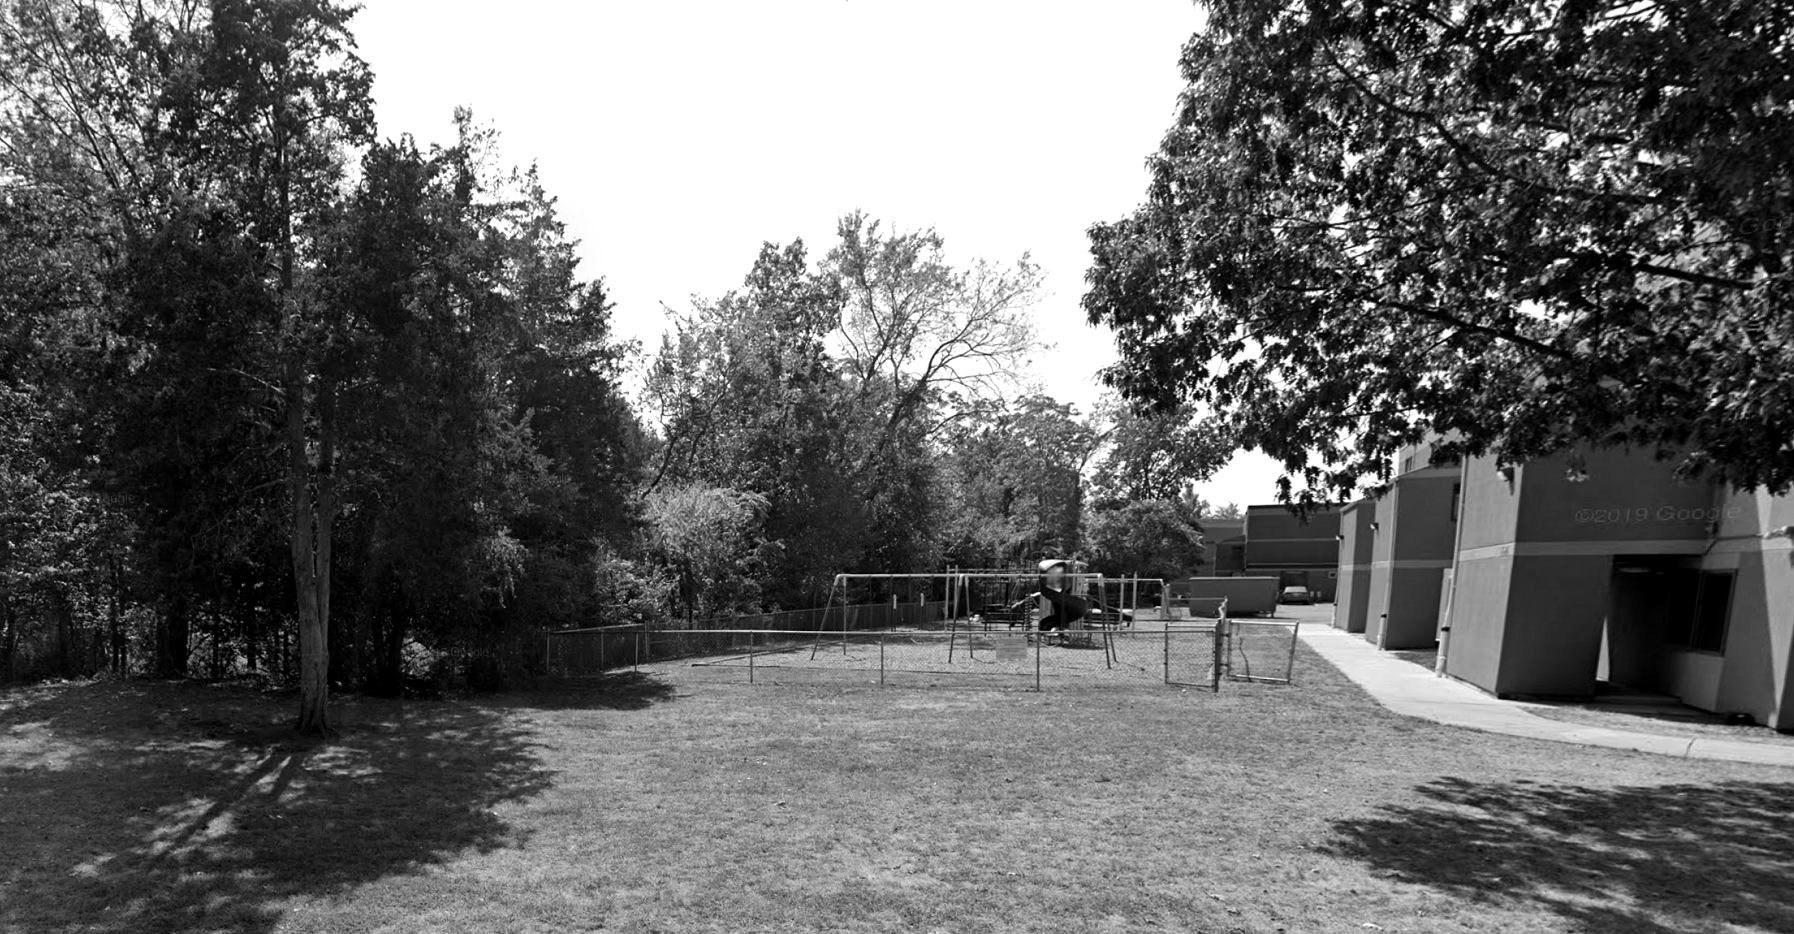
\includegraphics[height=150mm]{figures/cover_gray.png}};
  \end{scope}

  % ---- 中间：深红色的横带（页面顶端往下 164--182 mm），写英文副标题 ----
  \shade[left color=coverred!85!black, right color=coverred, opacity=0.94]
    ($(current page.north west) + (0,-164mm)$) rectangle ($(TR) + (0,-182mm)$);
  \node[anchor=east, text=white, font=\coverfont\fontsize{27}{32}\selectfont]
    at ($(TR) + (-24mm,-173mm)$) {\CoverEnSubtitle};

  % ---- 中文书名左边的空白处：一张小小的、彩色的猫狗大战，像一张贴上去的相片 ----
  % 原图 1204×772 像素，trim 裁掉底部 112 像素（水印和 START 按钮）
  \node[rotate=-5, fill=white, inner sep=1.8mm,
        drop shadow={opacity=0.4, shadow xshift=0.8mm, shadow yshift=-0.8mm}]
    at ($(current page.north west) + (52mm,-139mm)$)
    {
\includegraphics[trim=0 112 0 0, clip, width=56mm]{figures/catdog.png}};

  % ---- 右上角：竖着的红色小标签 ----
  \fill[coverred] ($(TR) + (-27mm,-18mm)$) rectangle ++(12mm,-36mm);
  \node[rotate=90, text=white, font=\coverfont\itshape\fontsize{11}{13}\selectfont]
    at ($(TR) + (-21mm,-36mm)$) {\CoverEdition};

  % ---- 上半部：作者名，下面是英文书名和中文书名，都靠右 ----
  \node[anchor=east, text=covergray, font=\coverfont\fontsize{16}{19}\selectfont]
    at ($(TR) + (-24mm,-86mm)$) {\CoverAuthor};
  \node[anchor=north east, text=black!78,
        font=\coverfont\fontsize{62}{62}\selectfont\addfontfeature{LetterSpace=3}]
    at ($(TR) + (-21mm,-94mm)$) {\CoverEnTitle};
  \node[anchor=north east, text=black!78, font=\CJKfamily{coverkai}\fontsize{44}{48}\selectfont]
    at ($(TR) + (-24mm,-124mm)$) {\CoverZhTitle};

  % ---- 左下角：“出版社”的标志 ----
  \fill[white, opacity=0.88] ($(current page.south west) + (14mm,14mm)$) rectangle ++(31mm,19mm);
  \node[text=coverred, font=\coverfont\bfseries\fontsize{30}{30}\selectfont]
    at ($(current page.south west) + (24mm,26mm)$) {C};
  \node[text=covergray, font=\coverfont\fontsize{19}{19}\selectfont]
    at ($(current page.south west) + (35.5mm,26.5mm)$) {\{\,\}};
  \node[text=covergray, font=\coverfont\fontsize{6.5}{8}\selectfont\addfontfeature{LetterSpace=10}]
    at ($(current page.south west) + (29.5mm,17.8mm)$) {LAZY PRESS};
\end{tikzpicture}

\end{titlepage}
\thispagestyle{empty}\null\clearpage
%! TeX root = ../main-zh.tex
% 献词页：放在封面之后、前言之前，单独一页，不印页眉页码
\cleardoublepage
\thispagestyle{empty}
\vspace*{0.28\textheight}
\begin{flushright}
  \itshape\large
  To my dog Ray and cat Summer.\\[0.8em]
  Seriously, this book is for you two.\\[0.8em]
  Now go study.
\end{flushright}
\clearpage

%! TeX root = ../../main-zh.tex
\chapter{前言}

真传一句话，假传万卷书。具体到计算机里的某一项技能，一句话当然说不完。但一个人想学计算机体系结构，也别上来就给他推荐《计算机体系结构：量化研究方法》（\emph{Computer Architecture: A Quantitative Approach}），这谁能看懂。

我想先讲讲自己是怎么走到 CPU 这里来的。

小时候，我很想知道计算机是怎么工作的，但从来不敢去想硬件是怎么造出来的。在我眼里，硬件像是凭空长出来的魔法，就像这个世界本来的设定一样摆在那里。不会去质疑它，甚至不会去好奇它是怎么工作的。只知道 CPU 一年比一年快，自己的电脑很快就落伍了。

到了高中和大学，我开始学黑客技术。对我来说，它是一条通往底层软件的通道，是我的“White rabbit”——就像《爱丽丝梦游仙境》里那只白兔，跟着它，就掉进了另一个世界。这一次，我终于敢去好奇了：那些黑客工具是怎么做出来的？

我先后学了 Pascal、BASIC，后来是 C。然后知道了“API”这个词，它是操作系统提供的服务；顺便也才弄明白，原来还有一个东西叫操作系统。等到我能调用 Win32 API 的时候，比起在 C 里用 \texttt{printf} 打印三角形，我觉得自己一下子有了力量，好像在计算机的世界里，没有什么是我做不到的。

然后是汇编，再接着是读泄露出来的 Windows 内核代码，也读开源的 Linux 内核代码。我试着写驱动，也想过写一个小小的操作系统。但这件事我其实没有做成，学过《Linux 内核完全注释》。这本书逐行注释了 Linux 0.11 内核的源代码。大学时，我还在一台真实的 PC 上装起了 Linux 0.11 内核。

我还自己写过一个 TCP 协议栈。当时我写的 rootkit 能绕过所有商业软件防火墙，但传数据很慢，因为我的做法是发一个包、确认一次，再发下一个。为了解决这个问题，我从 4.4BSD 的代码里学会了滑动窗口。

做过不少 rootkit 项目之后，我的目光转向了更底层的东西，比如 CPU 是怎么工作的。x86 汇编只给了我一点线索，离真正弄懂 CPU 还差得很远：它是怎么工作的，长什么样子，我连想象都想象不出来。

那时我参加了一个项目：用软件模拟x86 CPU，在里面运行恶意代码。我负责内存模拟的部分。不过这部分做的大多还是操作系统层面的事，比如分页、保护页（guard page）、写时复制（copy-on-write）。内存其实不需要真的去模拟,模拟器本身就运行在内存里，只是模拟一些机制。但这正是我需要的那条线索。古人说“阅藏知津”，读经要先知道渡口在哪里。这个项目，就是我通往大海的那个渡口。

又过了几年，我自己写了一个 x86 CPU 模拟器。它并不完整，但我从中弄明白了怎样解析二进制代码，一条指令是怎样由操作码、ModR/M 字节这些部分组成的。我的 CPU 之旅，就是从这里真正开始的。

我不想让这些话听起来像是我已经走到了终点，好像已经知道怎么造出一颗现代 CPU。我离那里还很远。但我确实在往那里走，而且这条路在我眼前越来越清楚。

这本书，就是我沿着这条路留下的记录。我还在追逐着我的小白兔。
           % 占位
\tableofcontents
\listoflistings

\mainmatter
%! TeX root = ../../main-en.tex
% 译自: chapters/zh/ch01.tex @ 12b16dd:chapters/ch01.tex
\chapter{It Starts with Hello, world}
\label{chap:hello}

Almost every book on C begins with the same program:
\codefile{code/ch01/hello.c}{The simplest C program}{lst:hello}

It is only seven lines long. Everybody has written it, and there seems to be nothing to say about it. But it is actually a door. Between the moment you press Enter to compile it and the moment that line of text appears on the screen, it passes through the preprocessor, the compiler, the assembler, the linker and the operating system, and only then does the CPU execute its instructions, one at a time. This book is about the very bottom of that road: how a CPU is built. Before we set off, let us walk the whole road once, from one end to the other.

The examples for this chapter are in the \texttt{code/ch01/} directory. Run \texttt{make} in a WSL or Linux terminal and you can reproduce every file in this chapter, step by step. The output shown in the book comes from Ubuntu on x86-64 with GCC 15.2. With a different compiler version the details will differ, but the overall picture stays the same.

C has several versions of its international standard. All the code in this book follows \emph{C99}, the version published in 1999, and compiles with any common C compiler.

\section{Reading It Line by Line}

\paragraph{\texttt{\#include <stdio.h>}}
Lines starting with \texttt{\#} are not C statements; they are commands for the \emph{preprocessor}.\lazynote{Preprocessor}{The program that processes the source code before the real compilation: it expands \texttt{\#include}, replaces macros and strips comments.} \texttt{\#include} means something very plain: copy the contents of the file \texttt{stdio.h} right here, word for word. The angle brackets say ``look in the system header directories''. If you write \texttt{\#include "stdio.h"} instead, the directory of the current source file is searched first.

\texttt{stdio.h} is short for ``standard input/output header''. We need it because we are about to call \texttt{printf}.

\paragraph{\texttt{int main(void)}}
\texttt{main} is where the program starts---at least as far as C is concerned. \texttt{int} says that it returns an integer, and \texttt{void} says that it takes no arguments. The program begins with the first statement of \texttt{main}. Later we will see that some other code actually runs before \texttt{main}.

\paragraph{\texttt{printf("Hello, world!\textbackslash n");}}
This calls the function \texttt{printf} to print a string on the screen. \texttt{\textbackslash n} is the newline character. Note that \texttt{printf} is not part of the C language itself; it is an ordinary function in the C standard library. The C language has no input or output statements at all.

\paragraph{\texttt{return 0;}}
\texttt{main} returns 0, telling whoever called it that the program ended normally.\lazyhint{\texttt{\$?} is the shell's record of ``the exit status of the last program''. 0 means success; any other number means something went wrong.} After running the program in a terminal, type \texttt{echo \$?} and you will see that 0.

\section{What Is in a Header File}
\label{sec:stdio-h}

\texttt{printf} is not implemented in \texttt{stdio.h}. Open the file and have a look: it is mostly a long list of \emph{declarations} like these:\lazynote{Declaration}{Tells the compiler what a function is called, what arguments it takes and what it gives back, but does not contain the function's code.}
\begin{minted}[linenos=false]{c}
extern int printf (const char *__restrict __format, ...);
extern int puts (const char *__s);
\end{minted}

A declaration only tells the compiler what a function looks like: its name, the arguments it takes and the type it returns. With the declaration, the compiler can check that a call to \texttt{printf} is written correctly and knows how to pass the arguments. Where the code of \texttt{printf} lives, the compiler does not care---that is the linker's job.

So header files and libraries are two different things:
\begin{itemize}
  \item a header file (such as \texttt{stdio.h}) is a text file full of declarations, used at compile time;
  \item a library (such as \texttt{libc.so.6} on Linux) is compiled machine code, used at link time and at run time.\lazynote{Library}{A bundle of functions, written and compiled in advance, for other programs to use. Section~\ref{sec:library} builds one of our own.}
\end{itemize}

So where is \texttt{stdio.h}? GCC searches the following directories, in order:
\begin{minted}[linenos=false]{text}
/usr/lib/gcc/x86_64-linux-gnu/15/include
/usr/local/include
/usr/include/x86_64-linux-gnu
/usr/include
\end{minted}
and finally finds it at \texttt{/usr/include/stdio.h}. You can print this list with \texttt{echo | gcc -E -Wp,-v -}.

\section{From Source Code to Executable}
\label{sec:toolchain}

Normally we type just one command:
\begin{minted}[linenos=false]{text}
gcc hello.c -o hello
\end{minted}
But \texttt{gcc} is only the ``manager''. Behind the scenes it calls four tools in turn, and each step produces an intermediate file (Figure~\ref{fig:toolchain}). With the right options, you can make \texttt{gcc} stop after any step and look at what that step produced.

\begin{figure}[htbp]
  \centering
  \begin{tikzpicture}[
      node distance=4mm and 9mm,
      file/.style={draw, minimum width=19mm, minimum height=7mm, font=\ttfamily\small},
      tool/.style={font=\small, align=center},
      arr/.style={-{Stealth}, thick},
    ]
    \node[file]                 (c) {hello.c};
    \node[file, right=of c]     (i) {hello.i};
    \node[file, right=of i]     (s) {hello.s};
    \node[file, right=of s]     (o) {hello.o};
    \node[file, below=12mm of o] (x) {hello};
    \node[file, left=of x, dashed] (lib) {libc etc.};

    \draw[arr] (c) -- node[tool, above=1mm] {preprocess\\\texttt{-E}} (i);
    \draw[arr] (i) -- node[tool, above=1mm] {compile\\\texttt{-S}} (s);
    \draw[arr] (s) -- node[tool, above=1mm] {assemble\\\texttt{-c}} (o);
    \draw[arr] (o) -- node[tool, right=1mm] {link} (x);
    \draw[arr, dashed] (lib) -- (x);
  \end{tikzpicture}
  \caption{The four steps of gcc}
  \label{fig:toolchain}
\end{figure}

Here are the four commands from this chapter's Makefile. Step by step, they do the same job:
\begin{minted}[linenos=false]{text}
gcc -E hello.c -o hello.i      # 1. preprocess
gcc -S hello.i -o hello.s      # 2. compile
gcc -c hello.s -o hello.o      # 3. assemble
gcc hello.o -o hello           # 4. link
\end{minted}

Table~\ref{tab:hello-files} lists the file produced by each step. An 84-byte source file grows to more than twenty thousand bytes after preprocessing---all of it brought in by \texttt{stdio.h} and the other headers it includes.

\begin{table}[htbp]
  \centering
  \caption{Files produced by each step}
  \label{tab:hello-files}
  \small
  \begin{tabular}{llrl}
    \toprule
    File & Contents & Size (bytes) & Produced by \\
    \midrule
    \texttt{hello.c} & C source code            & 84      & the programmer \\
    \texttt{hello.i} & preprocessed C code      & 21\,439 & preprocessor \texttt{cpp} \\
    \texttt{hello.s} & assembly code            & 661     & compiler \texttt{cc1} \\
    \texttt{hello.o} & object file (machine code) & 1\,496 & assembler \texttt{as} \\
    \texttt{hello}   & executable               & 15\,952 & linker \texttt{ld} \\
    \bottomrule
  \end{tabular}
\end{table}

\subsection{Step 1: Preprocessing}

The preprocessor handles every line that starts with \texttt{\#}: it expands the files named by \texttt{\#include}, replaces macros and strips comments. Its output is still C code, just without the \texttt{\#include}.

Open \texttt{hello.i} and you will find more than eight hundred lines. Almost all of the beginning is type definitions and function declarations copied from header files, including the declarations of \texttt{printf} and \texttt{puts}. More than twenty header files have been pulled in, because \texttt{stdio.h} itself includes other headers. The code we actually wrote has been pushed all the way to the end of the file:
\codefile{code/ch01/hello_tail.i}{The last few lines of hello.i}{lst:hello-i}

The first line, \texttt{\# 3 "hello.c"}, is a marker the preprocessor leaves for the compiler. It means ``the following code comes from line 3 of \texttt{hello.c}''. When the compiler reports an error, it uses these markers to find the original line numbers.

\subsection{Step 2: Compiling}

The compiler, \texttt{cc1}, translates C code into assembly code.\lazynote{Assembly code}{The ``text version'' of machine instructions. Each line roughly corresponds to one CPU instruction, such as \texttt{call} or \texttt{ret}.} This is the most complicated step of the whole process: lexical analysis, parsing, type checking, optimization and code generation all happen here. The main part of \texttt{hello.s} is shown in Listing~\ref{lst:hello-s} (to make it easier to read, the debugging directives starting with \texttt{.cfi} and a few extra lines at the end of the file have been removed).

\codefile[gas]{code/ch01/hello_main.s}{The main part of hello.s (x86-64)}{lst:hello-s}

Lines starting with a dot, such as \texttt{.section} and \texttt{.globl}, are directives for the assembler, not instructions. Lines 2--4 put the string into the read-only data section (\texttt{.rodata}) and name it \texttt{.LC0}; line 5 switches back to the code section (\texttt{.text}); line 6 declares \texttt{main} as a global symbol so that the linker can find it. The real instructions start at \texttt{main:} on line 8. Even if you do not know x86 assembly yet, you can follow it roughly:
\begin{itemize}
  \item \texttt{endbr64} is a security marker for the CPU, used to block certain attacks. You can ignore it for now.
  \item \texttt{pushq \%rbp} and \texttt{movq \%rsp, \%rbp} set up the stack frame of \texttt{main}; the \texttt{popq \%rbp} at the end tears it down.
  \item \texttt{leaq .LC0(\%rip), \%rax} gets the address of the string, which is then moved into the register \texttt{rdi}. On x86-64 Linux, the first argument of a function is passed in \texttt{rdi}.
  \item \texttt{call puts@PLT} calls the function.
  \item \texttt{movl \$0, \%eax} puts the return value 0 into \texttt{eax}---this is \texttt{return 0}.
  \item \texttt{ret} returns.
\end{itemize}

Wait a moment. Why does it call \texttt{puts} and not \texttt{printf}?

\subsection{A Small Optimization by the Compiler}

\texttt{printf} is a complicated function: it scans the format string character by character, and whenever it meets a conversion specification such as \texttt{\%d} or \texttt{\%s}, it performs the matching conversion. Our string, however, contains no conversion specifications and ends with \texttt{\textbackslash n}. GCC knows that in this case \texttt{printf("Hello, world!\textbackslash n")} does exactly the same thing as \texttt{puts("Hello, world!")}---\texttt{puts} adds a newline at the end by itself. So it quietly swaps in the simpler, faster \texttt{puts}. Notice that the string \texttt{.LC0} referenced in Listing~\ref{lst:hello-s} is \texttt{"Hello, world!"}: the trailing \texttt{\textbackslash n} is gone.

This tells us two things.\lazynote{Built-in function}{A standard library function that the compiler knows about and treats specially, such as \texttt{printf} or \texttt{memcpy}.} First, the compiler knows the standard library better than we might think: functions such as \texttt{printf}, \texttt{memcpy} and \texttt{strlen} have special ``built-in'' versions in GCC. The compiler knows what they mean and optimizes them. Second, even with optimization turned off, the code the compiler generates is not necessarily a word-for-word translation of the source.

If you add the option \texttt{-fno-builtin}, telling GCC not to treat these functions as built-ins, the generated code will dutifully call \texttt{printf}.

\subsection{Step 3: Assembling}

The assembler, \texttt{as}, translates the assembly code into machine code and produces the \emph{object file} \texttt{hello.o}.\lazynote{Object file}{A compiled ``half-finished product''. It contains machine code, but the references to outside functions are still blank, waiting for the linker to fill them in.} Machine code is what the CPU really executes: a sequence of bytes. \texttt{objdump -d -r hello.o} disassembles it for us (Listing~\ref{lst:hello-o}).

\codefile[text]{code/ch01/hello_main.objdump}{Machine code of main in hello.o}{lst:hello-o}

On each line, the left column is the offset of the instruction within \texttt{main}, the middle is its machine code, and the right is the corresponding assembly instruction. You can see that x86 instructions come in different lengths: \texttt{push \%rbp} is a single byte, \texttt{55}, while \texttt{lea} takes seven bytes. The CPU has to work out how long an instruction is before it knows where the next one begins---this is one of the reasons x86 CPUs are hard to build, and we will come back to it when we talk about instruction encoding.

Now look at the \texttt{call} instruction at offset \texttt{12}.\lazynote{Relocation}{A ``to-do list'' inside an object file: which position needs to be filled with the address of which symbol.} Its machine code is \texttt{e8 00 00 00 00}. \texttt{e8} means ``call'', and the next four bytes should be the relative address of the function being called---but they are all zero. The line below it, \texttt{R\_X86\_64\_PLT32 puts-0x4}, is a \emph{relocation} entry. It says: ``The address of \texttt{puts} goes here, but I do not know where it is yet.'' Likewise, the \texttt{lea} instruction at offset \texttt{8} leaves four bytes blank, waiting for the address of the string.

\texttt{hello.o} is a ``half-finished product'': its own code has been translated into machine code, but its references to the outside world are still blank. \texttt{nm hello.o} shows that \texttt{main} is marked \texttt{T} (defined in the code section) and \texttt{puts} is marked \texttt{U} (undefined).

\subsection{Step 4: Linking}

The linker, \texttt{ld}, puts the object files and libraries together, fills in all the blank addresses and produces the executable.

The code of \texttt{puts} is in the C standard library, \texttt{libc.so.6}. This is a \emph{shared library}:\lazynote{Shared library}{A library that is loaded only when the program runs; many programs share the same copy in memory. On Linux its name ends in \texttt{.so}; on Windows it is a \texttt{.dll}.} at link time, the linker does not copy the code of \texttt{puts} into \texttt{hello}. It only notes that ``this program needs \texttt{libc.so.6}''. When the program runs, the dynamic linker \texttt{ld-linux-x86-64.so.2} loads the library into memory and fills in the real addresses. The PLT in \texttt{call puts@PLT} (Procedure Linkage Table) is a relay station set up for exactly this purpose. \texttt{ldd hello} shows the libraries the program depends on:
\begin{minted}[linenos=false]{text}
linux-vdso.so.1
libc.so.6 => /usr/lib/x86_64-linux-gnu/libc.so.6
/lib64/ld-linux-x86-64.so.2
\end{minted}

At link time, \texttt{gcc} also quietly adds a few object files we never wrote: \texttt{Scrt1.o}, \texttt{crti.o}, \texttt{crtbeginS.o}, \texttt{crtendS.o} and \texttt{crtn.o}. Run \texttt{gcc} with the option \texttt{-v} and you will see them in the link command. \texttt{Scrt1.o} contains a function called \texttt{\_start}, and that is the program's real entry point.

\section{After the Program Starts}
\label{sec:runtime}

Type \texttt{./hello} in the terminal, press Enter, and \texttt{Hello, world!} appears on the screen. In between, this is what happens:
\begin{enumerate}
  \item The terminal program (the shell) asks the operating system to run \texttt{hello}. The operating system reads the file, creates a new process for it and maps its code and data into memory.
  \item Because the program needs a shared library, the operating system first hands control to the dynamic linker. The dynamic linker loads \texttt{libc.so.6} and fills in the addresses of \texttt{puts} and the other functions.
  \item The program starts executing at \texttt{\_start}.\lazynote{Entry point}{The location of the first instruction executed after a program is loaded. The real entry point of a C program is \texttt{\_start}, not \texttt{main}.} It does some preparation, such as sorting out the command-line arguments, and then calls \texttt{main} through the C standard library.
  \item \texttt{main} calls \texttt{puts}.\lazynote{System call}{The way a program asks the operating system kernel to do something for it, such as writing to the screen. Covered in detail in Section~\ref{sec:syscall}.} \texttt{puts} puts the string into the standard output buffer and eventually makes the \texttt{write} system call, asking the operating system to write those bytes to the terminal.
  \item \texttt{main} returns 0. The C standard library then calls \texttt{exit(0)}, which writes out whatever is left in the buffer, and then uses the \texttt{exit\_group} system call to tell the operating system: this process is finished, and its exit status is 0.
\end{enumerate}

Here we finally reach the bottom of the software: a program cannot write on the screen by itself; it can only ask the operating system for help. And the operating system is just another program---every one of its instructions must, in the end, be executed by the CPU.

\section{What the CPU Sees}

Peel away all these layers and the CPU sees just one thing: a sequence of bytes in memory. The \texttt{55}, \texttt{48 89 e5}, \texttt{c3}\ldots{} in Listing~\ref{lst:hello-o} are what the CPU really has to deal with.

The CPU's job is a loop that never stops:
\begin{enumerate}
  \item \lazynote{Program counter}{A register inside the CPU that holds the memory address of the next instruction to execute; PC for short.}Fetch: read the bytes of an instruction from memory, at the address given by the program counter (called \texttt{rip} on x86-64);
  \item Decode: work out which instruction these bytes are and which registers it uses;
  \item Execute: do the arithmetic, or access memory;
  \item Write back: write the result to a register or to memory, and point the program counter at the next instruction.
\end{enumerate}

The functions, variables and types of C no longer exist at this level. All that is left are registers, memory addresses and instructions, one after another. \texttt{main} is an address, \texttt{"Hello, world!"} is fourteen bytes in memory (the last one is 0), and \texttt{return 0} is setting the register \texttt{eax} to 0.

From the next part on, we will build a CPU that does exactly this with our own hands: it will fetch, decode and execute, and it will run programs we write in C. To keep it simple, we will not build a CPU with instructions of varying length like x86; instead we will choose a more regular instruction set.

\section{Don't Close the Book Just Yet}
\label{sec:dont-quit}

All right. By now you are probably dizzy: preprocessing, object files, relocations, the PLT, dynamic linking, system calls\ldots{} plus screen after screen of assembly code and machine code. Are you about to close this book and toss it aside?

{\Large\bfseries But---}

\begin{center}
  \begin{tikzpicture}[scale=1.1, line width=1.2pt]
    % The two cheeks: the outline of two circles of radius 1 centred at (-0.72,0) and (0.72,0),
    % which meet at (0,±0.694)
    \filldraw[fill=pink!70]
      (0,0.694) arc[start angle=43.95, end angle=316.05, radius=1]
                arc[start angle=223.95, end angle=496.05, radius=1];
    % The crack in the middle
    \draw (0,0.694) .. controls (0.07,0.3) .. (0.02,-0.25);
    % Highlights
    \draw[white, line width=2.2pt, line cap=round]
      (-1.3,0.42) arc[start angle=150, end angle=115, radius=0.7];
    \draw[white, line width=2.2pt, line cap=round]
      (0.22,0.58) arc[start angle=150, end angle=115, radius=0.7];
    % Blush
    \fill[red!40, opacity=0.5] (-0.95,-0.35) ellipse[x radius=0.22, y radius=0.12];
    \fill[red!40, opacity=0.5] ( 0.95,-0.35) ellipse[x radius=0.22, y radius=0.12];
    % Wiggle
    \foreach \s in {-1, 1} {
      \draw[gray, line width=0.8pt, line cap=round]
        (\s*1.95, 0.35) arc[start angle=90-\s*90+\s*30, end angle=90-\s*90-\s*30, radius=0.4];
      \draw[gray, line width=0.8pt, line cap=round]
        (\s*2.2, 0.5) arc[start angle=90-\s*90+\s*35, end angle=90-\s*90-\s*35, radius=0.65];
    }
  \end{tikzpicture}

  \smallskip
  (No, not that butt.)
\end{center}

Hear me out!

\begin{center}
  {\Large\bfseries You don't need to understand any of that yet.}
\end{center}

Really. These are the things the rest of this book will peel back, one layer at a time. This chapter just lets you stand at the door and glance at how deep it goes inside. If you didn't follow it, that is perfectly normal; if you followed all of it right now, there would be no need to write the rest of the book.

For now you only need to do one thing: treat Listing~\ref{lst:hello} as a template. Copy the \texttt{\#include <stdio.h>}, \texttt{int main(void)} and \texttt{\{} at the top, and the \texttt{return 0;} and \texttt{\}} at the bottom, exactly as they are---don't change a single character. In between, write one \texttt{printf} line for each thing you want to print, as many lines as you like:

\codefile{code/ch01/hey.c}{Print whatever you like}{lst:hey}

There are only three rules:
\begin{itemize}
  \item put what you want to print inside a pair of double quotes;
  \item \texttt{\textbackslash n} means ``new line''; add it wherever you want the line to break;
  \item don't forget the semicolon \texttt{;} at the end of every \texttt{printf(...)} line.
\end{itemize}

Save it as \texttt{hey.c}, then compile and run it:
\begin{minted}[linenos=false]{text}
gcc hey.c -o hey
./hey
\end{minted}
\needspace{14\baselineskip}
and this appears on the screen:
\inputminted[linenos=false]{text}{code/ch01/hey.out}

Make the triangle as big as you like. Use \texttt{*}, use \texttt{@}, or any other character. Want to show your dad what you made? Replace \texttt{Hey Dad!} with whatever you want to say to him. Typos are no big deal either: \texttt{gcc} will tell you which line is wrong; fix it and compile again.

\bigskip
\begin{center}
  {\Large\bfseries Congratulations---you are already writing C programs!}
\end{center}
\bigskip

\section{Summary}

\begin{itemize}
  \item \texttt{\#include <stdio.h>} copies in the contents of a header file. Header files contain only declarations; the code of the functions is in libraries.
  \item \texttt{gcc} calls the preprocessor, the compiler, the assembler and the linker in turn, producing the \texttt{.i}, \texttt{.s} and \texttt{.o} files and the executable.
  \item The compiler optimizes based on what it knows about the standard library, for example by replacing \texttt{printf} with \texttt{puts}.
  \item Calls to outside functions in an object file are still blank; the linker and the dynamic linker fill in the real addresses.
  \item The real entry point of a program is \texttt{\_start}, not \texttt{main}; output is finally done by the operating system through system calls.
  \item The CPU sees only instruction bytes in memory. It fetches, decodes, executes and writes back, over and over.
  \item You don't need to understand any of this yet. Use Hello, world as a template, write \texttt{printf} lines in the middle, and you are already writing C programs.
\end{itemize}

\section*{Exercises}

\begin{enumerate}
  \item Following Listing~\ref{lst:hey}, use \texttt{printf} to print a picture of your own design: a Christmas tree, an arrow, or the initials of your name.
  \item Run \texttt{make} in the \texttt{code/ch01/} directory, then open \texttt{hello.i} and find the declarations of \texttt{printf} and \texttt{puts}.
  \item Change the string in \texttt{hello.c} to \texttt{"Hello, \%s!\textbackslash n"} and add an argument \texttt{"world"}. Regenerate \texttt{hello.s}. Does it call \texttt{printf} or \texttt{puts} this time? Think about why.
  \item Delete the line \texttt{\#include <stdio.h>} and compile again. What error or warning does GCC give?
  \item Run \texttt{objdump -d} on both \texttt{hello.o} and \texttt{hello}, and compare the machine code of the \texttt{call} instruction in \texttt{main}. What is different?
\end{enumerate}

%! TeX root = ../../main-zh.tex
\chapter{C 语言的基本功}
\label{chap:c-basics}

上一章，我们把 Hello, world 当成模板，在中间写 \texttt{printf}，让计算机打印出想打印的东西。这一章，我们要让程序真正“动”起来：会记住数，会算数，会读入你敲的键盘，会做决定，还会不知疲倦地重复做同一件事。

学完这些，程序就能做很多事了。本章最后，我们会只用这些最基本的东西，写一个可以玩的文字冒险游戏。

本章的所有示例都在 \texttt{code/ch02/} 目录中。在 WSL 或 Linux 终端中进入这个目录，运行 \texttt{make} 编译全部程序，运行 \texttt{make test} 可以自动检查每个程序的输出。书中显示的运行结果，都是这些程序真正运行的结果。

\section{变量：贴了标签的盒子}
\label{sec:variable}

\codefile{code/ch02/var.c}{变量和加法}{lst:var}

运行结果：
\inputminted[linenos=false]{text}{code/ch02/out/var.txt}

\texttt{int a = 3;} 的意思是：准备一个能装整数的盒子，贴上标签 \texttt{a}，往里面放进 3。这个盒子就是\emph{变量}\lazynote{变量}{程序里一个有名字的存储位置，可以放进一个值，也可以随时换掉。}，标签就是变量的名字，盒子里装的东西是变量的\emph{值}（图~\ref{fig:boxes}）。\texttt{int} 是 integer（整数）的缩写，说明这个盒子只能装整数。

\begin{figure}[htbp]
  \centering
  \begin{tikzpicture}[line width=0.8pt]
    \foreach \x/\n/\v in {0/a/3, 2.9/b/4, 5.8/c/7} {
      \filldraw[fill=brown!30]  (\x,0) rectangle +(1.6,1.2);
      \filldraw[fill=brown!15]  (\x,1.2) -- +(0.4,0.3) -- +(2.0,0.3) -- +(1.6,0) -- cycle;
      \filldraw[fill=brown!45]  (\x+1.6,0) -- +(0.4,0.3) -- +(0.4,1.5) -- +(0,1.2) -- cycle;
      \node[font=\huge\bfseries] at (\x+0.8,0.6) {\v};
      \node[draw, fill=yellow!40, rotate=8, font=\ttfamily\large,
            inner sep=3pt] at (\x+0.8,-0.4) {\n};
    }
    \node[font=\huge] at (2.45,0.7) {+};
    \node[font=\huge] at (5.35,0.7) {=};
    \node[font=\small, align=left, anchor=west] at (8.0,1.0)
      {\texttt{c = a + b;}\\[2pt]把 a、b 盒子里的数相加，\\放进 c 盒子};
  \end{tikzpicture}
  \caption{变量就像一个个贴了标签的盒子}
  \label{fig:boxes}
\end{figure}

\texttt{int c;} 只准备了盒子，没有往里面放东西。这时 \texttt{c} 里装的是什么？谁也不知道，可能是任何一个数。所以在用一个变量之前，一定要先给它一个值。

\texttt{c = a + b;} 先取出 \texttt{a} 和 \texttt{b} 的值，算出 $3 + 4 = 7$，再把 7 放进 \texttt{c}。注意，C 语言里的 \texttt{=} 不是数学里的“等于”，而是“放进去”的意思，叫做\emph{赋值}\lazynote{赋值}{把 \texttt{=} 右边算出来的值放进左边的变量。和数学里的“等于”不是一回事。}。所以 \texttt{a = 10;} 把 \texttt{a} 里原来的 3 倒掉，换成 10。在数学里，下面这个式子是不成立的：
\begin{minted}[linenos=false]{c}
x = x + 1;
\end{minted}
在 C 语言里却再正常不过：取出 \texttt{x} 的值，加 1，再放回 \texttt{x}。效果就是让 \texttt{x} 增加 1。后面我们会经常这样写。

\texttt{printf} 也有了新本事。字符串里的 \texttt{\%d} 是一个“空位”，表示“这里填一个整数”。字符串后面跟着几个值，就依次填进这几个空位：第一个 \texttt{\%d} 填 \texttt{a}，第二个填 \texttt{b}，第三个填 \texttt{c}。

变量的名字可以用英文字母、数字和下划线，但不能以数字开头，也不能用 \texttt{int}、\texttt{if} 这些 C 语言已经占用的词。大小写是不同的：\texttt{a} 和 \texttt{A} 是两个变量。名字最好能说明盒子里装的是什么，比如 \texttt{score}、\texttt{count}。

C 语言里除了 \texttt{int}，还有能装小数的 \texttt{double}、能装字符的 \texttt{char} 等类型。本章只用 \texttt{int}，已经够我们做很多事了。

\section{算术运算：让程序做数学}
\label{sec:arith}

\codefile{code/ch02/arith.c}{加减乘除和取余}{lst:arith}

运行结果：
\inputminted[linenos=false]{text}{code/ch02/out/arith.txt}

C 语言的五种算术运算如表~\ref{tab:arith} 所示。

\begin{table}[htbp]
  \centering
  \caption{算术运算}
  \label{tab:arith}
  \begin{tabular}{cll}
    \toprule
    运算符 & 含义 & 例子 \\
    \midrule
    \texttt{+} & 加 & \texttt{17 + 5} 得 22 \\
    \texttt{-} & 减 & \texttt{17 - 5} 得 12 \\
    \texttt{*} & 乘 & \texttt{17 * 5} 得 85 \\
    \texttt{/} & 除（整数相除时，只要商） & \texttt{17 / 5} 得 3 \\
    \texttt{\%} & 取余数 & \texttt{17 \% 5} 得 2 \\
    \bottomrule
  \end{tabular}
\end{table}

有两点要特别注意：
\begin{itemize}
  \item 乘号是 \texttt{*}，不是 $\times$；
  \item 两个整数相除，结果还是整数\lazyhint{想要算出小数，要用 \texttt{double} 类型的变量，比如 \texttt{17.0 / 5} 得 3.4。}，小数部分直接扔掉：\texttt{17 / 5} 得 3，不是 3.4。想知道扔掉了多少，就用 \texttt{\%} 取余数：$17 = 5 \times 3 + 2$，所以 \texttt{17 \% 5} 得 2。
\end{itemize}

取余数看起来不起眼，其实很有用：一个数除以 2 余 0，它就是偶数；秒数除以 60 的余数，就是不满一分钟的那几秒。下一节我们就会用到它。

计算的顺序和数学一样：先乘除，后加减，有括号先算括号里的。因为 \texttt{\%} 在 \texttt{printf} 的字符串里有特殊含义，要打印一个 \texttt{\%}，得写成 \texttt{\%\%}。

最后，盒子的大小是有限的。\texttt{int} 能装的数大约在正负 21 亿之间（准确地说，最大是 2\,147\,483\,647）。一年有 31\,536\,000 秒，还装得下；一百年的秒数就装不下了，算出来会是一个莫名其妙的数。

\section{从键盘读入：\texorpdfstring{\NoCaseChange{scanf}}{scanf}}
\label{sec:scanf}

到现在为止，程序里的数都是写死的。要让程序和人互动，就要能读入键盘上敲的东西。\texttt{printf} 负责“说”，\texttt{scanf} 负责“听”：

\codefile{code/ch02/add.c}{读入两个数，算出它们的和}{lst:add}

运行一下，敲入 \texttt{3 4}，按回车：
\inputminted[linenos=false]{text}{code/ch02/out/add.txt}

\texttt{scanf("\%d \%d", \&a, \&b)} 的意思是：从键盘读入两个整数，第一个放进 \texttt{a}，第二个放进 \texttt{b}。和 \texttt{printf} 一样，\texttt{\%d} 表示一个整数。

变量名前面的 \texttt{\&} 千万不能忘\lazyhint{忘了写 \texttt{\&} 是新手最常见的错误之一。为什么要写它，第~\ref{sec:swap}~节揭晓。}。为什么要加它，等学到“指针”时再解释；现在只要记住：\textbf{用 \texttt{scanf} 读入变量时，变量名前面加 \texttt{\&}}。

如果敲的不是数字，比如敲了 \texttt{abc}，会怎么样？\texttt{scanf} 读不出整数，\texttt{a} 和 \texttt{b} 里就什么也没放进去。好在 \texttt{scanf} 会告诉我们它成功读入了几个数。代码中 \texttt{if (scanf(...) != 2)} 的意思是：“如果读到的不是两个数”，就打印一句提示，然后 \texttt{return 1;} 结束程序。返回 1 而不是 0，是告诉系统：程序没有正常完成。本章后面的程序，每次调用 \texttt{scanf} 都会这样检查一下。

\section{\texorpdfstring{\NoCaseChange{if}}{if} 和 \texorpdfstring{\NoCaseChange{else}}{else}：做决定}
\label{sec:if}

程序不能总是从头走到尾，有时候要根据情况做不同的事。比如，判断一个数是奇数还是偶数：

\codefile{code/ch02/even_odd.c}{奇数还是偶数}{lst:even-odd}

\inputminted[linenos=false]{text}{code/ch02/out/even_odd.txt}

\texttt{if} 后面的括号里是一个\emph{条件}\lazynote{条件}{结果是“成立”或“不成立”的式子。在 C 语言里，0 表示不成立，非 0 表示成立。}。\texttt{n \% 2 == 0} 问的是：“\texttt{n} 除以 2 的余数等于 0 吗？”如果是，就执行紧跟着的那对花括号里的代码；否则，执行 \texttt{else} 后面那对花括号里的代码。两条路，只走一条（图~\ref{fig:fork}）。

\begin{figure}[htbp]
  \centering
  \begin{tikzpicture}[line width=0.8pt]
    \draw[gray, line width=1pt] (-3.8,0) -- (3.6,0);
    \fill[brown!60!black] (0,0) rectangle (0.2,3.3);
    \filldraw[fill=green!25]
      (0,2.4) -- (-3.2,2.4) -- (-3.6,2.7) -- (-3.2,3.0) -- (0,3.0) -- cycle;
    \node at (-1.75,2.7) {\texttt{if}（条件成立）};
    \filldraw[fill=orange!30]
      (0.2,1.6) -- (2.9,1.6) -- (3.3,1.9) -- (2.9,2.2) -- (0.2,2.2) -- cycle;
    \node at (1.6,1.9) {\texttt{else}（否则）};
    % 站在路口挠头的小人
    \draw (-1.8,1.25) circle (0.18);
    \draw (-1.8,1.07) -- (-1.8,0.5);
    \draw (-1.8,0.5) -- (-2.0,0) (-1.8,0.5) -- (-1.6,0);
    \draw (-1.8,0.9) -- (-2.1,0.65);
    \draw (-1.8,0.9) -- (-1.55,1.15) -- (-1.62,1.38);
    \node[red!70!black, font=\Large\bfseries] at (-2.15,1.7) {?};
  \end{tikzpicture}
  \caption{走哪条路，由条件决定}
  \label{fig:fork}
\end{figure}

如果不止两种情况，可以用 \texttt{else if} 一个接一个地问下去：

\codefile{code/ch02/grade.c}{按分数给评价}{lst:grade}

\inputminted[linenos=false]{text}{code/ch02/out/grade.txt}

程序从上往下依次检查每个条件，遇到第一个成立的，就执行它的代码，后面的都不再看了。所以 95 分只会得到“优秀”，不会同时得到“良好”和“及格”。前面的条件都不成立时，才执行最后的 \texttt{else}。

花括号里的代码往右缩进了四个空格。缩进对程序的运行没有影响，但能让人一眼看出哪些代码属于哪个 \texttt{if}。养成好习惯，从现在开始。

\section{比较和逻辑运算}
\label{sec:logic}

\texttt{if} 的条件，通常是用表~\ref{tab:compare-ops} 中的运算符写出来的。

\begin{table}[htbp]
  \centering
  \caption{比较运算和逻辑运算}
  \label{tab:compare-ops}
  \begin{tabular}{cll}
    \toprule
    运算符 & 含义 & 例子 \\
    \midrule
    \texttt{==} & 等于     & \texttt{n == 5} \\
    \texttt{!=} & 不等于   & \texttt{n != 5} \\
    \texttt{<}  & 小于     & \texttt{n < 5} \\
    \texttt{>}  & 大于     & \texttt{n > 5} \\
    \texttt{<=} & 小于或等于 & \texttt{n <= 5} \\
    \texttt{>=} & 大于或等于 & \texttt{n >= 5} \\
    \midrule
    \texttt{\&\&} & 并且：两个条件都成立 & \texttt{n > 0 \&\& n < 10} \\
    \texttt{||}   & 或者：至少一个成立   & \texttt{n < 0 || n > 10} \\
    \texttt{!}    & 不：把成立变成不成立 & \texttt{!(n > 0)} \\
    \bottomrule
  \end{tabular}
\end{table}

用 \texttt{\&\&} 和 \texttt{||} 可以把几个条件组合起来。判断闰年就是一个好例子：能被 4 整除但不能被 100 整除，或者能被 400 整除的年份，是闰年。

\codefile{code/ch02/leap.c}{判断闰年}{lst:leap}

\inputminted[linenos=false]{text}{code/ch02/out/leap.txt}

在 C 语言看来，“成立”和“不成立”其实就是数：条件成立时结果是 1，不成立时是 0。反过来，\texttt{if} 和后面要讲的 \texttt{while} 只看括号里的值是不是 0：是 0 就当作不成立，不是 0 就当作成立。所以 \texttt{if (playing)} 的意思就是“如果 \texttt{playing} 不是 0”。本章最后的游戏里会用到这种写法。

\begin{quote}
  \textbf{当心 \texttt{=} 和 \texttt{==}！}判断相等要用两个等号。如果把 \texttt{if (n == 5)} 写成 \texttt{if (n = 5)}，意思就变成了“把 5 放进 \texttt{n}，然后看 \texttt{n} 是不是 0”——条件永远成立，\texttt{n} 原来的值也被改掉了。这是 C 语言里最常见的错误之一，而且 \texttt{gcc} 默认一声不吭。编译时加上 \texttt{-Wall} 选项（意思是 warn all，打开所有常用的警告），\texttt{gcc} 就会提醒你：
\begin{minted}[linenos=false]{text}
warning: suggest parentheses around assignment used as truth value
\end{minted}
  建议以后编译时都加上 \texttt{-Wall}：\texttt{gcc -Wall hello.c -o hello}。
\end{quote}

\section{\texorpdfstring{\NoCaseChange{while}}{while} 循环：重复做一件事}
\label{sec:while}

计算机最擅长的，就是不知疲倦地重复。\texttt{while} 的意思是“当……的时候”：只要条件成立，就一遍又一遍地执行花括号里的代码。

\codefile{code/ch02/countdown.c}{火箭倒计时}{lst:countdown}

\inputminted[linenos=false, lastline=3]{text}{code/ch02/out/countdown.txt}
\vspace{-0.5\baselineskip}
\begin{center}（中间省略）\end{center}
\vspace{-0.5\baselineskip}
\inputminted[linenos=false, firstline=10]{text}{code/ch02/out/countdown.txt}

\begin{center}
  \begin{tikzpicture}[line width=0.8pt]
    \filldraw[fill=orange!70, draw=orange!80!red] (0.12,0) -- (0.4,-1.0) -- (0.68,0) -- cycle;
    \filldraw[fill=yellow!80, draw=yellow!80!orange] (0.26,0) -- (0.4,-0.55) -- (0.54,0) -- cycle;
    \filldraw[fill=red!60] (0,0.05) -- (-0.4,-0.35) -- (0,0.7) -- cycle;
    \filldraw[fill=red!60] (0.8,0.05) -- (1.2,-0.35) -- (0.8,0.7) -- cycle;
    \filldraw[fill=gray!10] (0,0) rectangle (0.8,2.2);
    \filldraw[fill=red!60] (0,2.2) -- (0.4,3.0) -- (0.8,2.2) -- cycle;
    \filldraw[fill=cyan!30] (0.4,1.55) circle (0.2);
    \node[font=\Huge\bfseries]  at (2.3,2.5) {3};
    \node[font=\LARGE\bfseries] at (3.3,1.9) {2};
    \node[font=\Large\bfseries] at (4.1,1.3) {1};
    \node[font=\Large\bfseries, red!70!black] at (5.4,0.6) {发射！};
    \foreach \y in {-1.3,-1.6} \draw[gray, line width=0.6pt] (-0.1,\y) -- (0.9,\y);
  \end{tikzpicture}
\end{center}

程序是这样执行的：
\begin{enumerate}
  \item 检查条件 \texttt{n > 0}。一开始 \texttt{n} 是 10，条件成立。
  \item 执行花括号里的代码：打印 \texttt{10...}，然后 \texttt{n = n - 1}，\texttt{n} 变成 9。
  \item 回到第 1 步，再检查一次条件……
\end{enumerate}
就这样，\texttt{n} 从 10 一路减到 1。当 \texttt{n} 变成 0 时，条件不成立了，循环结束，程序接着执行循环后面的 \texttt{printf("发射！\textbackslash n")}。

注意循环里的 \texttt{n = n - 1;} 这一行。如果忘了写它，\texttt{n} 永远是 10，条件永远成立，程序就会没完没了地打印 \texttt{10...}——这叫\emph{死循环}\lazynote{死循环}{条件永远成立、永远停不下来的循环。在终端里按 \texttt{Ctrl+C} 可以让程序停下。}。万一写出了死循环，别慌，在终端里按 \texttt{Ctrl+C} 就能让程序停下来。

\texttt{while} 最适合事先不知道要重复多少次的情况。比如猜数字，谁也不知道要猜几次才能猜中：

\codefile{code/ch02/guess.c}{猜数字}{lst:guess}

\inputminted[linenos=false]{text}{code/ch02/out/guess.txt}

只要 \texttt{guess != secret}，也就是还没猜中，就一直让玩家猜下去。每猜一次，\texttt{tries} 就加 1，最后告诉玩家一共猜了几次。

每次都从中间猜，最多 7 次就一定能猜中 1 到 100 之间的任何一个数。你能想明白为什么吗？

\section{\texorpdfstring{\NoCaseChange{for}}{for} 循环：数着数重复}
\label{sec:for}

据说德国数学家高斯上小学时，老师为了让学生们安静一会儿，出了一道题：从 1 加到 100 等于几？别的孩子还在一个一个地加，小高斯很快就举手了：$1 + 100 = 101$，$2 + 99 = 101$……一共 50 对，所以答案是 $50 \times 101 = 5050$。

\begin{center}
  \begin{tikzpicture}[line width=0.8pt]
    \filldraw[fill=green!30!black, draw=brown!60!black, line width=3pt] (0,0) rectangle (6.4,1.9);
    \node[white] at (3.2,0.95) {$1 + 2 + 3 + \cdots + 100 = \;?$};
    % 举手的小高斯
    \draw (7.4,1.05) circle (0.2);
    \draw (7.4,0.85) -- (7.4,0.3);
    \draw (7.4,0.3) -- (7.2,-0.2) (7.4,0.3) -- (7.6,-0.2);
    \draw (7.4,0.7) -- (7.15,0.45);
    \draw (7.4,0.7) -- (7.7,1.55);
    \node[draw, rounded corners, fill=yellow!20, font=\bfseries] (say) at (8.7,2.1) {5050！};
    \draw (say.south west) ++(0.3,0) -- (7.65,1.3);
    \draw[gray, line width=1pt] (-0.2,-0.2) -- (9.6,-0.2);
  \end{tikzpicture}
\end{center}

我们没有高斯那么聪明，但是我们有计算机，可以老老实实地一个一个加：

\codefile{code/ch02/sum.c}{从 0 加到 100}{lst:sum}

\inputminted[linenos=false]{text}{code/ch02/out/sum.txt}

和高斯算的一样！对计算机来说，加一百次也就是一眨眼的事。

\texttt{for} 后面的括号里有三部分，用分号隔开：
\begin{minted}[linenos=false]{c}
for (i = 0; i <= 100; i++) {
\end{minted}
\begin{enumerate}
  \item \texttt{i = 0}：开始之前先做一次，给计数的变量一个初值；
  \item \texttt{i <= 100}：每一圈开始之前检查的条件，成立才继续；
  \item \texttt{i++}：每一圈结束之后做的事。\texttt{i++} 是 \texttt{i = i + 1} 的简写。
\end{enumerate}
所以 \texttt{i} 依次是 0、1、2……100，每一圈都把 \texttt{i} 加进 \texttt{sum}。其实 \texttt{for} 循环能做的事，\texttt{while} 循环都能做；但像这样“从几数到几”的时候，用 \texttt{for} 把三部分写在一行里，看得更清楚。

循环里还可以再套循环。还记得第~\ref{chap:hello}~章里一行一行手写的三角形吗？现在可以想要多大就打印多大了：

\codefile{code/ch02/triangle.c}{打印任意大小的三角形}{lst:triangle}

\inputminted[linenos=false]{text}{code/ch02/out/triangle.txt}

外面的 \texttt{for} 一行一行地往下走，\texttt{row} 是行号。对于第 \texttt{row} 行，里面的两个 \texttt{for} 先打印 \texttt{n - row} 个空格，再打印 \texttt{2 * row - 1} 个星号，最后换行。第 1 行是 1 个星号，第 2 行是 3 个，第 3 行是 5 个……一个三角形就出来了。

\section{\texorpdfstring{\NoCaseChange{break}}{break}：提前离开循环}
\label{sec:break}

有时候，循环还没走完，我们已经找到了想要的东西，就可以用 \texttt{break} 提前离开：

\codefile{code/ch02/first_square.c}{第一个平方大于 2000 的数}{lst:first-square}

\inputminted[linenos=false]{text}{code/ch02/out/first_square.txt}

\texttt{i} 从 1 开始往上数。数到 45 时，$45 \times 45 = 2025$，比 2000 大了，\texttt{break} 立即跳出循环，后面的 46、47……都不再检查。这时 \texttt{i} 里留下的就是 45。

\texttt{break} 只跳出它所在的那一层循环。第~\ref{chap:c-structure}~章还会讲到 \texttt{break} 的一种巧妙用法。

\section{小游戏：龙洞寻宝}
\label{sec:dragon}

学到这里，我们已经会用变量记住东西，会读入玩家的选择，会用 \texttt{if} 做决定，会用循环重复。这些就够写一个游戏了！

\begin{center}
  \begin{tikzpicture}[line width=0.9pt]
    % 龙尾巴，绕在宝箱前面
    \draw[red!70!black, line width=5pt, line cap=round]
      (-1.6,1.0) .. controls (-1.4,-0.6) and (1.0,-0.55) .. (2.5,-0.25);
    \filldraw[fill=red!70!black, draw=red!70!black]
      (2.45,-0.05) -- (2.95,-0.25) -- (2.45,-0.45) -- (2.6,-0.25) -- cycle;
    % 宝箱
    \filldraw[fill=brown!55, draw=brown!40!black] (0,0) rectangle (2.4,1.2);
    \filldraw[fill=brown!45, draw=brown!40!black]
      (0,1.2) -- (0,1.45) arc[start angle=180, end angle=0, x radius=1.2, y radius=0.45]
      -- (2.4,1.2) -- cycle;
    \fill[yellow!70!orange] (0.35,0) rectangle (0.55,1.2) (1.85,0) rectangle (2.05,1.2);
    \filldraw[fill=yellow!70!orange, draw=brown!40!black] (1.03,0.85) rectangle (1.37,1.3);
    \fill[black] (1.2,1.03) circle (0.05);
    % 金币
    \foreach \x/\y in {3.1/0.1, 3.5/0.1, 3.9/0.1, 3.3/0.32, 3.7/0.32, 3.5/0.54} {
      \filldraw[fill=yellow!80!orange, draw=orange!80!black]
        (\x,\y) ellipse[x radius=0.2, y radius=0.09];
    }
    % 呼噜声
    \node[font=\Large\bfseries, rotate=12]  at (-1.2,2.0) {Z};
    \node[font=\large\bfseries, rotate=12]  at (-0.75,2.45) {z};
    \node[font=\normalsize\bfseries, rotate=12] at (-0.4,2.8) {z};
  \end{tikzpicture}

  \smallskip
  （嘘——龙在打呼噜）
\end{center}

\subsection{游戏规则}

传说山里的龙洞中藏着一箱金币。你举着火把，站在了洞口。洞里有四个地方（图~\ref{fig:cave-map}）：洞口、岔路口、一个小房间，还有龙穴。宝箱就在龙穴里，一条大红龙正趴在上面睡觉。

\begin{figure}[htbp]
  \centering
  \begin{tikzpicture}[
      place/.style={draw, rounded corners, fill=brown!10, minimum width=22mm,
                    minimum height=12mm, align=center},
      way/.style={thick, {Stealth}-{Stealth}},
    ]
    \node[place]                     (door)  {洞口\\\texttt{\small room = 1}};
    \node[place, right=18mm of door] (fork)  {岔路口\\\texttt{\small room = 2}};
    \node[place, above right=4mm and 18mm of fork] (small) {小房间\\\texttt{\small room = 3}};
    \node[place, below right=4mm and 18mm of fork, fill=red!10] (lair) {龙穴\\\texttt{\small room = 4}};
    \draw[way] (door) -- (fork);
    \draw[way] (fork) -- node[above left, font=\small] {左} (small);
    \draw[way] (fork) -- node[below left, font=\small] {右} (lair);
    \node[right=2mm of small, font=\small, align=left] {墙上挂着\\一把钥匙};
    \node[right=2mm of lair, font=\small, align=left] {龙和宝箱};
  \end{tikzpicture}
  \caption{龙洞地图}
  \label{fig:cave-map}
\end{figure}

每一步，游戏会告诉你在哪里、可以做什么，你输入选项的编号。要小心：火把只够烧 12 步，烧完了就什么也看不见了。至于怎样才能拿到宝箱……自己去试试吧。小提示：龙好像喜欢数学好的人。

\needspace{12\baselineskip}
\subsection{程序}

\codefile{code/ch02/dragon.c}{龙洞寻宝}{lst:dragon}

\subsection{玩一局}

\inputminted[linenos=false]{text}{code/ch02/out/dragon.txt}

（剧透：这只是其中一种玩法。小房间里的钥匙有什么用？你自己去发现吧。）

\subsection{游戏是怎样做出来的}

这个程序有一百多行，看起来很长，其实用到的全是本章讲过的东西。

\paragraph{用变量记住游戏的状态。}程序开头的几个变量，记录了游戏此刻的全部情况：\texttt{room} 记住你在哪里，用 1、2、3、4 代表四个地方；\texttt{has\_key} 记住你有没有钥匙，0 表示没有，1 表示有；\texttt{torch} 记住火把还能烧几步；\texttt{playing} 记住游戏是否还在进行。游戏世界里发生的一切，归根到底就是这几个盒子里的数在变化。

\paragraph{用一个大循环让游戏一直进行下去。}\texttt{while (playing)} 是整个游戏的主循环。只要 \texttt{playing} 不是 0，就一圈一圈地转下去。每一圈都做三件事：
\begin{enumerate}
  \item \textbf{描述}：根据 \texttt{room} 的值，用 \texttt{if}/\texttt{else if} 打印出这个地方的样子和可以做的事；
  \item \textbf{读入}：用 \texttt{scanf} 读入玩家的选择，同时火把少烧一步；
  \item \textbf{更新}：根据“在哪里”和“选了什么”，改变变量的值——走到别的地方就改 \texttt{room}，拿到钥匙就把 \texttt{has\_key} 设为 1，游戏结束就把 \texttt{playing} 设为 0。
\end{enumerate}
玩家看到的“走进山洞”“拿起钥匙”，在程序里不过是 \texttt{room = 2;} 和 \texttt{has\_key = 1;} 而已。

\paragraph{龙的谜题。}龙问的正是 \texttt{for} 循环那一节算过的题。这里用一个 \texttt{for} 循环给玩家 3 次机会，答对了就用 \texttt{break} 提前离开循环，同时把 \texttt{won} 设为 1。循环结束后，如果 \texttt{won} 还是 0，说明 3 次都没答对。

这种“描述—读入—更新”的循环，叫做\emph{游戏循环}\lazynote{游戏循环}{描述、读入、更新，一圈一圈地转下去。几乎所有的游戏都是这个结构。}。从最简单的文字游戏，到画面精美的大型游戏，用的都是这个结构，只不过大型游戏每秒要转几十圈。还记得第~\ref{chap:hello}~章最后讲到的 CPU 吗？它也在转着一个永不停歇的循环：取指、译码、执行、写回。看来，循环真是计算机世界的心跳。

\subsection{动手改一改}

游戏是你的了，随便改：
\begin{itemize}
  \item 把火把改成只能烧 8 步，看看还能不能拿到宝箱；
  \item 换一道谜题，比如“1 加到 1000 等于几”，或者让龙问你的生日；
  \item 增加一个地方，比如小房间后面的地下河。给它一个新的 \texttt{room} 编号，在“描述”和“更新”两部分各加一段 \texttt{else if}；
  \item 增加一个新的物品，比如一把剑。用一个新的变量 \texttt{has\_sword} 记住有没有拿到它。
\end{itemize}
改完了，运行 \texttt{make test} 看看原来的玩法还对不对。如果你改了游戏的规则，测试报告“失败”是正常的，那说明它在认真检查。

\section{小结}

\begin{itemize}
  \item 变量是贴了标签的盒子。\texttt{int} 型的变量装整数；\texttt{=} 是赋值，把右边的值放进左边的变量。
  \item 算术运算有 \texttt{+ - * / \%}。整数相除只要商，\texttt{\%} 取余数。
  \item \texttt{printf} 用 \texttt{\%d} 打印整数，\texttt{scanf} 用 \texttt{\%d} 读入整数，变量名前要加 \texttt{\&}。
  \item \texttt{if}/\texttt{else if}/\texttt{else} 根据条件选择要执行的代码。判断相等用 \texttt{==}，不是 \texttt{=}；编译时加上 \texttt{-Wall}。
  \item \texttt{\&\&}、\texttt{||}、\texttt{!} 组合条件。C 语言中 0 表示不成立，非 0 表示成立。
  \item \texttt{while} 在条件成立时重复执行；\texttt{for} 适合“从几数到几”；\texttt{break} 提前离开循环。死循环用 \texttt{Ctrl+C} 停止。
  \item 一个游戏，就是用变量记住状态，在一个循环中不断地描述、读入、更新。
\end{itemize}

\section*{练习}

\begin{enumerate}
  \item 写一个程序，读入一个秒数，比如 3725，打印出它是几小时几分几秒（1 小时 2 分 5 秒）。提示：用 \texttt{/} 和 \texttt{\%}。
  \item 修改代码~\ref{lst:sum}，算出 1 到 100 中所有偶数的和。（答案是 2550。）
  \item 用 \texttt{for} 循环打印九九乘法表。
  \item 修改代码~\ref{lst:guess}，如果猜了 7 次还没猜中，就告诉玩家答案并结束游戏。
  \item 修改代码~\ref{lst:triangle}，打印一个倒过来的三角形。
  \item 给龙洞寻宝增加一个新的地方和一件新的物品，再写一段测试，加进 \texttt{test.sh}。
\end{enumerate}
                 % 占位
%! TeX root = ../../main-zh.tex
\chapter{C 程序的结构}
\label{chap:c-structure}

设计 CPU 的过程中，C 语言几乎无处不在：启动代码之后的初始化程序、外设驱动、操作系统内核、验证用的测试程序，都是用 C 写的。本章不讲 C 的语法，而是讨论一个更实际的问题：一个函数应该组织成什么样子。

C 语言没有异常，也没有析构函数。一个函数往往要依次执行好几个可能失败的操作——打开文件、分配内存、申请硬件资源——每一步都要检查返回值；一旦失败，还要把前面已经拿到的资源一一释放。这部分代码常常比完成功能的代码还多。如果没有固定的写法，函数很快就会变得难以阅读，资源泄漏、重复释放这类错误也会随之出现。

经过多年的实践，大型 C 代码库形成了几种固定的写法。Windows 内核代码常把函数主体包在一个只执行一次的 \texttt{do \{ \} while (FALSE)} 循环里，出错时用 \texttt{break} 跳出；Linux 内核则用 \texttt{goto} 跳到函数末尾的清理代码。写法不同，思想相同：
\begin{itemize}
  \item \textbf{成功路径自上而下}\lazynote{成功路径}{每一步都顺利时，程序走过的那条路。好的函数让它从上到下一条直线走到底。}：如果每一步都成功，代码从函数顶部一直执行到底部，中间没有层层嵌套。读者从上往下读一遍，就知道这个函数做了什么。
  \item \textbf{失败路径统一出口}：任何一步失败，都立即离开主流程，到函数末尾的同一段清理代码，由它释放资源并返回错误码。
\end{itemize}

本章先用一个具体的例子说明没有这种结构时会出现什么问题，然后依次介绍只执行一次的循环、\texttt{goto} 和提前返回三种写法，最后总结配套的编程习惯。

本章的示例代码都在 \texttt{code/ch03/} 目录中。除 Windows 驱动的例子外，其余代码都可以在 Linux 上用 \texttt{make test} 编译和测试。

\section{一个例子：把文件读入内存}
\label{sec:load-file}

本章的各种写法都实现同一个函数：把一个文件的全部内容读入一块新分配的内存。
\begin{minted}[linenos=false]{c}
int load_file(const char *path, char **out, size_t *out_len);
\end{minted}
约定如下：
\begin{itemize}
  \item 成功时返回 0，\texttt{*out} 指向以 \texttt{'\textbackslash 0'} 结尾的缓冲区，\texttt{*out\_len} 是文件长度。缓冲区由调用者用 \texttt{free} 释放。
  \item 失败时返回负的错误码，例如文件不存在时返回 \texttt{-ENOENT}，这是 Linux 内核的习惯。此时 \texttt{*out} 为 \texttt{NULL}。
\end{itemize}

完成这个任务需要五步，每一步都可能失败，涉及两个资源：文件和缓冲区（表~\ref{tab:load-steps}）。越往后出错，需要释放的资源越多，这正是错误处理难写的原因。

\begin{table}[htbp]
  \begin{lazywide}
  \caption{读入文件的五个步骤}
  \label{tab:load-steps}
  \begin{tabular}{clll}
    \toprule
    步骤 & 操作 & 函数 & 失败时需要释放 \\
    \midrule
    1 & 打开文件     & \texttt{fopen}  & 无 \\
    2 & 移到文件末尾 & \texttt{fseek}  & 文件 \\
    3 & 取得文件长度 & \texttt{ftell}  & 文件 \\
    4 & 分配缓冲区   & \texttt{malloc} & 文件 \\
    5 & 读取内容     & \texttt{fread}  & 缓冲区、文件 \\
    \bottomrule
  \end{tabular}
  \end{lazywide}
\end{table}

\section{两种常见的坏写法}

\subsection{层层嵌套}

最直接的写法是“成功了才往下做”：每一步成功，就在 \texttt{if} 里面做下一步（代码~\ref{lst:nested}）。

\codefile{code/ch03/nested.c}{层层嵌套的写法}{lst:nested}

这段代码是正确的，但有三个问题：
\begin{enumerate}
  \item 成功路径——也就是这个函数真正要做的事——被推到了第六层缩进。步骤越多，代码越往右偏，整体形状像一个箭头，所以这种代码有时被称为“箭头代码”（arrow code）\lazynote{箭头代码}{层层嵌套的 \texttt{if}，缩进越来越深，整段代码的形状像一个箭头。}。
  \item 每个 \texttt{else} 都离对应的 \texttt{if} 很远。看到 \texttt{err = -errno;} 时，要往上数括号，才能知道它处理的是哪一步的失败。
  \item 增加一个步骤，就要再加一层嵌套，并把后面的代码整体右移。
\end{enumerate}

\subsection{每个出错点各自清理}

另一种写法是出错就立即返回，在返回之前把已经拿到的资源释放掉（代码~\ref{lst:dup}）。

\codefile{code/ch03/dup_cleanup.c}{每个出错点各自清理的写法}{lst:dup}

嵌套没有了，成功路径也回到了左边，但清理代码被复制了多次：\texttt{fclose(fp)} 出现了五次。以后如果再增加一个资源，比如一把锁，就要找出所有的 \texttt{return}，逐一补上释放代码，漏掉一处就是一个资源泄漏\lazynote{资源泄漏}{拿到的资源（内存、文件、锁……）用完了却没有还回去。}。

重复的代码里还容易藏着细节错误。注意 \texttt{fseek} 失败的分支：必须先把 \texttt{errno} 保存到 \texttt{err}，再调用 \texttt{fclose}，因为 \texttt{fclose} 可能改写 \texttt{errno}。\lazynote{\texttt{errno}}{C 标准库记录“上一次出错原因”的变量，会被后来的库函数调用改写。}如果写成 \texttt{fclose(fp); return -errno;}，返回的就可能是错误的错误码。这种细节要在每一个出错点都写对，很难保证。

\section{原则：成功路径自上而下}
\label{sec:happy-path}

好的结构如图~\ref{fig:happy-path} 所示：成功路径是左边一条直线，从上走到下；每一步失败时都向右离开，汇合到底部同一段清理代码。成功路径最后也经过这段清理代码。

\begin{figure}[htbp]
  \centering
  \begin{tikzpicture}[
      node distance=5mm,
      box/.style={draw, rounded corners, minimum width=34mm, minimum height=7mm},
      ok/.style={-{Stealth}, thick},
      fail/.style={red!70!black, dashed},
    ]
    \node[box]               (s1) {1. 打开文件};
    \node[box, below=of s1]  (s2) {2. 移到文件末尾};
    \node[box, below=of s2]  (s3) {3. 取得文件长度};
    \node[box, below=of s3]  (s4) {4. 分配缓冲区};
    \node[box, below=of s4]  (s5) {5. 读取内容};
    \node[box, below=of s5]  (s6) {交出缓冲区};
    \node[box, below=8mm of s6, fill=gray!10] (c) {清理资源，返回状态};

    \foreach \a/\b in {s1/s2, s2/s3, s3/s4, s4/s5, s5/s6, s6/c}
      \draw[ok] (\a) -- (\b);

    \coordinate (rail) at ($(s1.east) + (16mm, 0)$);
    \foreach \s in {s1, s2, s3, s4, s5}
      \draw[fail] (\s.east) -- (\s.east -| rail);
    \draw[fail, -{Stealth}] (s1.east -| rail) -- (c.east -| rail) -- (c.east);

    \node[right=1mm of rail |- s3, red!70!black, align=left]
      {失败\\（\texttt{break} 或 \texttt{goto}）};
    \node[left=6mm of s3, align=center] {成功路径\\自上而下};
  \end{tikzpicture}
  \caption{成功路径与统一出口}
  \label{fig:happy-path}
\end{figure}

具体来说，有四条规则：
\begin{enumerate}
  \item \textbf{开头初始化。}函数开头把所有资源变量设为“空”值（指针为 \texttt{NULL}，文件描述符为 $-1$），把状态变量设为一个表示失败的值。这样，清理代码只要看变量是否为空，就知道这个资源有没有拿到。
  \item \textbf{调用、检查、离开。}每一步都写成“调用 → 检查返回值 → 失败就离开”。成功时不缩进，直接往下走。
  \item \textbf{统一出口。}所有失败都到函数末尾的同一段清理代码。资源按与获取相反的顺序释放。
  \item \textbf{一个 \texttt{return}。}函数只在末尾返回一次，返回的就是状态变量。
\end{enumerate}

“离开”有两种方式：在只执行一次的循环里 \texttt{break}，或者 \texttt{goto} 到函数末尾的标签。下面两节分别介绍。

\section{模式一：只执行一次的循环}
\label{sec:do-while}

\subsection{原理}

\begin{minted}[linenos=false]{c}
do {
    /* 函数主体：任何一步失败就 break */
} while (FALSE);
/* 清理代码 */
\end{minted}

条件 \texttt{FALSE} 为假，所以循环体只执行一次，和一个普通的代码块没有区别。但它毕竟是循环，可以在里面使用 \texttt{break}：\texttt{break} 会立即跳到循环后面的第一条语句。于是，\texttt{do \{ \} while (FALSE)} 就成了一个“可以随时跳出的代码块”：主体放在循环里，清理代码放在循环后面，任何一步失败就 \texttt{break}。

\texttt{FALSE} 是 Windows 头文件中定义的宏，值为 0。在其他环境中，同样的写法是 \texttt{do \{ \} while (0)}。

\begin{quote}
  \textbf{注意：}一定要写成 \texttt{do \{ \} while (FALSE);}。如果写成 \texttt{while (FALSE) \{ \}}，条件在进入循环之前就判断为假，循环体一次也不会执行。
\end{quote}

\subsection{Windows 内核中的例子}

代码~\ref{lst:nt} 在 Windows 内核驱动中实现同样的功能。驱动程序中通常调用 \texttt{ZwCreateFile} 等 \texttt{Zw} 系列函数，它们与用户态的 \texttt{NtCreateFile} 等函数参数相同。这段代码需要 Windows 驱动开发包（WDK）\lazynote{WDK}{Windows Driver Kit，微软提供的编写 Windows 驱动程序的工具和头文件。}才能编译。

\codefile{code/ch03/nt_read.c}{Windows 内核中的 do-while(FALSE) 写法}{lst:nt}

这段代码有几个要点：
\begin{itemize}
  \item \texttt{status} 一开始设为 \texttt{STATUS\_UNSUCCESSFUL}，\texttt{file} 和 \texttt{data} 初始化为 \texttt{NULL}。
  \item 每次调用系统函数后，用 \texttt{NT\_SUCCESS(status)} 检查\lazynote{\texttt{NTSTATUS}}{Windows 内核函数返回的状态码。\texttt{NT\_SUCCESS} 判断它是不是表示成功。}。失败就 \texttt{break}，这时 \texttt{status} 里已经是系统函数返回的错误码。
  \item 不是系统函数返回的错误，例如文件为空、文件太大、内存分配失败，要在 \texttt{break} 之前自己给 \texttt{status} 赋值。这一点最容易忘记：如果漏写，\texttt{status} 里还是上一步成功时的 \texttt{STATUS\_SUCCESS}，函数就会在什么也没做成的情况下报告成功。
  \item 全部成功后，把 \texttt{data} 交给调用者，并把 \texttt{data} 置为 \texttt{NULL}，后面的清理代码就不会释放它。“交出所有权后置空”这个技巧，让成功和失败可以共用同一段清理代码。
  \item 循环结束后先检查 \texttt{status}，失败时输出调试信息；然后按与获取相反的顺序释放资源，最后返回 \texttt{status}。
\end{itemize}

\subsection{需要注意的地方}

\begin{itemize}
  \item \texttt{break} 只跳出最内层的循环或 \texttt{switch}。如果主体里还有 \texttt{for} 循环或 \texttt{switch}，其中的 \texttt{break} 不会跳到清理代码。这时要先设置状态，跳出内层之后再 \texttt{break} 一次。
  \item 不要在 \texttt{do \{ \} while (FALSE)} 里使用 \texttt{continue}。\texttt{continue} 会跳到循环条件处，条件为假，于是循环结束。效果和 \texttt{break} 一样，但读者很难看出这一点。
  \item 不要嵌套多层 \texttt{do \{ \} while (FALSE)}，否则很难看出每个 \texttt{break} 跳到哪里。
  \item 有的编译器在较高的警告级别下，会对 \texttt{while (FALSE)} 给出“条件表达式是常量”的警告。
\end{itemize}

在 Windows 上，微软的结构化异常处理（SEH）也能写出同样的结构：主体放在 \texttt{\_\_try} 块中，用 \texttt{\_\_leave} 跳出，清理代码放在 \texttt{\_\_finally} 块中。思路与 \texttt{do \{ \} while (FALSE)} 相同。

\section{模式二：\texorpdfstring{\NoCaseChange{goto}}{goto} 统一出口}
\label{sec:goto}

1968 年，Dijkstra 发表了著名的短文《Go To Statement Considered Harmful》\cite{dijkstra1968}，此后 \texttt{goto} 在很多教材里成了禁忌。Dijkstra 反对的是用 \texttt{goto} 在程序中随意跳转，使控制流难以追踪。只向前跳到函数末尾清理代码的 \texttt{goto} 不会造成这个问题，反而比前面几种写法更清楚。Linux 内核的编码规范专门有一节，推荐用 \texttt{goto} 集中处理函数的退出\cite{linux-coding-style}。

\subsection{单一出口标签}

代码~\ref{lst:goto-single} 只有一个标签 \texttt{out}，所有失败都跳到这里。

\codefile{code/ch03/goto_single.c}{goto 到单一出口}{lst:goto-single}

它的结构和 \texttt{do \{ \} while (FALSE)} 几乎一样：\texttt{break} 换成了 \texttt{goto out}，循环后面的代码换成了标签 \texttt{out:} 后面的代码。区别在于：
\begin{itemize}
  \item 没有伪装成循环的代码块，读者不需要先想明白“这个循环只执行一次”。
  \item \texttt{goto} 可以从任意深度的循环或 \texttt{switch} 中直接跳到出口，不存在 \texttt{break} 只能跳出一层的问题。
\end{itemize}

清理代码中，\texttt{free(buf)} 不需要判断 \texttt{buf} 是否为空，因为 C 标准规定 \texttt{free(NULL)} 什么也不做；\texttt{fclose} 没有这个保证，所以要先判断 \texttt{fp}。

这种写法要求所有资源变量在第一个 \texttt{goto} 之前就已经初始化为空值，否则清理代码会去释放一个还没拿到的资源。Linux 内核的编码规范把这类错误称为“one err bug”\cite{linux-coding-style}。

\subsection{分层标签}

Linux 内核中更常见的是代码~\ref{lst:ladder} 这样的写法：每个资源对应一个标签，标签按与获取资源相反的顺序排列。

\codefile{code/ch03/goto_ladder.c}{分层标签（Linux 内核风格）}{lst:ladder}

读法是：哪一步失败，就跳到释放“在它之前已经拿到的资源”的那个标签。例如 \texttt{fread} 失败时，缓冲区和文件都已经拿到，所以跳到 \texttt{err\_free}；执行完 \texttt{free(buf)} 后，代码继续往下执行到 \texttt{err\_close}，关闭文件。\texttt{malloc} 失败时还没有缓冲区，所以直接跳到 \texttt{err\_close}。

这种写法的优点是清理代码不需要判断变量是否为空，每个标签只做一件事；增加资源时，只需在释放它的位置加一个标签。缺点是成功路径要在标签之前自己释放不再需要的资源（这里是 \texttt{fclose}）并返回，所以函数有两个 \texttt{return}；如果跳错了标签，就会泄漏或重复释放资源。

Linux 内核的编码规范建议标签名说明它做什么，比如 \texttt{err\_free}，而不是 \texttt{err1}、\texttt{err2}\cite{linux-coding-style}。这样增删步骤时不用给标签重新编号，检查每个 \texttt{goto} 是否跳对了也更容易。

\subsection{使用 goto 的规则}

\begin{itemize}
  \item 只向前跳，而且只跳到函数末尾的清理代码。
  \item 不要跳进 \texttt{if} 或循环等代码块的内部。
  \item 不要跳过变量的初始化。C 语言不允许从可变长数组（VLA）的作用域之外跳进它的作用域；C++ 不允许跳过带初始化的变量声明。把变量都声明在函数开头，可以避免这个问题。
  \item 标签名说明它做什么。
\end{itemize}

\section{模式三：提前返回}
\label{sec:early-return}

如果函数出错时还没有拿到任何资源，就不需要统一出口，直接 \texttt{return} 最清楚。最常见的是函数开头的参数检查，例如设置串口波特率的函数：
\begin{minted}[linenos=false]{c}
int uart_set_baud(struct uart *u, unsigned int baud)
{
    if (u == NULL)
        return -EINVAL;
    if (baud == 0 || baud > UART_MAX_BAUD)
        return -ERANGE;

    u->regs->div = u->clk_hz / (16 * baud);
    return 0;
}
\end{minted}

这种写法称为“卫语句”（guard clause）\lazynote{卫语句}{函数开头的几道“门卫”：条件不满足就立即返回，剩下的代码只管成功路径。}：先把不满足条件的情况排除掉，剩下的代码就是成功路径。代码~\ref{lst:ladder} 中，第一步 \texttt{fopen} 失败时也直接返回，因为这时还没有任何资源需要释放。

提前返回和统一出口可以一起使用：先用几个提前返回检查参数，再进入用 \texttt{goto} 或 \texttt{do \{ \} while (FALSE)} 组织的主体。规则只有一条：一旦拿到了需要释放的资源，就不要再直接 \texttt{return}。

\section{三种写法的比较}

表~\ref{tab:compare} 对比了本章介绍的几种写法。

\begin{table}[htbp]
  \begin{lazywide}
  \small
  \caption{几种错误处理写法的比较}
  \label{tab:compare}
  \begin{tabular}{L{2.4cm}L{1.8cm}L{3.0cm}L{3.0cm}L{3.0cm}}
    \toprule
    写法 & 离开方式 & 清理代码 & 适用场合 & 主要风险 \\
    \midrule
    \texttt{do \{ \} while (FALSE)} & \texttt{break} & 循环之后，判断资源是否为空 & Windows 代码；规范不允许 \texttt{goto} 的项目 & 内层循环或 \texttt{switch} 中的 \texttt{break} 跳不出去 \\
    \addlinespace
    \texttt{goto} 单一标签 & \texttt{goto out} & 标签之后，判断资源是否为空 & 一般的 C 代码 & 资源变量没有初始化为空值 \\
    \addlinespace
    \texttt{goto} 分层标签 & \texttt{goto err\_xxx} & 每个标签释放一个资源 & Linux 内核风格；资源较多时 & 跳错标签 \\
    \addlinespace
    提前返回 & \texttt{return} & 无 & 还没有拿到任何资源时 & 拿到资源后仍然直接返回 \\
    \bottomrule
  \end{tabular}
  \end{lazywide}
\end{table}

选择哪一种，首先要看项目已有的规范。在一个已有的代码库里，与周围代码保持一致，比选择哪一种“更好”的写法重要得多。如果是新项目，\texttt{goto} 单一标签通常是最简单的选择。

\section{配套的编程习惯}

\begin{itemize}
  \item \textbf{释放函数接受空值。}\texttt{free(NULL)} 什么也不做，所以清理代码可以直接写 \texttt{free(buf)}。自己写的释放函数也应该接受 \texttt{NULL}，调用方就不用每次判断。
  \item \textbf{交出所有权后置空。}把资源交给调用者或其他模块之后，立即把本地变量置为空值，清理代码就不会释放它（代码~\ref{lst:nt} 和代码~\ref{lst:goto-single}）。
  \item \textbf{及时保存错误码。}\texttt{errno} 会被后面的库函数调用改写，Windows 的 \texttt{GetLastError()} 也一样。出错后要立即把它保存到自己的变量里。
  \item \textbf{输出参数先置空。}函数开头把输出参数设为空值，调用者在失败时就不会拿到一个无效的指针。
  \item \textbf{不要用宏隐藏跳转。}\texttt{\#define CHECK(x) if (!(x)) goto out} 看起来能省几行，但读代码时看不到跳转，和 \texttt{if}/\texttt{else} 搭配时也容易出错。Linux 内核的编码规范也明确反对影响控制流的宏\cite{linux-coding-style}。
\end{itemize}

\section{编译器和其他语言的支持}

GCC 和 Clang 提供了 \texttt{\_\_attribute\_\_((cleanup(func)))}：变量离开作用域时，编译器自动调用 \texttt{func} 释放它。Linux 内核从 6.5 版本开始在 \texttt{include/linux/cleanup.h} 中基于这个特性提供了 \texttt{\_\_free()} 等辅助宏，一部分代码已经不再需要手写 \texttt{goto}。C++ 的析构函数（RAII）\lazynote{RAII}{C++ 的做法：资源跟着变量走，变量离开作用域时自动释放资源。}和 Rust 的 \texttt{Drop} 则把“离开作用域时释放资源”做进了语言本身。

不过，在启动代码、固件和大多数驱动程序中，我们写的仍然是标准 C。本章介绍的几种写法，仍然是写好这些代码的基本功。

\section{小结}

\begin{itemize}
  \item C 语言没有异常，每一步操作都要检查返回值，失败时要释放已经拿到的资源。
  \item 好的函数结构是：成功路径自上而下，失败路径统一出口。
  \item 实现统一出口有两种常用写法：Windows 风格的 \texttt{do \{ \} while (FALSE)} 加 \texttt{break}，以及 Linux 风格的 \texttt{goto}。还没有拿到资源时，可以直接提前返回。
  \item 配套的习惯包括：资源变量初始化为空值、交出所有权后置空、及时保存错误码、不用宏隐藏跳转。
\end{itemize}

\section*{练习}

\begin{enumerate}
  \item 把代码~\ref{lst:nested} 改写成 \texttt{do \{ \} while (0)} 的写法，保存为 \texttt{code/ch03/do\_while.c}，把它加入 \texttt{Makefile} 中的 \texttt{VARIANTS}，然后运行 \texttt{make test} 验证。
  \item 在代码~\ref{lst:ladder} 中增加第三个资源：读取成功后，再分配一块同样大小的缓冲区，把文件内容转换为大写后存入其中，并把这块缓冲区交给调用者。需要增加哪个标签？原来的哪些 \texttt{goto} 需要修改？
\end{enumerate}
                 % 占位
%! TeX root = ../../main-zh.tex
\chapter{内存与指针}
\label{chap:memory}

第~\ref{chap:c-basics}~章讲 \texttt{scanf} 时留了一个悬念：读入变量时，变量名前面为什么要加一个 \texttt{\&}？要回答这个问题，就得先弄清楚：程序里的变量，到底放在哪里？

这一章的前半部分讲内存：程序在内存里是什么样子，数据放在哪里，什么是栈，什么是堆，为什么用户程序碰不得操作系统内核。这些是计算机体系结构的基本概念，初学 C 的人不一定马上用得上；但心里有了这幅图，以后学指针、学操作系统、学 CPU，都会容易得多。后半部分讲指针——一个装着地址的变量。有了前面这幅图，指针就一点也不神秘了。

本章的示例在 \texttt{code/ch04/} 目录中。运行 \texttt{make} 编译，\texttt{make test} 检查。为了让地址短一些、好读一些，大部分程序都编译成了 \emph{32 位}的程序。至于 32 位、64 位是什么意思，第~\ref{sec:bits}~节会讲。

编译 32 位的程序，只要给 \texttt{gcc} 加上 \texttt{-m32}（需要先安装 \texttt{gcc-multilib}）：
\begin{minted}[linenos=false]{text}
gcc -m32 addr.c -o addr
./addr
\end{minted}
我们的电脑上运行的其实是 64 位的 Linux。为了让书中的地址和在真正的 32 位 Linux 上一模一样，而且每次运行都相同，本章的 Makefile 和脚本在编译、运行时还多加了几个选项（写在 \texttt{code/ch04/Makefile} 的注释里，不用管它们）。所以你自己运行时，看到的地址多半和书上不同，这很正常。

\section{内存：一排有门牌号的房子}
\label{sec:mem-street}

内存可以想象成一条很长很长的街，街边是一排一模一样的小房子。每座房子里只能住一个\emph{字节}\lazynote{字节}{8 个二进制位，能表示 0 到 255。内存是按字节编门牌号的。}（byte），也就是 8 个二进制位，能表示 0 到 255 之间的一个数。每座房子都有一个门牌号，这就是\emph{地址}。CPU 要读写内存，就得说出门牌号：“把 0xbffffdf4 号房子里的东西拿给我。”

在 C 语言里，变量名前面加上 \texttt{\&}，就能得到这个变量的地址：

\codefile{code/ch04/addr.c}{变量住在哪里}{lst:addr}

\inputminted[linenos=false]{text}{code/ch04/out/addr.txt}

几点说明：
\begin{itemize}
  \item \texttt{\&a} 读作“a 的地址”。\texttt{printf} 用 \texttt{\%p} 打印地址。前面的 \texttt{(void *)} 是告诉 \texttt{printf}“这是一个地址”，照抄即可。
  \item \texttt{sizeof(int)} 算出一个 \texttt{int} 占几个字节，要用 \texttt{\%zu} 打印。在我们的电脑上，一个 \texttt{int} 占 4 个字节，也就是要住 4 座房子。
  \item 地址是用\emph{十六进制}\lazynote{十六进制}{逢十六进一，用 \texttt{0}--\texttt{9} 和 \texttt{a}--\texttt{f}。两个十六进制数字正好是一个字节。}写的，前面的 \texttt{0x} 就是十六进制的标志。十六进制逢十六进一，用 \texttt{0}--\texttt{9} 和 \texttt{a}--\texttt{f} 这 16 个符号，\texttt{a} 是 10，\texttt{f} 是 15，\texttt{0x10} 是 16。地址很大，用十进制写太长，用十六进制正好：两个十六进制数字恰好是一个字节。
\end{itemize}

\texttt{a} 住在 \texttt{0xbffffdf4}，\texttt{b} 住在 \texttt{0xbffffdf8}，正好相差 4：\texttt{a} 占了 \texttt{0xbffffdf4} 到 \texttt{0xbffffdf7} 这 4 座房子，\texttt{b} 紧挨着住在后面（图~\ref{fig:houses}）。

\begin{figure}[htbp]
  \begin{lazywide}
  \begin{tikzpicture}[line width=0.7pt]
    \foreach \i/\v/\n in {0/03/f4, 1/00/f5, 2/00/f6, 3/00/f7, 4/04/f8, 5/00/f9, 6/00/fa, 7/00/fb} {
      \pgfmathsetmacro\x{\i*1.45}
      \filldraw[fill=yellow!15] (\x,0) rectangle +(1.15,0.9);
      \filldraw[fill=red!45] (\x-0.1,0.9) -- +(0.675,0.5) -- +(1.35,0) -- cycle;
      \filldraw[fill=brown!40] (\x+0.43,0) rectangle +(0.3,0.35);
      \node[font=\ttfamily\small] at (\x+0.575,0.63) {\v};
      \node[font=\ttfamily\tiny] at (\x+0.575,-0.22) {0xbffffd\n};
    }
    % 烟囱和炊烟
    \filldraw[fill=gray!40] (0.8,1.15) rectangle (0.97,1.55);
    \foreach \r/\dx/\dy in {0.08/0.05/0.12, 0.11/0.2/0.32, 0.14/0.42/0.58}
      \draw[gray!70] (0.88+\dx,1.55+\dy) circle (\r);
    \draw[decorate, decoration={brace, mirror, amplitude=6pt}]
      (0,-0.45) -- (5.5,-0.45) node[midway, below=7pt] {\texttt{int a = 3}，占 4 个字节};
    \draw[decorate, decoration={brace, mirror, amplitude=6pt}]
      (5.8,-0.45) -- (11.3,-0.45) node[midway, below=7pt] {\texttt{int b = 4}，占 4 个字节};
    \node[font=\small, anchor=west] at (11.5,0.6) {← 字节};
    \node[font=\small, anchor=west] at (11.5,-0.22) {← 地址};
  \end{tikzpicture}
  \caption{内存是一排有门牌号的房子，每座房子住一个字节}
  \label{fig:houses}
  \end{lazywide}
\end{figure}

仔细看图，3 这个数是怎样放进 4 个字节里的？它存成了 \texttt{03 00 00 00}：数值最低的那个字节，放在地址最小的房子里。这种存法叫\emph{小端}\lazynote{小端}{数值最低的字节放在地址最小的地方。反过来叫大端（big-endian）。}（little-endian）。x86 和 RISC-V 的处理器都是这样存数的。

\section{地址有多长：16 位、32 位和 64 位}
\label{sec:bits}

门牌号能写多长，决定了这条街最多能有多少座房子。地址如果有 $n$ 个二进制位，就能编出 $2^n$ 个不同的门牌号，也就是能访问 $2^n$ 个字节的内存。人们常说的“32 位”“64 位”，在这里指的就是地址有多少位。

同一个程序，可以编译成 32 位的，也可以编译成 64 位的：

\codefile{code/ch04/bits.c}{一个地址有多大}{lst:bits}

\inputminted[linenos=false]{text}{code/ch04/out/bits.txt}

32 位程序里的地址占 4 个字节，写成十六进制是 8 位数；64 位程序里的地址占 8 个字节，打印出来长了一大截。本章用 32 位的地址做例子，就是因为它短，好读；至于道理，32 位和 64 位是完全一样的。

\begin{figure}[htbp]
  \begin{lazywide}
  \begin{tikzpicture}[line width=0.8pt]
    \foreach \x/\plate/\label in {0/FFFF/16 位, 4.0/FFFFFFFF/32 位, 9.2/FFFFFFFFFFFFFFFF/64 位} {
      \filldraw[fill=yellow!15] (\x,0) rectangle +(2.0,1.5);
      \filldraw[fill=red!45] (\x-0.2,1.5) -- +(1.2,0.8) -- +(2.4,0) -- cycle;
      \filldraw[fill=brown!40] (\x+0.75,0) rectangle +(0.5,0.7);
      \node[draw, fill=blue!10, font=\ttfamily\small, inner sep=2pt] at (\x+1.0,1.12) {\plate};
      \node at (\x+1.0,-0.4) {\label};
    }
    % 64 位的门牌太长，挂不下，房子急得冒汗
    \fill[cyan!60] (11.55,2.05) ellipse (0.06 and 0.11);
    \fill[cyan!60] (11.75,1.8) ellipse (0.05 and 0.09);
    \draw[gray, line width=1pt] (-0.6,0) -- (12.0,0);
  \end{tikzpicture}
  \caption{门牌号越来越长}
  \label{fig:plates-grow}
  \end{lazywide}
\end{figure}

为什么地址会从 16 位变成 32 位，又变成 64 位？简单地说：内存越来越大，门牌号不够用了（表~\ref{tab:bits}）。

\begin{table}[htbp]
  \begin{lazywide}
  \small
  \caption{地址的位数和能访问的内存}
  \label{tab:bits}
  \begin{tabular}{L{3.8cm}L{2.4cm}L{5.4cm}L{1.8cm}}
    \toprule
    地址位数 & 能访问的内存 & 代表性的处理器 & 年代 \\
    \midrule
    16 位 & 64\,KB & Intel 8080、MOS 6502（Apple II、红白机） & 1970 年代 \\
    20 位（靠分段凑出来） & 1\,MB & Intel 8086（IBM PC） & 1978 年 \\
    32 位 & 4\,GB & Intel 80386 & 1985 年 \\
    64 位（目前实际用 48 位） & 256\,TB & AMD64（AMD Opteron） & 2003 年 \\
    \bottomrule
  \end{tabular}
  \end{lazywide}
\end{table}

\paragraph{16 位：64 KB 的小街。}
早期的微处理器，比如 Intel 8080 和 MOS 6502（苹果公司的 Apple II 电脑、任天堂的红白机都用它），地址是 16 位的，$2^{16} = 65\,536$，最多只能访问 64\,KB 内存。这在 1970 年代已经很奢侈了，可是程序越写越大，很快就不够用了。

1978 年，Intel 推出了 8086。它内部还是 16 位的，却想办法用 20 位的地址访问 1\,MB 内存：把内存分成一段一段的，地址由“段”和“段内的偏移”两部分组成，真正的地址是“段\,${}\times 16 +{}$\,偏移”。这就是\emph{分段}\lazynote{分段}{8086 的办法：地址 = 段 $\times$ 16 + 偏移，用两个 16 位的数凑出 20 位的地址。}。分段能用，但很别扭：一个地址要用两个数来表示，同一个地方可以有好多种写法，程序员写 C 语言时还得区分“近指针”和“远指针”。IBM PC 用的就是 8086 家族的处理器，1\,MB 中还有一部分要留给显示器和 BIOS，留给程序的只有 640\,KB。“640\,KB 内存”是那个年代许多程序员共同的记忆。

\paragraph{32 位：4 GB 的平坦大道。}
1985 年，Intel 推出 80386，地址变成了 32 位，$2^{32}$ 字节就是 4\,GB。更重要的是，从此可以不再分段：从 \texttt{0x00000000} 到 \texttt{0xffffffff}，所有的地址排成一条笔直的长街，这叫\emph{平坦}（flat）的地址空间。80386 还在硬件上支持了\emph{分页}\lazynote{分页}{把内存切成一页一页（通常 4\,KB），每一页可以单独映射、单独设置权限。}，让操作系统能给每个程序一个独立的、完整的 4\,GB 虚拟地址空间（第~\ref{sec:layout}~节最后会讲到）。1991 年，一个叫 Linus Torvalds 的芬兰大学生，就是在自己的 80386 电脑上开始写 Linux 的。前言里提到的 Linux 0.11，也是为 80386 写的。

\paragraph{64 位：4 GB 也不够了。}
4\,GB 在当时看来大得用不完，可是不到二十年，普通的电脑也装上了 4\,GB 内存。而且，一个 32 位程序能用的地址还到不了 4\,GB：32 位的 Linux 把其中 1\,GB 留给了操作系统内核（第~\ref{sec:kernel-space}~节），32 位的 Windows 默认只给程序 2\,GB。数据库、视频编辑、大型游戏，都被这道天花板压得喘不过气来。2003 年，AMD 推出了 64 位的 x86 处理器 AMD64，Intel 随后也跟进了。今天的电脑和手机，几乎都是 64 位的。

$2^{64}$ 字节是 16\,EB（约 172 亿 GB），远远超出了现在任何一台电脑的需要。所以今天的 x86-64 处理器实际上只用 48 位地址，可以访问 256\,TB；比较新的处理器可以用到 57 位。上面的 \texttt{bits64} 打印出的地址 \texttt{0x7fffffffecdc} 是 12 位十六进制数，正好是 48 位。

\paragraph{32 位并没有过时。}
64 位的处理器也能运行 32 位的程序，所以我们才能用 \texttt{gcc -m32} 编译出 32 位的程序，在 64 位的 Linux 上运行。上面 \texttt{bits32} 打印出的 \texttt{0xbffffdf4}，就是一个典型的 32 位 Linux 程序里的栈地址。洗衣机、路由器、手环里的小芯片，至今大多还是 32 位的；RISC-V 也有 32 位（RV32）和 64 位（RV64）两种。地址短一些，芯片就简单一些。对于从头开始造一颗 CPU 来说，32 位正是一个好的起点。

\section{程序住在内存的哪里}
\label{sec:layout}

一个程序运行起来，它的代码、全局变量、局部变量都要在内存里找地方住。它们住在哪里？写个程序看看：

\codefile{code/ch04/layout.c}{程序的各个部分住在哪里}{lst:layout}

程序的前半部分打印出各种东西的地址：
\inputminted[linenos=false]{text}{code/ch04/out/layout.txt}

后半部分请操作系统给出这个程序的“内存地图”。在 Linux 上，每个正在运行的程序都有一个特殊的文件 \texttt{/proc/self/maps}，里面列出了这个程序用到的每一段内存。为了排版，这里只保留了其中几行，每行也只留下了地址范围、权限和名字三列：
\inputminted[linenos=false]{text}{code/ch04/out/layout_maps.txt}

把两边对照一下，就能画出程序在内存里的样子（图~\ref{fig:layout}）。它像一栋楼：地址从下往上越来越大，不同的东西住在不同的楼层。

\begin{figure}[!htb]
  \begin{lazywide}
  \begin{tikzpicture}[
      floor/.style={draw, minimum width=46mm, anchor=south west, inner sep=0pt},
      addr/.style={font=\ttfamily\scriptsize, anchor=east},
      what/.style={font=\small, anchor=west},
      line width=0.7pt,
    ]
    % 楼层（从下往上）
    \node[floor, minimum height=5mm, fill=gray!25]   at (0,0)    {不能访问（地址 0 附近）};
    \node[floor, minimum height=6mm, fill=blue!18]   at (0,0.5)  {代码};
    \node[floor, minimum height=6mm, fill=blue!8]    at (0,1.1)  {只读数据};
    \node[floor, minimum height=6mm, fill=green!18]  at (0,1.7)  {数据};
    \node[floor, minimum height=6mm, fill=green!8]   at (0,2.3)  {BSS};
    \node[floor, minimum height=8mm, fill=orange!25] at (0,2.9)  {堆 \quad $\uparrow$};
    \draw[dashed] (0,3.7) rectangle (4.6,5.3);
    \node[font=\small, gray] at (2.3,4.0) {（大片空地）};
    \node[floor, minimum height=5mm, fill=violet!12] at (0,4.4)  {共享库（libc 等）};
    \node[floor, minimum height=8mm, fill=red!18]    at (0,5.3)  {栈 \quad $\downarrow$};
    \node[floor, minimum height=9mm, fill=gray!45]   at (0,6.1)  {\bfseries 内核空间（1\,GB）};
    % 屋顶
    \filldraw[fill=red!40] (-0.2,7.0) -- (2.3,7.75) -- (4.8,7.0) -- cycle;
    % 左边：地址
    \node[addr] at (-0.15,0.05) {0x00000000};
    \node[addr] at (-0.15,0.8)  {0x080491d6};
    \node[addr] at (-0.15,1.4)  {0x0804a026};
    \node[addr] at (-0.15,2.0)  {0x0804c02c};
    \node[addr] at (-0.15,2.6)  {0x0804c060};
    \node[addr] at (-0.15,3.3)  {0x0804d010};
    \node[addr] at (-0.15,4.65) {0xb7d6b000};
    \node[addr] at (-0.15,5.55) {0xbffffdec};
    \node[addr] at (-0.15,6.15) {0xc0000000};
    \node[addr] at (-0.15,7.0)  {0xffffffff};
    % 右边：住户和权限
    \node[what] at (4.75,0.8) {\texttt{main} \quad \texttt{r-x}};
    \node[what] at (4.75,1.4) {\texttt{"hello"} \quad \texttt{r--}};
    \node[what] at (4.75,2.0) {\texttt{counter} \quad \texttt{rw-}};
    \node[what] at (4.75,2.6) {\texttt{table} \quad \texttt{rw-}};
    \node[what] at (4.75,3.3) {\texttt{malloc} 借来的内存，往上长};
    \node[what] at (4.75,4.65) {C 标准库等};
    \node[what] at (4.75,5.55) {局部变量 \texttt{local}，往下长};
    \node[what] at (4.75,6.55) {操作系统，用户程序碰不得};
    % 高低地址
    \draw[-{Stealth}, thick] (-2.7,0) -- (-2.7,7.0) node[above] {高地址};
    \node[below] at (-2.7,0) {低地址};
  \end{tikzpicture}
  \caption{一个 32 位程序的内存布局（地址来自代码~\ref{lst:layout} 的运行结果；楼层的高度不按比例）}
  \label{fig:layout}
  \end{lazywide}
\end{figure}

从下往上，各层住的是（表~\ref{tab:segments}）：

\begin{table}[!htb]
  \begin{lazywide}
  \small
  \caption{程序的各个部分}
  \label{tab:segments}
  \begin{tabular}{L{2.2cm}L{4.6cm}L{2.6cm}L{1.6cm}}
    \toprule
    楼层 & 住的是什么 & 例子 & 权限 \\
    \midrule
    代码段（text）   & 编译出来的机器指令 & \texttt{main} 函数 & \texttt{r-x} \\
    只读数据段       & 不能修改的常量，比如字符串 & \texttt{"hello"} & \texttt{r--} \\
    数据段（data）   & 有初值的全局变量 & \texttt{counter = 100} & \texttt{rw-} \\
    BSS 段          & 没有初值的全局变量，程序开始时全是 0 & \texttt{table[1000]} & \texttt{rw-} \\
    堆（heap）       & 程序运行时向系统借来的内存，从下往上长 & \texttt{malloc} 的结果 & \texttt{rw-} \\
    栈（stack）      & 函数的局部变量，从上往下长 & \texttt{local} & \texttt{rw-} \\
    \bottomrule
  \end{tabular}
  \end{lazywide}
\end{table}

内存地图的第二列是\emph{权限}：\texttt{r} 表示可以读，\texttt{w} 表示可以写，\texttt{x} 表示可以当作指令来执行，\texttt{-} 表示不可以；最后的 \texttt{p} 表示这段内存是这个程序私有的。注意代码段是 \texttt{r-x}：可以读、可以执行，但不能写，所以程序不能在运行时偷偷改掉自己的指令；数据段是 \texttt{rw-}：可以读写，但不能当指令执行，所以混进数据里的恶意代码也跑不起来。这些检查不是靠操作系统一条一条去看的，而是 CPU 在每一次访问内存时，用硬件自动完成的。

楼的最底下，地址 0 附近，是一片“不能访问”的区域，不属于任何一段。后面会看到，这对发现程序的错误很有用。

\paragraph{地址为什么每次都不一样？}
如果你直接运行 \texttt{./layout}，再运行一次，会发现地址变了。这是操作系统故意的：每次运行，都把各段放到随机的位置上。这叫\emph{地址空间布局随机化}\lazynote{ASLR}{Address Space Layout Randomization，每次运行都把程序的各段放到随机的位置。}（ASLR），坏人想攻击一个程序，往往要先知道某样东西的地址；地址每次都变，攻击就难得多。书中的结果是在关掉了随机化的情况下得到的，所以每次都一样。

关掉随机化以后，32 位程序的布局就是 32 位 Linux 的经典样子：程序的代码从 \texttt{0x08048000} 开始，C 标准库这些共享库住在 \texttt{0xb7......} 一带，栈的顶端紧挨着 \texttt{0xc0000000}（内存地图中 \texttt{[stack]} 那一行正好到 \texttt{c0000000} 为止）。再往上的 1\,GB，就是内核的地盘了。许多讲 32 位 Linux 的书和文章里，都能看到这几个数。

\paragraph{两个程序，同一个地址？}
如果同时运行两个程序，它们打印出的地址可能一模一样。难道两个程序住在同一个地方？不是的。每个程序都以为自己独占了一整栋楼，它看到的地址，其实是\emph{虚拟地址}。CPU 和操作系统一起，在背后把每个程序的虚拟地址，悄悄地对应到真正的内存（\emph{物理地址}）上，各住各的，互不干扰。这就是\emph{虚拟内存}\lazynote{虚拟内存}{每个程序看到的都是自己独占的一整片地址，由 CPU 和操作系统映射到真正的内存上。}。它是怎样做到的，等我们自己造 CPU 时再细讲。

\subsection{64 位的程序：参考}
\label{sec:layout64}

把同一个 \texttt{layout.c} 按今天的默认方式编译成 64 位的程序（\texttt{gcc layout.c -o layout64}，即 \texttt{code/ch04/} 中的 \texttt{layout64}），运行结果是：
\inputminted[linenos=false]{text}{code/ch04/out/layout64.txt}

楼层的顺序和 32 位的完全一样，楼顶上同样住着操作系统内核，只是门牌号长了许多，楼也高了许多（图~\ref{fig:layout64}）。今后你在自己的电脑上看到的，多半是这种 64 位的地址；看到它们时，想一想这张图就行了，不必记住这些数。

\begin{figure}[htbp]
  \centering
  \begin{tikzpicture}[
      floor/.style={draw, minimum width=46mm, anchor=south west, inner sep=0pt, font=\small},
      addr/.style={font=\ttfamily\scriptsize, anchor=east},
      line width=0.7pt,
    ]
    \node[floor, minimum height=4mm, fill=gray!25]   at (0,0)    {不能访问};
    \node[floor, minimum height=4mm, fill=blue!18]   at (0,0.4)  {代码};
    \node[floor, minimum height=4mm, fill=blue!8]    at (0,0.8)  {只读数据};
    \node[floor, minimum height=4mm, fill=green!18]  at (0,1.2)  {数据、BSS};
    \node[floor, minimum height=5mm, fill=orange!25] at (0,1.6)  {堆 \quad $\uparrow$};
    \draw[dashed] (0,2.1) rectangle (4.6,3.1);
    \node[font=\small, gray] at (2.3,2.6) {（大片空地）};
    \node[floor, minimum height=5mm, fill=red!18]    at (0,3.1)  {栈 \quad $\downarrow$};
    % 铁丝网
    \draw[gray!70!black, line width=1.2pt]
      (0,3.8) \foreach \k in {1,...,23} { -- ++(0.1,{mod(\k,2) ? 0.12 : -0.12}) };
    \foreach \k in {0.3,1.1,1.9,2.7,3.5,4.3}
      \draw[gray!70!black, line width=1pt] (\k,3.7) -- ++(0.12,0.2) (\k+0.12,3.7) -- ++(-0.12,0.2);
    \node[floor, minimum height=10mm, fill=gray!45] at (0,4.0) {};
    \node[font=\bfseries] at (1.6,4.65) {内核空间};
    \node[draw, fill=yellow!60, font=\scriptsize\bfseries, rotate=-6] at (1.6,4.2) {闲人免进};
    % 门卫
    \draw (3.85,4.7) circle (0.12);
    \fill[blue!60!black] (3.7,4.8) rectangle (4.0,4.86);
    \fill[blue!60!black] (3.75,4.86) rectangle (3.95,4.94);
    \draw (3.85,4.58) -- (3.85,4.3);
    \draw (3.85,4.3) -- (3.74,4.05) (3.85,4.3) -- (3.96,4.05);
    \draw (3.85,4.5) -- (3.62,4.65);
    \draw (3.85,4.5) -- (4.08,4.35);
    \filldraw[fill=red!40] (-0.2,5.0) -- (2.3,5.6) -- (4.8,5.0) -- cycle;
    \node[addr] at (-0.15,0.55) {0x555555555229};
    \node[addr] at (-0.15,1.8)  {0x555555559010};
    \node[addr] at (-0.15,3.35) {0x7fffffffecc0};
    \node[addr] at (-0.15,4.05) {0xffff800000000000};
    \node[addr] at (-0.15,5.0)  {0xffffffffffffffff};
  \end{tikzpicture}
  \caption{64 位程序的内存布局（参考；楼层的高度不按比例）}
  \label{fig:layout64}
\end{figure}

\section{栈：倒着摞的盘子}
\label{sec:stack}

\subsection{先认识函数}

要讲栈，得先认识\emph{函数}。函数就是一段起了名字的代码，就像 \texttt{main} 一样。我们也可以自己写：

\codefile{code/ch04/func.c}{自己写一个函数}{lst:func}

\inputminted[linenos=false]{text}{code/ch04/out/func.txt}

\texttt{int add(int x, int y)} 的意思是：这个函数叫 \texttt{add}，接受两个整数 \texttt{x} 和 \texttt{y}（叫做\emph{参数}），算完以后交回一个整数。\texttt{return sum;} 就是把 \texttt{sum} 的值交回去。\texttt{main} 里写 \texttt{add(3, 4)}，就是\emph{调用}这个函数：3 放进 \texttt{x}，4 放进 \texttt{y}，执行 \texttt{add} 的代码，交回来的 7 放进 \texttt{c}。

如果一个函数不需要交回任何东西，就把返回类型写成 \texttt{void}；如果不需要参数，括号里也写 \texttt{void}。函数要写在调用它的地方前面，编译器才认识它。

\subsection{函数调用和栈}

函数里的变量，比如 \texttt{add} 里的 \texttt{sum}，叫\emph{局部变量}。它们住在哪里？下面的程序让 \texttt{main} 调用 \texttt{first}，\texttt{first} 调用 \texttt{second}，\texttt{second} 又调用 \texttt{third}，每个函数都打印出自己的局部变量的地址：

\codefile{code/ch04/stack.c}{一层一层地调用}{lst:stack}

\inputminted[linenos=false]{text}{code/ch04/out/stack.txt}

调用得越深，地址越小，每一层都比上一层小 \texttt{0x20}，也就是 32 个字节。每调用一个函数，程序就在\emph{栈}上为它划出一块地方，叫做这个函数的\emph{栈帧}\lazynote{栈帧}{一次函数调用在栈上占用的那一块地方，放着这个函数的局部变量等。}，用来放它的局部变量；函数返回时，这块地方就还回去了。

栈就像一摞盘子：每调用一个函数，就在最上面加一个盘子；函数返回，就把最上面的盘子拿走。后放上去的先拿走，这正是函数调用的规律——\texttt{third} 最后被调用，却最先返回。只不过，内存里的这摞盘子是倒着摞的：它从高地址开始，往低地址长（图~\ref{fig:plates}）。

\begin{figure}[htbp]
  \centering
  \begin{tikzpicture}[line width=0.7pt]
    % 天花板
    \fill[brown!30] (-2.6,0.15) rectangle (2.6,0.45);
    \draw (-2.6,0.15) -- (2.6,0.15);
    \foreach \x in {-2.4,-2.0,...,2.4} \draw[brown!60] (\x,0.45) -- ++(0.25,-0.3);
    % 倒着摞的盘子
    \foreach \i/\n/\a in {0/main/fdf8, 1/first/fdd8, 2/second/fdb8, 3/third/fd98} {
      \pgfmathsetmacro\y{-0.35-\i*0.62}
      \filldraw[fill=white]  (0,\y) ellipse (1.7 and 0.3);
      \filldraw[fill=cyan!8] (0,\y) ellipse (1.15 and 0.19);
      \node[font=\ttfamily\small] at (0,\y) {\n};
      \node[font=\ttfamily\scriptsize, anchor=west] at (2.0,\y) {0xbfff\a};
    }
    \node[font=\small, anchor=west] at (2.0,0.6) {地址};
    % 往上仰望的小人
    \draw (-0.2,-3.35) circle (0.17);
    \draw (-0.2,-3.52) -- (-0.2,-4.05);
    \draw (-0.2,-4.05) -- (-0.38,-4.50) (-0.2,-4.05) -- (-0.02,-4.50);
    \draw (-0.2,-3.70) -- (-0.5,-3.45);
    \draw (-0.2,-3.70) -- (0.1,-3.45);
    \node[red!70!black, font=\Large\bfseries] at (0.45,-3.05) {?!};
    \draw[gray, line width=1pt] (-2.6,-4.50) -- (2.6,-4.50);
    % 说明
    \draw[-{Stealth}, thick] (-2.3,-0.4) -- node[left, align=right, font=\small] {调用一层，\\往下多一个盘子} (-2.3,-2.2);
  \end{tikzpicture}
  \caption{栈是一摞从天花板往下摞的盘子}
  \label{fig:plates}
\end{figure}

这件事有两个重要的后果：
\begin{itemize}
  \item \textbf{局部变量是“临时住户”。}函数一返回，它的盘子就被拿走了，局部变量也就不存在了，那块地方马上会被下一次函数调用占用。所以，千万不要把局部变量的地址带出函数，以后再去用它。
  \item \textbf{栈是有限的。}在我们的 Linux 上，一个程序的栈最多 8\,MB（用 \texttt{ulimit -s} 命令可以查到，单位是 KB）。如果函数没完没了地调用下去，盘子越摞越多，栈就会用完，程序崩溃。这叫\emph{栈溢出}\lazynote{栈溢出}{函数调用太深，或者局部变量太大，把栈用完了。}（stack overflow）。程序员最常去的问答网站 Stack Overflow，名字就是这么来的。
\end{itemize}

\section{堆：借来的内存，要记得还}
\label{sec:heap}

栈用起来很方便，进入函数自动分配，离开函数自动回收。但它有两个限制：大小有限；而且局部变量活不过它的函数。如果事先不知道要多少内存（比如要存全班同学的分数，可是班上有几个人，运行时才知道），或者一块内存要在函数返回之后继续用，就要用\emph{堆}。

堆是一大片空地，程序可以在运行时向系统“借”：
\begin{itemize}
  \item \texttt{malloc(n)} 借 \texttt{n} 个字节，交回这块内存的地址；如果借不到，交回 \texttt{NULL}（一个特殊的、表示“哪里也不是”的地址）。
  \item \texttt{free(地址)} 把借来的内存还回去。
\end{itemize}
它们定义在 \texttt{stdlib.h} 里。要真正用起这块借来的内存，需要用到指针，第~\ref{sec:heap-pointer}~节会看到完整的例子。

和栈不同，堆上的内存不会自动还：借了多少，就要还多少。忘了 \texttt{free}，这块内存就一直占着，谁也用不了，这叫\emph{内存泄漏}\lazynote{内存泄漏}{\texttt{malloc} 借来的内存没有 \texttt{free}，一直占着，谁也用不了。}（memory leak）。偶尔漏一点问题不大，程序结束时，操作系统会把它用过的内存全部收回。但浏览器、服务器这些要连续运行好几天的程序，如果一直在漏，内存就会被一点一点地吃光，像一只漏水的桶（图~\ref{fig:leak}）。

\begin{figure}[htbp]
  \centering
  \begin{tikzpicture}[line width=0.8pt]
    % 水龙头
    \fill[gray!50] (-0.3,3.2) rectangle (1.1,3.45);
    \fill[gray!50] (0.85,3.2) rectangle (1.05,2.85);
    \node[font=\ttfamily\small, anchor=south] at (0.4,3.45) {malloc};
    \foreach \y in {2.45,2.05} \fill[cyan!60] (0.95,\y) circle (0.06);
    % 桶
    \filldraw[fill=cyan!25] (-0.45,0.1) -- (2.25,0.1) -- (2.45,1.3) -- (-0.65,1.3) -- cycle;
    \draw (-0.85,2.1) -- (2.65,2.1) -- (2.15,0) -- (-0.35,0) -- cycle;
    \draw (-0.85,2.1) .. controls (-0.6,3.0) and (2.4,3.0) .. (2.65,2.1);
    \node[font=\small] at (0.9,1.7) {内存};
    % 哭脸
    \fill (0.55,0.85) circle (0.05) (1.25,0.85) circle (0.05);
    \draw (0.6,0.45) arc[start angle=160, end angle=20, radius=0.32];
    \fill[cyan!60] (0.5,0.7) ellipse (0.03 and 0.07);
    % 漏洞和水滴
    \foreach \x/\y in {-0.1/-0.25, 0.9/-0.35, 1.8/-0.25} {
      \fill[cyan!60] (\x,\y) circle (0.06);
      \fill[cyan!60] (\x+0.05,\y-0.35) circle (0.05);
    }
    \fill[cyan!20] (0.9,-1.05) ellipse (1.9 and 0.15);
    \node[font=\small, anchor=west, align=left] at (3.0,0.6)
      {只 \texttt{malloc}，不 \texttt{free}：\\内存一点一点地漏光};
  \end{tikzpicture}
  \caption{内存泄漏}
  \label{fig:leak}
\end{figure}

还有两种更糟的错误：一块内存还回去以后又接着用（use after free），或者同一块内存还了两次（double free）。它们的后果难以预料，程序可能当场崩溃，也可能过了很久才莫名其妙地出错。第~\ref{chap:c-structure}~章的示例代码用 AddressSanitizer 检查这类错误，本章的 \texttt{make test} 也是这样做的。

\section{用户空间和内核空间}
\label{sec:kernel-space}

操作系统的\emph{内核}也要住在内存里。内核管着整台计算机：内存怎么分，哪个程序先运行，文件怎么存，键盘和屏幕怎么用，都是它说了算。要是随便哪个程序都能改内核的数据，一个出错的程序（或者一个坏人写的程序）就能让整个系统瘫痪。所以，内核住的地方必须保护起来。

\subsection{32 位的划分：3 GB 和 1 GB}

在 32 位的 Linux 上，每个程序的 4\,GB 地址空间被分成两块（图~\ref{fig:split32}）：下面的 3\,GB，从 \texttt{0x00000000} 到 \texttt{0xbfffffff}，是\emph{用户空间}，住着我们自己的程序；上面的 1\,GB，从 \texttt{0xc0000000} 到 \texttt{0xffffffff}，是\emph{内核空间}，住着内核的代码和数据。每个程序的楼顶上，住的都是同一个内核。

\begin{figure}[htbp]
  \centering
  \begin{tikzpicture}[
      floor/.style={draw, minimum width=50mm, anchor=south west, inner sep=0pt},
      addr/.style={font=\ttfamily\scriptsize, anchor=east},
      line width=0.7pt,
    ]
    % 用户空间
    \node[floor, minimum height=36mm, fill=green!10] at (0,0) {};
    \node[font=\bfseries] at (2.5,2.1) {用户空间};
    \node[font=\small] at (2.5,1.5) {3\,GB：我们自己的程序};
    % 铁丝网
    \draw[gray!70!black, line width=1.2pt]
      (0,3.7) \foreach \k in {1,...,25} { -- ++(0.1,{mod(\k,2) ? 0.12 : -0.12}) };
    \foreach \k in {0.3,1.1,1.9,2.7,3.5,4.3}
      \draw[gray!70!black, line width=1pt] (\k,3.6) -- ++(0.12,0.2) (\k+0.12,3.6) -- ++(-0.12,0.2);
    % 内核空间
    \node[floor, minimum height=15mm, fill=gray!45] at (0,3.9) {};
    \node[font=\bfseries] at (1.5,4.95) {内核空间};
    \node[font=\small] at (1.5,4.4) {1\,GB：操作系统};
    \node[draw, fill=yellow!60, font=\scriptsize\bfseries, rotate=-6] at (3.35,4.8) {闲人免进};
    % 门卫
    \draw (4.45,4.85) circle (0.14);
    \fill[blue!60!black] (4.28,4.97) rectangle (4.62,5.04);
    \fill[blue!60!black] (4.34,5.04) rectangle (4.56,5.13);
    \draw (4.45,4.71) -- (4.45,4.35);
    \draw (4.45,4.35) -- (4.32,4.02) (4.45,4.35) -- (4.58,4.02);
    \draw (4.45,4.62) -- (4.2,4.8);
    \draw (4.45,4.62) -- (4.7,4.45);
    % 地址
    \node[addr] at (-0.15,0.05) {0x00000000};
    \node[addr] at (-0.15,3.55) {0xbfffffff};
    \node[addr] at (-0.15,4.0)  {0xc0000000};
    \node[addr] at (-0.15,5.35) {0xffffffff};
  \end{tikzpicture}
  \caption{32 位 Linux 的经典划分}
  \label{fig:split32}
\end{figure}

这正是图~\ref{fig:layout} 中看到的：栈住在 \texttt{0xbffffdec}，就在 \texttt{0xc0000000} 下面不远的地方，再往上就进了内核空间。

\paragraph{在你的电脑上，栈可能住得更高。}
我们的电脑上运行的其实是 64 位的 Linux，它的内核住在 64 位地址空间的顶上，根本不在 32 位程序这 4\,GB 里面。所以在 64 位的 Linux 上，32 位的程序默认可以用满整整 4\,GB，栈会住到 \texttt{0xffff....} 附近。书中运行 32 位程序时，特意让它和在真正的 32 位 Linux 上一样，只用下面 3\,GB。

\subsection{64 位的划分}

64 位的 Linux 也是这样一分为二，只是地址大得多（表~\ref{tab:split}）。中间那一大段地址不能用，正是因为 x86-64 处理器只用了 48 位地址（第~\ref{sec:bits}~节）。

\begin{table}[htbp]
  \centering
  \caption{x86-64 Linux 的地址划分（48 位地址）}
  \label{tab:split}
  \begin{tabular}{lll}
    \toprule
    地址范围 & 归谁 & 大小 \\
    \midrule
    \texttt{0x0000000000000000}--\texttt{0x00007fffffffffff} & 用户空间 & 128\,TB \\
    \texttt{0x0000800000000000}--\texttt{0xffff7fffffffffff} & 不能使用 & \\
    \texttt{0xffff800000000000}--\texttt{0xffffffffffffffff} & 内核空间 & 128\,TB \\
    \bottomrule
  \end{tabular}
\end{table}

\subsection{CPU 守着这道门}

保护是靠 CPU 的硬件完成的。CPU 有两种工作状态：运行内核代码时处于\emph{内核态}\lazynote{内核态 / 用户态}{CPU 的两种工作状态。只有内核态才能访问内核的内存、执行特权指令。}，运行普通程序时处于\emph{用户态}（x86 把它们叫做 ring 0 和 ring 3，RISC-V 叫做 S 模式和 U 模式）。内核的每一页内存都标着“只有内核态才能访问”。CPU 每访问一次内存都会检查：如果它正处于用户态，却要访问内核的内存，就立刻拒绝，并通知内核来处理。内核的处理办法很简单：把这个程序结束掉。

不信就试试。前面说过，在我们 64 位的 Linux 上，内核并不在 32 位程序的那 4\,GB 里，所以这个例子要编译成 64 位的程序（\texttt{Makefile} 中编译 \texttt{kernel} 时没有加 \texttt{-m32}），往 64 位内核空间里的一个地址写数。\texttt{0xffffffff81000000} 是 x86-64 Linux 内核代码通常所在的位置：

\codefile{code/ch04/kernel.c}{往内核空间里写数（64 位）}{lst:kernel}

\inputminted[linenos=false]{text}{code/ch04/out/kernel.txt}

程序打印出第一行以后，就在 \texttt{*p = 42;} 这一行被结束了，“写进去了！”永远也打印不出来。（\texttt{*p = 42} 是什么意思，下一节就讲。）shell 告诉我们程序遇到了 \texttt{Segmentation fault}，中文叫\emph{段错误}\lazynote{段错误}{Segmentation fault：程序访问了不该访问的内存，被操作系统结束掉。}——访问了不该访问的内存。\texttt{echo \$?} 显示程序的退出状态是 139，也就是 $128 + 11$，11 是段错误这个信号（SIGSEGV）的编号。

\begin{figure}[htbp]
  \centering
  \begin{tikzpicture}[line width=0.8pt]
    % 内核的大门
    \filldraw[fill=gray!45] (4.2,0) rectangle (6.4,3.0);
    \filldraw[fill=brown!50] (4.75,0) rectangle (5.85,2.0);
    \fill (5.7,1.0) circle (0.05);
    \node[font=\bfseries] at (5.3,2.5) {内核空间};
    \node[draw, fill=yellow!60, font=\scriptsize\bfseries] at (5.3,1.55) {闲人免进};
    % 门卫
    \draw (3.4,1.8) circle (0.2);
    \fill[blue!60!black] (3.15,1.95) rectangle (3.65,2.05);
    \fill[blue!60!black] (3.25,2.05) rectangle (3.55,2.2);
    \draw (3.4,1.6) -- (3.4,0.75);
    \draw (3.4,0.75) -- (3.2,0) (3.4,0.75) -- (3.6,0);
    \draw (3.4,1.4) -- (3.7,1.1);
    \draw (3.4,1.4) -- (2.95,1.75);
    \draw (2.85,1.85) circle (0.09);
    % 程序小人，拿着写着地址的纸条
    \draw (0.6,1.6) circle (0.2);
    \draw (0.6,1.4) -- (0.6,0.65);
    \draw (0.6,0.65) -- (0.4,0) (0.6,0.65) -- (0.8,0);
    \draw (0.6,1.25) -- (0.3,0.95);
    \draw (0.6,1.25) -- (1.1,1.35);
    \node[draw, fill=white, font=\ttfamily\tiny, rotate=8, inner sep=2pt] at (1.55,1.45) {0xffffffff81000000};
    \node[font=\scriptsize\ttfamily] at (0.6,-0.25) {./kernel};
    % 对话框
    \node[draw, rounded corners, fill=red!10, font=\small\bfseries, align=center] (stop) at (2.6,3.0) {Segmentation fault！};
    \draw (stop.south) ++(0.35,0) -- (3.25,2.1);
    \draw[gray, line width=1pt] (-0.3,0) -- (6.8,0);
  \end{tikzpicture}
  \caption{用户程序想闯进内核空间}
  \label{fig:guard}
\end{figure}

那么，用户程序要用屏幕、读文件，又不能碰内核的东西，该怎么办？答案是：去“窗口”办理。就像在银行，你不能自己走进金库去拿钱，只能在柜台的窗口递上一张单子，由工作人员替你去取。这个窗口就是\emph{系统调用}。还记得第~\ref{sec:runtime}~节吗？\texttt{puts} 最后正是通过 \texttt{write} 系统调用，请内核把字送到屏幕上的。CPU 有专门的指令来做这件事（x86 是 \texttt{int 0x80} 或 \texttt{syscall}，RISC-V 是 \texttt{ecall}）：执行它时，CPU 从用户态切换到内核态，跳到内核事先指定好的入口；内核办完事，再切换回用户态，回到程序中继续执行。

用户态和内核态、内存的权限检查、虚拟地址到物理地址的转换——这些都是 CPU 在硬件上实现的。等我们自己造 CPU 时，它们都是要亲手做出来的东西。

\section{指针：一张写着地址的纸条}
\label{sec:pointer}

现在可以讲指针了。

\emph{指针}\lazynote{指针}{装着地址的变量。\texttt{p = \&a} 让 \texttt{p} 指向 \texttt{a}，\texttt{*p} 就是 \texttt{a}。}也是一个变量，只不过它装的不是普通的数，而是一个地址——就像一张纸条，上面写着某座房子的门牌号。在 32 位的程序里，一个地址占 4 个字节，所以一个指针也占 4 个字节；在 64 位的程序里，指针占 8 个字节（代码~\ref{lst:bits}）。

“指针”的英文是 pointer。在英语里，pointer 还是一种猎犬的名字（中文叫指示犬）：它发现猎物时会停下来，抬起一只前爪，用鼻子直直地指着猎物所在的方向（图~\ref{fig:dog}）。C 语言里的指针做的也是这件事：它自己不是那个东西，但它告诉你那个东西在哪里。

\begin{figure}[htbp]
  \centering
  \begin{tikzpicture}[line width=0.8pt]
    % 尾巴：伸得笔直
    \draw[line width=2pt, line cap=round] (-1.05,0.25) -- (-1.95,0.55);
    % 后腿
    \draw[line width=2.4pt, line cap=round] (-0.7,-0.2) -- (-0.85,-1.05);
    \draw[line width=2.4pt, line cap=round] (-0.45,-0.25) -- (-0.4,-1.05);
    % 前腿：一条站着，一条抬起来
    \draw[line width=2.4pt, line cap=round] (0.55,-0.25) -- (0.6,-1.05);
    \draw[line width=2.4pt, line cap=round] (0.8,-0.2) -- (1.05,-0.5) -- (0.9,-0.72);
    % 身体
    \filldraw[fill=white] (0,0.1) ellipse (1.1 and 0.42);
    \fill[brown!70] (-0.35,0.25) ellipse (0.3 and 0.18);
    \fill[brown!70] (0.3,-0.05) ellipse (0.2 and 0.13);
    % 脖子和头
    \filldraw[fill=white] (0.85,0.2) -- (1.15,0.75) -- (1.45,0.65) -- (1.05,0.05) -- cycle;
    \filldraw[fill=white] (1.4,0.75) circle (0.3);
    \filldraw[fill=white] (1.55,0.6) -- (2.05,0.68) -- (2.05,0.85) -- (1.6,0.95) -- cycle;
    \fill (2.05,0.77) circle (0.06);
    \fill (1.5,0.85) circle (0.04);
    \filldraw[fill=brown!70] (1.25,0.95) .. controls (1.05,0.85) and (1.0,0.45) .. (1.2,0.35) .. controls (1.3,0.55) .. (1.38,0.85) -- cycle;
    % 项圈和名牌
    \draw[red!70!black, line width=2pt] (1.0,0.62) -- (1.3,0.45);
    \draw (1.15,0.55) -- (0.75,1.0);
    \node[draw, fill=yellow!40, font=\ttfamily\scriptsize, inner sep=2pt, anchor=east] at (0.9,1.1) {p = 0xbffffdf4};
    % 指向
    \draw[dashed, -{Stealth}, red!70!black] (2.15,0.77) -- (3.85,0.77);
    % 盒子 a
    \filldraw[fill=brown!30] (3.95,0.3) rectangle (5.15,1.25);
    \node[font=\huge\bfseries] at (4.55,0.78) {3};
    \node[draw, fill=yellow!40, font=\ttfamily, rotate=6, inner sep=2pt] at (4.55,0.0) {a};
    \node[font=\ttfamily\scriptsize] at (4.55,-0.45) {住在 0xbffffdf4};
    \draw[gray, line width=1pt] (-2.1,-1.05) -- (5.5,-1.05);
  \end{tikzpicture}
  \caption{指针（pointer）就像一只指示犬：它自己不是猎物，但它指着猎物在哪里}
  \label{fig:dog}
\end{figure}

\codefile{code/ch04/pointer.c}{第一个指针}{lst:pointer}

\inputminted[linenos=false]{text}{code/ch04/out/pointer.txt}

和指针有关的写法只有三种（表~\ref{tab:pointer}）。

\begin{table}[htbp]
  \begin{lazywide}
  \caption{指针的三种写法}
  \label{tab:pointer}
  \begin{tabular}{L{2.4cm}L{3.4cm}L{6.2cm}}
    \toprule
    写法 & 读作 & 意思 \\
    \midrule
    \texttt{int *p;} & p 是一个指向 int 的指针 & 准备一个盒子 \texttt{p}，它装的是一个 \texttt{int} 的地址 \\
    \texttt{p = \&a;} & 把 a 的地址给 p & 现在 \texttt{p} 里装着 \texttt{a} 的地址，我们说“\texttt{p} 指向 \texttt{a}” \\
    \texttt{*p} & p 指向的东西 & 顺着 \texttt{p} 里的地址找过去，那个格子里的东西 \\
    \bottomrule
  \end{tabular}
  \end{lazywide}
\end{table}

所以，\texttt{*p} 就是 \texttt{a}。读 \texttt{*p}，读到的是 \texttt{a} 的值 3；往 \texttt{*p} 里写 10，就是把 10 放进 \texttt{a} 的格子，\texttt{a} 就变成了 10。\textbf{指针最根本的用处，就是往一个指定的地址里存数据，或者从那里取数据。}

有一点容易弄混：星号 \texttt{*} 在两个地方出现，意思不一样。在声明 \texttt{int *p;} 里，它表示“\texttt{p} 是一个指针”；在 \texttt{*p = 10;} 这样的语句里，它表示“\texttt{p} 指向的那个格子”。

回头再看上一节的 \texttt{kernel.c}，现在就能看懂了。下面这一行让 \texttt{p} 指向内核空间里的一个地址：
\begin{minted}[linenos=false]{c}
int *p = (int *)0xffffffff81000000;
\end{minted}
\texttt{*p = 42;} 往那里写 42——于是被 CPU 当场拦了下来。地址前面的 \texttt{(int *)} 是说“把这个数当作一个 \texttt{int} 的地址”，照抄即可。

\paragraph{空指针。}
如果一个指针暂时不指向任何东西，就把它设为 \texttt{NULL}。\texttt{NULL} 其实就是地址 0。还记得图~\ref{fig:layout} 最底下那层“不能访问”的区域吗？正是因为地址 0 附近不能访问，一旦程序不小心通过一个 \texttt{NULL} 指针去读写，就会立刻得到一个段错误，而不是悄悄地改坏了某个地方的数据。错误发现得越早，越好找。

\section{解开 \texorpdfstring{\NoCaseChange{scanf}}{scanf} 的谜：指针做参数}
\label{sec:swap}

下面这个程序想交换两个变量的值：

\codefile{code/ch04/swap.c}{交换两个数}{lst:swap}

\inputminted[linenos=false]{text}{code/ch04/out/swap.txt}

\texttt{swap\_wrong} 为什么换不了？因为调用函数时，交给它的是值的\emph{副本}。\texttt{swap\_wrong(a, b)} 把 3 和 4 复制一份，放进 \texttt{swap\_wrong} 自己盘子里的 \texttt{x} 和 \texttt{y}。它把 \texttt{x} 和 \texttt{y} 换了过来，可是 \texttt{main} 盘子里的 \texttt{a} 和 \texttt{b} 根本没动（图~\ref{fig:swap} 左）。函数一返回，它的盘子被拿走，换好的副本也跟着没了。

\texttt{swap} 收到的则是 \texttt{a} 和 \texttt{b} 的地址。它通过 \texttt{*x} 和 \texttt{*y}，顺着地址直接去改 \texttt{main} 盘子里的格子，所以换成了（图~\ref{fig:swap} 右）。

\begin{figure}[htbp]
  \centering
  \begin{tikzpicture}[
      cell/.style={draw, fill=brown!25, minimum width=11mm, minimum height=7mm, font=\ttfamily},
      plate/.style={draw, rounded corners=8pt, fill=cyan!6, minimum width=42mm, minimum height=12mm},
      vname/.style={font=\ttfamily\small, left=1mm},
      line width=0.7pt,
    ]
    \foreach \ox/\who/\xa/\yb/\px/\py/\note in {
        0/swap\_wrong/4/3/3/4/{换的是副本，\\\texttt{a}、\texttt{b} 没变},
        5.6/swap/\&a/\&b/4/3/{顺着地址直接改，\\换成了}} {
      \begin{scope}[xshift=\ox cm]
        \node[plate] (m) at (0,0) {};
        \node[font=\small, above=1mm] at (m.north) {\texttt{main} 的盘子};
        \node[cell] (a) at (-0.45,0) {\px};  \node[vname] at (a.west) {a};
        \node[cell] (b) at ( 1.25,0) {\py};  \node[vname] at (b.west) {b};
        \node[plate] (s) at (0,-2.4) {};
        \node[font=\small, below=1mm] at (s.south) {\texttt{\who} 的盘子};
        \node[cell] (x) at (-0.45,-2.4) {\xa};  \node[vname] at (x.west) {x};
        \node[cell] (y) at ( 1.25,-2.4) {\yb};  \node[vname] at (y.west) {y};
        \node[font=\small, align=center] at (0,-4.45) {\note};
      \end{scope}
    }
    % 左边：复制了一份值
    \draw[-{Stealth}, gray, dashed] (-0.45,-0.45) -- node[right, font=\scriptsize] {复制} (-0.45,-1.95);
    \draw[-{Stealth}, gray, dashed] ( 1.25,-0.45) -- node[right, font=\scriptsize] {复制} ( 1.25,-1.95);
    % 右边：x、y 里装的是地址，指向 main 盘子里的 a、b
    \fill[yellow!30] (4.6,-2.75) rectangle (5.7,-2.05)  (6.3,-2.75) rectangle (7.4,-2.05);
    \node[cell, fill=yellow!30] at (5.15,-2.4) {\&a};
    \node[cell, fill=yellow!30] at (6.85,-2.4) {\&b};
    \draw[-{Stealth}, red!70!black, thick] (5.15,-2.05) -- (5.15,-0.45);
    \draw[-{Stealth}, red!70!black, thick] (6.85,-2.05) -- (6.85,-0.45);
  \end{tikzpicture}
  \caption{传值和传地址}
  \label{fig:swap}
\end{figure}

现在，第~\ref{sec:scanf}~节留下的谜可以解开了。\texttt{scanf} 要把读到的数放进你的变量里。如果写成 \texttt{scanf("\%d", n)}，交给 \texttt{scanf} 的只是 \texttt{n} 的值的一个副本，它没法改动真正的 \texttt{n}；写成 \texttt{scanf("\%d", \&n)}，交给它的是 \texttt{n} 的地址，它才能顺着地址把数放进去。

一个函数想改动调用者的变量，就要拿到这个变量的地址。这是指针最常见的用法。

\section{指针加一：在内存里走路}
\label{sec:heap-pointer}

现在可以把堆真正用起来了。下面的程序先问有几个同学，再向系统借一块刚好够用的内存，存下每个同学的分数：

\codefile{code/ch04/heap.c}{用堆上的内存存分数}{lst:heap}

\inputminted[linenos=false]{text}{code/ch04/out/heap.txt}

\begin{itemize}
  \item \texttt{malloc(n * sizeof(int))} 借了 \texttt{n} 个 \texttt{int} 那么大的一块内存，把它的地址放进指针 \texttt{scores}。借完要检查一下是不是 \texttt{NULL}。
  \item \texttt{scores + i} 是第 \texttt{i} 个格子的地址，\texttt{*(scores + i)} 就是那个格子里的分数。读入时直接把地址 \texttt{scores + i} 交给 \texttt{scanf}，不用再加 \texttt{\&}，因为它本来就是地址了。
  \item 用完以后，\texttt{free(scores)} 把内存还回去。注意中途出错提前返回时，也要先 \texttt{free}。
\end{itemize}

仔细看打印出来的地址：\texttt{0x804d830}、\texttt{0x804d834}、\texttt{0x804d838}，每往后一个，地址加 4，而不是加 1。这是因为 \texttt{scores} 是指向 \texttt{int} 的指针，C 语言知道一个 \texttt{int} 占 4 个字节，所以“指针加一”的意思是“走到下一个 \texttt{int}”，地址实际加的是 4。如果是指向 \texttt{char}（占 1 个字节）的指针，加一就真的是地址加 1。

\texttt{*(scores + i)} 也可以写成 \texttt{scores[i]}，两种写法完全一样。后一种写法叫\emph{数组}，以后会经常用到。

\section{往指定的地址写数据}
\label{sec:mmio}

指针说到底，就是“往一个指定的地址写数据，或者从那里读数据”。在 Linux 上，用户程序只能读写操作系统分给它的那些地址，写错了地方就是段错误。可是，如果没有操作系统呢？

我们要造的 CPU，一开始上面不会有操作系统。CPU 能访问的地址里，除了内存，还有各种\emph{设备}：串口、定时器、指示灯……每个设备都占着几个地址。往某个地址写一个数，可能就是往内存里存了一个数；也可能是往串口发送了一个字符，或者点亮了一盏灯。这种做法叫\emph{内存映射输入输出}\lazynote{MMIO}{Memory-Mapped I/O：设备占着一些地址，读写这些地址就是在操作设备。}（memory-mapped I/O）。比如，在 QEMU 模拟的 RISC-V virt 开发板上，串口的数据寄存器就在地址 \texttt{0x10000000}，往那里写一个字节，屏幕上就出现一个字符：
\begin{minted}[linenos=false]{c}
volatile unsigned char *uart = (volatile unsigned char *)0x10000000;

*uart = 'H';
*uart = 'i';
\end{minted}

\texttt{unsigned char} 是一个字节大小的类型，\texttt{'H'} 是字符 H 的编码。\texttt{volatile} 告诉编译器：每一次读写都要老老实实地真的去做，不许优化掉（第~\ref{chap:hello}~章说过，编译器很喜欢自作主张）。

这段代码不能在 Linux 上直接运行——那样只会得到一个段错误。但在没有操作系统的机器上，这就是“打印”的全部秘密。\texttt{printf} 绕了一大圈，经过 C 标准库、系统调用、操作系统的驱动程序，最后做的也正是这件事。等我们的 CPU 造好了，它说的第一句话，就会是这样写出来的。

\section{小结}

\begin{itemize}
  \item 内存是一排有门牌号的格子，每个格子一个字节，门牌号就是地址。\texttt{\&a} 是 \texttt{a} 的地址，用 \texttt{\%p} 打印。x86 和 RISC-V 都是小端存储。
  \item 地址有 $n$ 位，就能访问 $2^n$ 个字节。内存越来越大，地址从 16 位（64\,KB）变成 32 位（4\,GB），又变成 64 位。32 位的地址写成十六进制是 8 位数，本章的例子都用它。
  \item 程序在内存里分成代码、只读数据、数据、BSS、堆、栈几部分，各有各的读、写、执行权限，由 CPU 在硬件上检查。64 位程序的布局和 32 位一样，只是地址更长。
  \item 栈存放函数的局部变量，每调用一个函数加一个栈帧，函数返回就收回。栈从高地址往低地址长，大小有限。
  \item 堆上的内存用 \texttt{malloc} 借、用 \texttt{free} 还，忘了还就是内存泄漏。
  \item 地址空间分为用户空间和内核空间。32 位 Linux 中用户 3\,GB、内核 1\,GB。CPU 在用户态访问内核空间会被拒绝，程序得到段错误。用户程序通过系统调用请内核办事。
  \item 指针是装着地址的变量：\texttt{p = \&a} 让 \texttt{p} 指向 \texttt{a}，\texttt{*p} 就是 \texttt{a}。函数要改调用者的变量，就要拿到它的地址，这就是 \texttt{scanf} 要写 \texttt{\&} 的原因。
  \item 指针加一，走到下一个元素，地址加的是元素的大小。
  \item 在没有操作系统的机器上，往设备的地址写数据，就能控制设备。
\end{itemize}

\section*{练习}

\begin{enumerate}
  \item 在代码~\ref{lst:addr} 中再加一个 \texttt{char} 型的变量，打印它的地址和 \texttt{sizeof(char)}。
  \item 一个 16 位的地址，写成十六进制有几位？20 位的地址能访问多少字节的内存？
  \item 把 \texttt{layout.c} 分别编译成 32 位和 64 位的程序（\texttt{gcc -m32 layout.c -o layout32} 和 \texttt{gcc layout.c -o layout64}），各运行几次。哪些地址每次都变？两种程序的地址有什么不同？32 位程序的栈住在哪里？
  \item 写一个函数 \texttt{void add\_one(int *p)}，把 \texttt{p} 指向的那个数加 1。在 \texttt{main} 中调用它，验证变量真的变了。
  \item 修改代码~\ref{lst:heap}，再打印出最高分。
  \item 想一想：如果一个函数把自己的局部变量的地址交回给调用者，调用者再通过这个地址去读，会出什么问题？
  \item 写一个程序，执行 \texttt{int *p = NULL; *p = 1;}，看看会发生什么。结合图~\ref{fig:layout}，解释原因。
\end{enumerate}
                 % 占位
%! TeX root = ../../main-zh.tex
\chapter{和操作系统打交道}
\label{chap:os}

学到这里，你已经会用 C 语言写程序了：会用变量，会做决定，会循环，还知道了内存和指针是怎么回事。可是有一件事，你也许从来没有想过：我们的程序，自己其实什么也干不了。

它不能自己在屏幕上写字，不能自己读键盘，不能自己打开一个文件。屏幕、键盘、硬盘，全都归操作系统管（第~\ref{sec:kernel-space}~节）。程序想做这些事，只能请操作系统帮忙。可我们写程序时，从来没有“请”过操作系统，只是调用了 \texttt{printf}、\texttt{scanf}、\texttt{fopen} 这些函数。这些函数是谁写的？它们又是怎样去找操作系统的？

这一章就来回答这两个问题。答案是两个词：\emph{函数库}和\emph{系统调用}。

本章的示例在 \texttt{code/ch05/} 目录中。除了 Linux 的程序，还有几个 Windows 的程序，它们可以在 Linux 上用 MinGW 交叉编译器编译出 \texttt{.exe} 文件（需要先安装 \texttt{gcc-mingw-w64-x86-64}），拷到 Windows 上运行；在 WSL 中也可以直接运行。查看系统调用还要用到 \texttt{strace} 这个工具。

\section{函数库：打包好的代码}
\label{sec:library}

\subsection{自己做一个函数库}

\emph{函数库}（library，简称“库”）就是一些写好了、编译好了、打包在一起的函数，供别的程序使用。它一点也不神秘，我们自己就能做一个。先写一个头文件，说明库里有哪些函数：

\codefile{code/ch05/greet.h}{函数库的头文件}{lst:greet-h}

再写出这些函数：

\codefile{code/ch05/greet.c}{函数库的代码}{lst:greet-c}

把它编译成目标文件，再用 \texttt{ar} 命令打包成一个库：
\inputminted[linenos=false]{text}{code/ch05/out/build_lib.txt}

\texttt{ar}（archive，归档）把一个或几个目标文件装进一个“包裹”里，这就是一个\emph{静态库}\lazynote{静态库}{链接时，用到的代码被复制进程序里。Linux 上以 \texttt{.a} 结尾。}，文件名按规矩以 \texttt{lib} 开头、以 \texttt{.a} 结尾。\texttt{ar t} 列出包裹里有什么，\texttt{nm} 列出包裹里有哪些函数：\texttt{T} 表示这个函数就在这里（第~\ref{chap:hello}~章见过），\texttt{U} 表示这个函数在这里用到了，却不在这里——\texttt{greet} 要调用 \texttt{printf}，可 \texttt{printf} 不在我们的库里。我们的库，自己又用着别人的库。

使用这个库的程序，只要包含头文件，然后调用库里的函数：

\codefile{code/ch05/use_greet.c}{使用我们自己的函数库}{lst:use-greet}

编译时告诉 \texttt{gcc} 去哪里找库、用哪个库：
\begin{minted}[linenos=false]{text}
gcc use_greet.c -L. -lgreet -o use_greet
\end{minted}
\texttt{-L.} 是说“在当前目录里找库”，\texttt{-lgreet} 是说“使用 \texttt{libgreet.a}”（前面的 \texttt{lib} 和后面的 \texttt{.a} 省掉不写）。运行结果：
\inputminted[linenos=false]{text}{code/ch05/out/use_greet.txt}

\texttt{use\_greet.c} 根本不知道 \texttt{greet} 和 \texttt{sum\_to} 是怎么写的，它只看了头文件，知道这两个函数叫什么、要什么参数、交回什么。这正是函数库的意义：把一件事做好、包装好，别人拿来就用，不用关心里面是怎么做的（图~\ref{fig:toolbox}）。

\begin{figure}[htbp]
  \centering
  \begin{tikzpicture}[line width=0.8pt]
    % 工具箱
    \filldraw[fill=red!55] (0,0) rectangle (6,1.6);
    \filldraw[fill=red!40] (-0.15,1.6) rectangle (6.15,2.0);
    \draw[line width=3pt, gray!60!black] (2.3,2.0) -- (2.3,2.5) -- (3.7,2.5) -- (3.7,2.0);
    \fill[gray!70] (2.75,1.65) rectangle (3.25,1.95);
    \node[white, font=\bfseries] at (3,0.8) {C 标准库};
    % 工具
    \node[draw, fill=yellow!40, rotate=12, font=\ttfamily\small] at (0.8,2.6) {printf};
    \node[draw, fill=green!25, rotate=-8, font=\ttfamily\small] at (1.4,3.3) {strlen};
    \node[draw, fill=blue!15, rotate=5, font=\ttfamily\small] at (4.6,2.75) {malloc};
    \node[draw, fill=orange!30, rotate=-12, font=\ttfamily\small] at (5.3,3.4) {fopen};
    \node[draw, fill=violet!15, rotate=3, font=\ttfamily\small] at (3.0,3.4) {sqrt};
    % 小人拿了一把
    \draw (7.4,1.55) circle (0.22);
    \draw (7.4,1.33) -- (7.4,0.55);
    \draw (7.4,0.55) -- (7.2,0) (7.4,0.55) -- (7.6,0);
    \draw (7.4,1.15) -- (7.05,0.95);
    \draw (7.4,1.15) -- (7.75,1.45);
    \node[draw, fill=yellow!40, rotate=30, font=\ttfamily\scriptsize] at (7.95,1.75) {scanf};
    \node[font=\small, align=center] at (7.4,-0.4) {你的程序};
    \draw[gray, line width=1pt] (-0.5,0) -- (8.6,0);
  \end{tikzpicture}
  \caption{函数库就像一个工具箱：工具都是现成的，拿来就用}
  \label{fig:toolbox}
\end{figure}

\paragraph{静态库和动态库。}
用静态库编译时，链接器把库里用到的那部分代码，原样复制进程序里。程序因此大一些，但运行时不再需要这个库。另一种是\emph{动态库}（Linux 上以 \texttt{.so} 结尾，Windows 上是 \texttt{.dll}）：链接时只记下“需要哪个库”，等程序运行时，再由动态链接器把库加载进内存。第~\ref{chap:hello}~章用 \texttt{ldd} 看到的 \texttt{libc.so.6}，就是一个动态库。几百个程序同时运行，内存里只需要一份 \texttt{libc.so.6}，大家共用，这也是动态库又叫\emph{共享库}的原因。

\subsection{C 标准库}

\texttt{printf} 是谁写的？答案是：C \emph{标准库}\lazynote{C 标准库}{C 语言标准规定的一套函数和头文件，每个 C 编译器都要提供。}。C 语言的标准不仅规定了语法，还规定了一套所有 C 程序都能用的函数，以及声明这些函数的头文件（表~\ref{tab:libc}）。我们到现在为止用过的 \texttt{printf}、\texttt{scanf}、\texttt{malloc}、\texttt{free}、\texttt{fopen}，都来自 C 标准库。

\begin{table}[htbp]
  \centering
  \caption{C 标准库中常用的头文件}
  \label{tab:libc}
  \begin{tabular}{lll}
    \toprule
    头文件 & 管什么 & 例子 \\
    \midrule
    \texttt{stdio.h}  & 输入输出、文件 & \texttt{printf}、\texttt{scanf}、\texttt{fopen}、\texttt{fclose} \\
    \texttt{stdlib.h} & 内存、杂项     & \texttt{malloc}、\texttt{free}、\texttt{rand}、\texttt{exit} \\
    \texttt{string.h} & 字符串         & \texttt{strlen}、\texttt{strcpy}、\texttt{memcpy} \\
    \texttt{math.h}   & 数学           & \texttt{sqrt}、\texttt{sin}、\texttt{pow} \\
    \texttt{time.h}   & 时间           & \texttt{time}、\texttt{clock} \\
    \bottomrule
  \end{tabular}
\end{table}

标准只规定了这些函数“做什么”，没有规定“怎么做”。每个操作系统上，都有人按照标准把它们实现出来：
\begin{itemize}
  \item Linux 上最常用的是 GNU 的 C 库，叫 \emph{glibc}，也就是我们一直在用的 \texttt{libc.so.6}；另外还有小巧的 musl，安卓手机上用的是 Bionic。
  \item Windows 上，C 标准库由微软的 C 运行库提供，比如老一些的 \texttt{msvcrt.dll} 和新一些的 UCRT（\texttt{ucrtbase.dll}）。
\end{itemize}
不要把 glibc 和 \emph{GLib}\lazynote{glibc 和 GLib}{glibc 是 C 标准库；GLib 是 GNOME 的工具库。名字像，不是一个东西。} 弄混了。GLib 是另一个库，是 GNOME 桌面和 GTK 图形界面的基础，提供链表、哈希表、事件循环这些更高级的工具。它自己就是用 C 写的，用着 glibc 提供的函数——又是一个“库用着库”的例子。

\section{最后都要找操作系统：系统调用}
\label{sec:syscall}

\subsection{打印一行字的三种方法}

C 标准库再厉害，也还是一段普通的代码，运行在用户态，同样碰不得屏幕。它最后也得去请操作系统。下面的程序用三种方法各打印一行字，一种比一种更接近操作系统：

\codefile{code/ch05/layers.c}{打印一行字的三种方法}{lst:layers}

\inputminted[linenos=false]{text}{code/ch05/out/layers.txt}

\begin{enumerate}
  \item \texttt{printf} 是 C 标准库的函数，最好用，能按 \texttt{\%d} 这样的格式把数转换成字。
  \item \texttt{write} 不在 C 标准库里，它是 POSIX 标准规定的函数\lazynote{POSIX}{Unix 一类操作系统共同遵守的接口标准，规定了 \texttt{write}、\texttt{open} 等函数。}。POSIX 是 Linux、macOS 这一类操作系统共同遵守的标准，比 C 标准离操作系统更近一步。\texttt{write} 只会原样写出一串字节，不会做格式转换。
  \item \texttt{syscall} 直接发起\emph{系统调用}：告诉操作系统，我要做第几号服务，参数是什么。\texttt{SYS\_write} 就是“写”这项服务的编号，在 x86-64 的 Linux 上是 1。
\end{enumerate}

程序开头的 \texttt{\#define \_DEFAULT\_SOURCE} 是告诉 glibc：除了 C 标准库，我还要用 \texttt{syscall} 这样 Linux 特有的函数。

\subsection{用 strace 偷看系统调用}

这三种方法，到了操作系统那里有什么区别？\texttt{strace} 可以告诉我们\lazyhint{还没装 \texttt{strace}？在 WSL 中运行 \texttt{sudo apt install strace}。}。它能把一个程序发出的每一个系统调用都记录下来。只看 \texttt{write} 这一种：
\begin{minted}[linenos=false]{text}
strace -e trace=write ./layers
\end{minted}
\inputminted[linenos=false]{text}{code/ch05/out/strace_layers.txt}

三种方法，在操作系统看来一模一样，都是一次 \texttt{write} 系统调用：往 1 号文件（标准输出）写若干个字节，等号后面是实际写了多少字节。最后一行说程序退出了，退出状态是 0。\texttt{printf}、\texttt{write}、\texttt{syscall} 就像一套俄罗斯套娃：一层套着一层，打开到最里面，都是同一个系统调用（图~\ref{fig:matryoshka}）。

\begin{figure}[htbp]
  \centering
  \begin{tikzpicture}[line width=0.8pt]
    \foreach \x/\s/\c/\d/\t in {0/1.0/red!55/red!60!black/printf, 3.0/0.78/orange!60/orange!60!black/write, 5.5/0.6/yellow!60/yellow!40!black/syscall} {
      \begin{scope}[shift={(\x,0)}, scale=\s]
        % 身体
        \filldraw[fill=\c] (0,0) .. controls (-1.2,0) and (-1.2,1.6) .. (-0.75,2.0)
                           .. controls (-0.9,2.3) .. (-0.55,2.6)
                           arc[start angle=180, end angle=0, radius=0.55]
                           .. controls (0.9,2.3) .. (0.75,2.0)
                           .. controls (1.2,1.6) and (1.2,0) .. (0,0);
        % 脸
        \filldraw[fill=yellow!10] (0,2.6) circle (0.38);
        \fill (-0.13,2.66) circle (0.04) (0.13,2.66) circle (0.04);
        \draw (-0.12,2.47) arc[start angle=200, end angle=340, radius=0.13];
        \fill[red!40] (-0.24,2.52) circle (0.06) (0.24,2.52) circle (0.06);
        % 花
        \fill[white] (0,1.0) circle (0.3);
        \fill[\d] (0,1.0) circle (0.12);
      \end{scope}
      \node[font=\ttfamily] at (\x,-0.35) {\t};
    }
    \draw[-{Stealth}, thick] (1.1,1.2) -- (2.2,1.2);
    \draw[-{Stealth}, thick] (3.85,1.0) -- (4.85,1.0);
    \node[font=\small, align=center] at (2.75,3.75) {一层套着一层，打开到最里面，\\都是同一个 \texttt{write} 系统调用};
  \end{tikzpicture}
  \caption{\texttt{printf}、\texttt{write}、\texttt{syscall} 就像一套俄罗斯套娃}
  \label{fig:matryoshka}
\end{figure}

\subsection{餐厅里的点菜窗口}

系统调用可以想象成餐厅里的点菜窗口（图~\ref{fig:restaurant}）。客人（你的程序）不能自己走进厨房（内核）去炒菜，只能把要做的菜写在单子上，从窗口递进去。服务员（函数库）很体贴：你只要说“来一份宫保鸡丁”（调用 \texttt{printf}），他就替你填好单子（准备好系统调用的编号和参数），递进窗口（执行系统调用），等菜做好了再端给你（把结果交回给你的程序）。

\begin{figure}[htbp]
  \centering
  \begin{tikzpicture}[line width=0.8pt]
    % 厨房墙和窗口
    \fill[gray!25] (5.6,0) rectangle (9.4,3.6);
    \draw (5.6,0) -- (5.6,3.6);
    \filldraw[fill=white] (5.45,1.6) rectangle (5.75,2.5);
    \node[font=\small\bfseries, fill=white, inner sep=1pt] at (5.6,1.25) {窗口};
    \node[font=\bfseries] at (7.6,3.3) {厨房（内核）};
    % 厨师
    \draw (7.8,2.0) circle (0.22);
    \filldraw[fill=white] (7.58,2.18) -- (7.6,2.55) .. controls (7.8,2.75) .. (8.0,2.55) -- (8.02,2.18) -- cycle;
    \draw (7.8,1.78) -- (7.8,1.0);
    \draw (7.8,1.0) -- (7.6,0.3) (7.8,1.0) -- (8.0,0.3);
    \draw (7.8,1.55) -- (8.3,1.35);
    \draw (7.8,1.55) -- (7.35,1.35);
    % 锅
    \filldraw[fill=gray!60] (8.35,1.25) arc[start angle=180, end angle=360, x radius=0.45, y radius=0.25] -- cycle;
    \draw (9.25,1.25) -- (9.45,1.4);
    \foreach \x in {8.55,8.8,9.05} \draw[gray] (\x,1.35) .. controls (\x-0.1,1.55) and (\x+0.1,1.65) .. (\x,1.85);
    % 服务员
    \draw (4.4,2.0) circle (0.22);
    \draw (4.4,1.78) -- (4.4,1.0);
    \draw (4.4,1.0) -- (4.2,0.3) (4.4,1.0) -- (4.6,0.3);
    \draw (4.4,1.55) -- (4.95,1.85);
    \draw (4.4,1.55) -- (4.0,1.35);
    \fill[black] (4.25,1.5) -- (4.55,1.5) -- (4.4,1.35) -- cycle;
    \node[draw, fill=yellow!40, font=\ttfamily\scriptsize, inner sep=2pt, rotate=-5] at (4.75,2.75) {write(1, ...)};
    \node[font=\small, align=center] at (4.4,-0.3) {服务员\\（函数库）};
    % 客人和桌子
    \fill[brown!50] (0.6,0.9) rectangle (2.4,1.0);
    \draw[brown!60!black, line width=2pt] (0.8,0.9) -- (0.8,0.3) (2.2,0.9) -- (2.2,0.3);
    \draw (1.3,1.75) circle (0.22);
    \draw (1.3,1.53) -- (1.3,0.95);
    \draw (1.3,1.35) -- (1.85,1.6);
    \node[draw, rounded corners, fill=white, font=\small] (say) at (2.0,2.85) {\xeCJKsetup{CJKecglue={}}\texttt{printf("你好")}！};
    \draw (say.south) ++(-0.3,0) -- (1.5,2.0);
    \node[font=\small, align=center] at (1.5,-0.3) {客人\\（你的程序）};
    \draw[gray, line width=1pt] (0,0.3) -- (9.4,0.3);
    \draw[gray, line width=1pt] (9.4,0) -- (9.4,0.3);
  \end{tikzpicture}
  \caption{系统调用就像餐厅的点菜窗口}
  \label{fig:restaurant}
\end{figure}

\subsection{Hello, world 的冰山}

一个只打印一行字的 Hello, world，一共要请操作系统帮多少次忙？用 \texttt{strace -c} 统计一下（\texttt{-c} 是 count，计数）：
\begin{minted}[linenos=false]{text}
strace -c ./hello
\end{minted}
统计表很长，每种系统调用占一行，这里只留下表头和最后的合计行：
\inputminted[linenos=false]{text}{code/ch05/out/strace_hello_count.txt}

\texttt{calls} 那一列是调用的次数：一共 35 次！（\texttt{errors} 那一列是失败的次数，比如去找一个不存在的文件。）其中真正打印那一行字的，只有最后的一次 \texttt{write}：
\inputminted[linenos=false]{text}{code/ch05/out/strace_hello_tail.txt}

其余的三十多次，都是在 \texttt{main} 开始之前做的准备工作：操作系统运行程序（\texttt{execve}），动态链接器打开 \texttt{libc.so.6}、把它映射进内存（\texttt{openat}、\texttt{mmap}），设置好内存的权限（\texttt{mprotect}）……第~\ref{sec:runtime}~节讲过的那些事，在这里一件一件地现了形。最后的 \texttt{exit\_group(0)} 就是 \texttt{main} 返回 0 之后，C 标准库替我们结束整个程序。我们写的那一行 \texttt{printf}，只是露出水面的冰山一角（图~\ref{fig:iceberg}）。

\begin{figure}[htbp]
  \centering
  \begin{tikzpicture}[line width=0.8pt]
    \fill[cyan!12] (-3.5,-3.6) rectangle (3.5,0);
    \draw[cyan!60!black, line width=1.2pt]
      (-3.5,0) \foreach \k in {1,...,14} { .. controls ++(0.125,0.12) and ++(-0.125,0.12) .. ++(0.5,0) };
    % 水上
    \filldraw[fill=white, draw=cyan!50!black] (-0.9,0) -- (-0.4,1.0) -- (0.1,0.7) -- (0.5,1.3) -- (1.0,0) -- cycle;
    \node[font=\ttfamily\small, fill=white, inner sep=1pt] at (0.05,1.65) {printf("Hello, world!\textbackslash n");};
    % 水下
    \filldraw[fill=white, fill opacity=0.85, draw=cyan!50!black]
      (-0.9,0) -- (-2.6,-1.2) -- (-2.9,-2.6) -- (-1.6,-3.4) -- (1.4,-3.5) -- (2.8,-2.4) -- (2.4,-1.0) -- (1.0,0) -- cycle;
    \node[font=\ttfamily\scriptsize, align=center, text=blue!40!black] at (0,-1.75)
      {execve \quad brk \quad mmap \quad access \\ openat \quad read \quad pread64 \quad fstat \\
       mmap \quad mmap \quad mmap \quad close \\ arch\_prctl \quad set\_tid\_address \\
       rseq \quad mprotect \quad mprotect \quad getrandom \\ \ldots\ldots \quad write \quad exit\_group};
    \node[font=\small, anchor=west] at (3.6,0.9) {你写的};
    \node[font=\small, anchor=west, align=left] at (3.6,-1.8) {操作系统\\实际做的\\（35 次系统调用）};
  \end{tikzpicture}
  \caption{Hello, world 的冰山}
  \label{fig:iceberg}
\end{figure}

\subsection{系统调用到底是什么}

那么，\texttt{syscall} 这个函数本身，又是怎么“递进窗口”的？把 glibc 中的 \texttt{syscall} 反汇编出来，它的核心只有这么几行（x86-64）：
\begin{minted}[linenos=false]{text}
mov    %rdi,%rax       # 第 1 个参数（系统调用的编号）放进 rax
mov    %rsi,%rdi       # 其余的参数依次挪进 rdi、rsi、rdx……
mov    %rdx,%rsi
mov    %rcx,%rdx
syscall                # 进入内核！
ret
\end{minted}
系统调用，说到底就是一条 CPU 指令。x86-64 上叫 \texttt{syscall}，RISC-V 上叫 \texttt{ecall}。执行它之前，程序先把服务的编号放进一个约定好的寄存器（x86-64 是 \texttt{rax}），把参数放进另外几个寄存器；执行它时，CPU 从用户态切换到内核态，跳到内核事先登记好的入口（第~\ref{sec:kernel-space}~节）；内核看看编号，知道你要做什么，办完以后把结果放进 \texttt{rax}，再切换回用户态，回到 \texttt{syscall} 的下一条指令。

Linux 一共提供了三百多个系统调用，每个都有自己的编号：在 x86-64 上，\texttt{write} 是 1，\texttt{getpid}（问一问自己的进程号）是 39，\texttt{exit\_group} 是 231。这些编号写在头文件 \texttt{asm/unistd\_64.h} 里，一旦定下来就永远不改，所以二十年前编译的程序，今天的 Linux 照样能运行。

\section{写一个文件}
\label{sec:file}

再看一个例子。下面的程序新建一个文件，往里面写一句话：

\codefile{code/ch05/file.c}{写一个文件}{lst:file}

\texttt{fopen} 打开一个文件，交回一个 \texttt{FILE *}——一个指向“文件信息”的指针，以后读写这个文件，都要把它交给标准库。\texttt{"w"} 表示要写（write），文件不存在就新建，已经存在就清空。\texttt{fprintf} 和 \texttt{printf} 一样，只是写进文件里而不是屏幕上。用完以后，\texttt{fclose} 关闭文件。打开失败时 \texttt{fopen} 交回 \texttt{NULL}，所以要检查一下。

用 \texttt{strace} 看看它们变成了哪些系统调用：
\begin{minted}[linenos=false]{text}
strace -e trace=openat,write,close ./file
\end{minted}
\inputminted[linenos=false]{text}{code/ch05/out/strace_file.txt}

\begin{table}[htbp]
  \begin{lazywide}
  \caption{C 标准库的函数和它们用到的系统调用}
  \label{tab:file-syscalls}
  \begin{tabular}{lll}
    \toprule
    C 标准库 & Linux 系统调用 & 做什么 \\
    \midrule
    \texttt{fopen("diary.txt", "w")} & \texttt{openat} & 打开文件，内核交回一个号码 3 \\
    \texttt{fprintf(fp, ...)}         & \texttt{write(3, ...)} & 往 3 号文件里写 \\
    \texttt{fclose(fp)}               & \texttt{close(3)} & 关闭 3 号文件 \\
    \bottomrule
  \end{tabular}
  \end{lazywide}
\end{table}

对照表~\ref{tab:file-syscalls}，一一对应。内核把打开的文件编上号，叫做\emph{文件描述符}\lazynote{文件描述符}{内核给打开的文件编的号码。0 是标准输入，1 是标准输出，2 是标准错误。}：0 是标准输入（键盘），1 是标准输出（屏幕），2 是标准错误，新打开的文件从 3 开始编号。\texttt{printf} 往屏幕上写，用的就是 1 号；\texttt{layers.c} 里的 \texttt{write(1, ...)}，那个 1 也是这个意思。

注意，\texttt{fprintf} 并没有马上发出 \texttt{write}，而是先把字攒在缓冲区里，等到 \texttt{fclose} 时才一次写出去。系统调用要进出内核，比普通的函数调用慢得多，所以标准库能少调用一次就少调用一次——这也是服务员替我们做的一件好事。

\section{\texorpdfstring{\NoCaseChange{Windows}}{Windows} 上：\texorpdfstring{\NoCaseChange{Win32 API}}{Win32 API}}
\label{sec:win32}

\subsection{用 Win32 API 写程序}

Windows 也有自己的内核，也有系统调用，但微软并不希望程序直接去碰它们。Windows 给程序员的是另一套接口：\emph{Win32 API}\lazynote{API}{Application Programming Interface，一个系统或者库提供给程序使用的一套函数。}。它是由 \texttt{kernel32.dll}、\texttt{user32.dll}、\texttt{gdi32.dll} 等一大批动态库提供的几千个函数，打开文件、创建窗口、画图、联网……Windows 上的程序几乎都要通过它们来做事。

先看一个用 Win32 API 打印一行字的程序：

\codefile{code/ch05/win_hello.c}{用 Win32 API 打印一行字}{lst:win-hello}

\begin{itemize}
  \item \texttt{windows.h} 是 Win32 API 的总头文件。
  \item \texttt{HANDLE} 叫\emph{句柄}\lazynote{句柄}{Windows 用来指代一个“东西”（文件、窗口……）的号码，类似文件描述符。}，是 Windows 用来指代一个“东西”的号码，比如一个打开的文件、一个窗口。它的作用，和 Linux 的文件描述符差不多。\texttt{GetStdHandle(STD\_OUTPUT\_HANDLE)} 拿到的就是标准输出的句柄。
  \item \texttt{DWORD} 是 Windows 自己起名字的 32 位无符号整数类型。Win32 API 里这样的名字很多，比如 \texttt{BOOL}、\texttt{LPCSTR}，看多了就习惯了。
  \item \texttt{WriteFile} 往一个句柄里写一串字节，最后两个参数分别用来交回实际写了多少字节，以及做“异步”读写（这里用不到，给 \texttt{NULL}）。注意交给它的是 \texttt{\&written}——它要把结果写进我们的变量，所以要的是地址（第~\ref{sec:swap}~节）。
\end{itemize}

在 Linux 上用 MinGW 交叉编译器编译，就得到一个 Windows 程序：
\begin{minted}[linenos=false]{text}
x86_64-w64-mingw32-gcc win_hello.c -o win_hello.exe
\end{minted}
把 \texttt{win\_hello.exe} 拷到 Windows 上，在命令行窗口里运行（在 WSL 中直接运行 \texttt{./win\_hello.exe} 也可以）：
\inputminted[linenos=false]{text}{code/ch05/out/win_hello.txt}

Win32 API 当然不只会打印字。下面这个程序弹出一个对话框问你问题，它用的 \texttt{MessageBoxW} 在 \texttt{user32.dll} 里（\texttt{W} 表示字符串是“宽字符”的，可以写中文，字符串前面的 \texttt{L} 也是这个意思）：

\codefile{code/ch05/win_msgbox.c}{弹出一个对话框}{lst:win-msgbox}

在 Windows 中双击 \texttt{win\_msgbox.exe}，就会弹出图~\ref{fig:msgbox} 那样的对话框。

\begin{figure}[htbp]
  \centering
  \begin{tikzpicture}[line width=0.7pt]
    \filldraw[fill=white, draw=gray!70] (0,0) rectangle (6.4,2.8);
    \fill[blue!60] (0,2.35) rectangle (6.4,2.8);
    \node[white, font=\small, anchor=west] at (0.15,2.575) {来自 Win32 的问候};
    \node[white, font=\small] at (6.15,2.575) {\texttimes};
    \filldraw[fill=blue!70, draw=blue!80!black] (0.9,1.55) circle (0.35);
    \node[white, font=\bfseries] at (0.9,1.55) {?};
    \node[anchor=west] at (1.5,1.55) {今天学 C 语言了吗？};
    \filldraw[fill=gray!10, draw=gray] (2.9,0.25) rectangle (4.2,0.75);
    \node[font=\small] at (3.55,0.5) {是(Y)};
    \filldraw[fill=gray!10, draw=gray] (4.5,0.25) rectangle (5.8,0.75);
    \node[font=\small] at (5.15,0.5) {否(N)};
  \end{tikzpicture}
  \caption{\texttt{win\_msgbox.exe} 弹出的对话框（示意图）}
  \label{fig:msgbox}
\end{figure}

\subsection{printf 在 Windows 上}

在 Windows 上，\texttt{printf} 当然也能用，它由 Windows 的 C 运行库提供。用 \texttt{objdump -p} 可以看到每个 \texttt{.exe} 要从哪些 DLL 里引用哪些函数（这里只列出了我们关心的几个）：
\inputminted[linenos=false]{text}{code/ch05/out/win_imports.txt}

\texttt{win\_printf.exe} 引用的是 \texttt{msvcrt.dll} 里的 \texttt{puts}，而不是 \texttt{printf}——第~\ref{chap:hello}~章见过的那个小优化，在 Windows 上也一样（\texttt{win\_printf.c} 的代码见 \texttt{code/ch05/}）。而 \texttt{msvcrt.dll} 里的 \texttt{puts}，最后调用的正是 \texttt{WriteFile}。

\subsection{WriteFile 的旅程}

\texttt{WriteFile} 也不是终点。它在 Windows 里还要走好几站，才能见到内核。下面是从这台电脑的 Windows 系统 DLL 里反汇编出来的真实代码（Windows 版本不同，地址和细节会不一样）：
\inputminted[linenos=false]{text}{code/ch05/out/win_chain.txt}

一站一站地看：
\begin{enumerate}
  \item \texttt{kernel32.dll} 里的 \texttt{WriteFile} 只有一条 \texttt{jmp} 指令，直接跳走了——真正的代码早就搬到了 \texttt{KernelBase.dll} 里，这里只是一个留下来的“门牌”，好让老程序也能找到它。
  \item \texttt{KernelBase.dll} 里的 \texttt{WriteFile} 检查好参数，调用 \texttt{ntdll.dll} 里的 \texttt{NtWriteFile}。那条 \texttt{call} 指令要去的地址，是“下一条指令的地址 \texttt{0xb1fbd} 加上 \texttt{0x1e7ebb}”，正好是 \texttt{0x299e78}——导入表中记着 \texttt{NtWriteFile} 真正地址的那一格。
  \item \texttt{ntdll.dll} 是用户态的最后一站。\texttt{NtWriteFile} 把系统调用的编号 8 放进 \texttt{eax}，然后执行 \texttt{syscall}（老式的 CPU 用 \texttt{int 0x2e}）——和 Linux 一模一样，进入内核。
\end{enumerate}

这里有一个和 Linux 很不一样的地方：Windows 的系统调用编号是不公开的，而且每个 Windows 版本都可能改变。\texttt{NtWriteFile} 在这台电脑上是 8 号，换一个版本的 Windows 可能就是别的号码。所以 Windows 上的程序从来不自己发起系统调用，而是一定要通过 \texttt{ntdll.dll}，由跟着 Windows 一起发布的 \texttt{ntdll.dll} 去填写正确的编号。Linux 则公开承诺编号永远不变，程序可以直接用。

图~\ref{fig:stacks} 把两个系统放在一起对比。楼层的名字不一样，结构却是一样的：程序调用库，库一层一层地往下，最后都由一条 \texttt{syscall} 指令走进内核。

\begin{figure}[htbp]
  \begin{lazywide}
  \begin{tikzpicture}[
      layer/.style={draw, text width=54mm, minimum height=7.5mm, font=\footnotesize, align=center},
      line width=0.7pt,
    ]
    \foreach \x/\title/\a/\b/\c/\d in {
        0/Linux/{你的程序：\texttt{printf(...)}}/{C 标准库 glibc\\（\texttt{libc.so.6}）}/{\texttt{write} 的包装函数}/{Linux 内核},
        6.6/Windows/{你的程序：\texttt{printf} 或 \texttt{WriteFile}}/{C 运行库（\texttt{msvcrt.dll}）、Win32 API\\（\texttt{kernel32.dll}、\texttt{KernelBase.dll}）}/{\texttt{ntdll.dll}：\texttt{NtWriteFile}}/{Windows 内核（\texttt{ntoskrnl.exe}）}} {
      \node[font=\bfseries] at (\x,4.1) {\title};
      \node[layer, fill=green!15]  at (\x,3.3) {\a};
      \node[layer, fill=yellow!20, minimum height=11mm] at (\x,2.2) {\b};
      \node[layer, fill=orange!20] at (\x,1.1) {\c};
      \node[layer, fill=gray!40, text=black] at (\x,-0.6) {\bfseries \d};
      \draw[red!70!black, line width=1.5pt, dashed] (\x-2.9,0.25) -- (\x+2.9,0.25);
      \draw[-{Stealth}, red!70!black, line width=1.2pt] (\x,0.75) -- (\x,-0.2);
      \node[red!70!black, font=\scriptsize\ttfamily, fill=white, inner sep=1pt] at (\x+0.65,0.25) {syscall};
    }
    \node[font=\scriptsize, anchor=east, red!70!black] at (-2.95,0.45) {用户态};
    \node[font=\scriptsize, anchor=east, red!70!black] at (-2.95,0.05) {内核态};
  \end{tikzpicture}
  \caption{Linux 和 Windows：楼层的名字不同，结构是一样的}
  \label{fig:stacks}
  \end{lazywide}
\end{figure}

\section{回到 CPU}

从 \texttt{printf} 开始，一层一层地剥下去，最后剩下的，只是一条 \texttt{syscall} 指令。这条指令让 CPU 从用户态切换到内核态，跳到操作系统的代码里去。

这件事很像第~\ref{chap:memory}~章讲过的内存保护：它们都不是靠软件“约定”出来的，而是 CPU 在硬件上实现的。CPU 要记住自己现在处于哪种状态，要在执行 \texttt{syscall} 时保存好回去的地址、切换状态、跳到指定的入口，还要在用户程序越界时拦住它。等我们自己造 CPU 时，RISC-V 的 \texttt{ecall} 指令，就要靠我们亲手实现。

到那时，我们的 CPU 上还没有操作系统，没有 glibc，也没有 \texttt{printf}。想在屏幕上打印一行字，要么自己往串口的地址里写字节（第~\ref{sec:mmio}~节），要么自己写一个小小的“内核”，来接住 \texttt{ecall}。这一章里看到的每一层，到时候都要我们自己从头搭起来。

\section{小结}

\begin{itemize}
  \item 函数库是写好、编译好、打包在一起的函数。头文件说明库里有什么，库里放着编译好的代码。静态库（\texttt{.a}）在链接时复制进程序，动态库（\texttt{.so}、\texttt{.dll}）在运行时加载、大家共用。
  \item C 标准库提供 \texttt{printf}、\texttt{malloc}、\texttt{fopen} 等函数。Linux 上通常是 glibc，Windows 上是微软的 C 运行库。GLib 是另一个建立在 glibc 之上的库。
  \item 程序自己不能操作硬件，要通过系统调用请操作系统帮忙。函数库把系统调用包装起来，最终都会调用它们。\texttt{strace} 可以看到程序发出的每一个系统调用。
  \item 系统调用就是一条 CPU 指令（x86-64 的 \texttt{syscall}、RISC-V 的 \texttt{ecall}），用寄存器传递编号和参数。Linux 的系统调用编号是公开、固定的。
  \item 内核用文件描述符（0、1、2、3……）指代打开的文件；Windows 用句柄（\texttt{HANDLE}）。
  \item Windows 的程序通过 Win32 API（\texttt{kernel32.dll}、\texttt{user32.dll} 等）做事，最后经过 \texttt{ntdll.dll} 进入内核。Windows 的系统调用编号不公开，会随版本变化。
\end{itemize}

\section*{练习}

\begin{enumerate}
  \item 给 \texttt{libgreet.a} 加一个新函数 \texttt{int max(int a, int b)}，在 \texttt{use\_greet.c} 中调用它。头文件和库都要修改哪些地方？
  \item 用 \texttt{strace -c} 统计第~\ref{chap:c-basics}~章的猜数字游戏 \texttt{guess} 发出的系统调用。你每猜一次，会多出哪一种系统调用？（提示：读键盘。）
  \item 把 \texttt{file.c} 中的 \texttt{"w"} 改成 \texttt{"a"}（append，追加），运行三次，看看 \texttt{diary.txt} 里有什么。再用 \texttt{strace} 看看 \texttt{openat} 的参数有什么不同。
  \item 在 \texttt{layers.c} 中，去掉 \texttt{fflush(stdout);}，再把程序的输出重定向到文件：\texttt{./layers > out.txt}。打开 \texttt{out.txt}，三行的顺序变了吗？用 \texttt{strace} 解释原因。
  \item 用 Win32 API 的 \texttt{CreateFileA}、\texttt{WriteFile}、\texttt{CloseHandle}，写一个 Windows 版的 \texttt{file.c}。
\end{enumerate}
                 % 占位
%! TeX root = ../../main-zh.tex
% 全书正文的结尾：放在第 5 章之后、附录之前，不编号
\chapter*{写在最后}
\addcontentsline{toc}{chapter}{写在最后}
\markboth{写在最后}{写在最后}

不想写一本很厚的书，让我显得很专业，让你觉得怎么也读不完。所以，书到这里就结束了。已经写了不少东西。

学编程的过程中，肯定会遇到很多困难。但这也是一件很有意义的事：编程是和机器说话，将来是和机器人说话。

你也相信未来会有很多机器人吧？说不定还会有机器人和人类的战争，就像电影《黑客帝国》（\emph{The Matrix}）里那样。到了那样的世界，需要真正弄懂系统是怎样工作的。你得用程序设计语言、用汇编代码、用 0 和 1 去和机器人说话，甚至用电压毛刺（voltage glitch）、用电流浪涌（current surge）、用电磁脉冲（electromagnetic pulse）去和它们战斗。

所以你现在觉得用 C 语言编程很难？再想想。

\bigskip

好吧，我知道你把书翻到这里，可能还是什么都不会。你盯着手里的 iPad，心里在想：我该从哪里开始？该下载哪个 App？这本书讲的跟我手里的东西对不上啊。

你的第一个挑战就是把编程环境搭起来。敲进去一个 Hello, world，编译通过，运行。不会了就反复翻这本书，遇到不懂的词就上网搜，deekseek搜！

\begin{center}
  \begin{tikzpicture}[line width=0.8pt]
    % 终端窗口
    \filldraw[fill=black!85, draw=gray] (0,0) rectangle (6.4,2.6);
    \fill[gray!50] (0,2.35) rectangle (6.4,2.6);
    \foreach \x/\c in {0.15/red!70, 0.35/yellow!80!orange, 0.55/green!60!black}
      \fill[\c] (\x,2.475) circle (0.06);
    \node[anchor=north west, align=left, font=\ttfamily\small, text=green!70] at (0.15,2.2)
      {\$ gcc hello.c -o hello\\\$ ./hello\\Hello, world!\\\$ \_};
    \node[font=\lazyfont\bfseries\small, text=lazyred] at (3.2,-0.4) {你的第一个挑战};
  \end{tikzpicture}
\end{center}

至于每一章最后的练习题，别太在意——那些不是我写的，是 AI 写的。

\vspace{2em}
\begin{flushright}
  {\CJKfamily{lazykai}\large 祝你好运。}
\end{flushright}
               % 占位

\appendix
%! TeX root = ../../main-zh.tex
\chapter{操作系统简史}
\label{app:os-history}

今天的电脑和手机上，跑的多半是这四种操作系统之一：Windows、Linux、macOS 和 Android。它们都是“现代操作系统”：都能同时运行很多个程序，都用虚拟内存把程序隔开（第~\ref{chap:memory}~章），都通过系统调用为程序提供服务（第~\ref{chap:os}~章）。从内核的角度看，它们做的事情大同小异。

可是用起来，它们给人的感觉却很不一样。这个附录先讲讲它们是从哪里来的，再说说为什么会有这种“不一样”的感觉。这里讲的东西，不懂也完全不影响读这本书；要真正弄明白一个操作系统是怎样工作的，往往要花上好几年。现在只要知道“原来是这么回事”就够了。

\section{一张家谱}

操作系统的历史，像一棵枝繁叶茂的家谱树（图~\ref{fig:os-tree}）。今天这四个“表亲”，其实只来自两个老祖宗：一个是 1969 年诞生在贝尔实验室的 \emph{Unix}，另一个是 1981 年随 IBM PC 一起出世的 \emph{DOS}。

\begin{figure}[htbp]
  \centering
  \begin{tikzpicture}[
      os/.style={draw, rounded corners=3pt, font=\small, minimum height=6mm, inner sep=3pt, align=center},
      unix/.style={os, fill=green!15},
      ms/.style={os, fill=blue!12},
      apple/.style={os, fill=gray!15},
      link/.style={-{Stealth}, thick, gray!70!black},
      idea/.style={-{Stealth}, dashed, gray},
      yr/.style={font=\scriptsize, gray!70!black, anchor=east},
      line width=0.6pt,
    ]
    % 年份刻度
    \foreach \y/\t in {0/1969, -1.3/1980 年代, -2.6/1990 年代, -3.9/2000 年代, -5.2/今天}
      \node[yr] at (-0.4,\y) {\t};
    \draw[gray!40] (-0.3,0.3) -- (-0.3,-5.5);

    % Unix 一支
    \node[unix] (unix)  at (2.4,0)    {Unix\\\scriptsize 贝尔实验室};
    \node[unix] (bsd)   at (1.2,-1.3) {BSD\\\scriptsize 伯克利};
    \node[unix] (minix) at (3.6,-1.3) {Minix\\\scriptsize 教学用};
    \node[unix] (linux) at (3.6,-2.6) {Linux\\\scriptsize 1991};
    \node[apple](next)  at (1.2,-2.6) {NeXTSTEP};
    \node[apple](mac)   at (1.2,-3.9) {Mac OS X\\\scriptsize 2001};
    \node[apple](macos) at (0.4,-5.2) {macOS};
    \node[apple](ios)   at (1.5,-5.2) {iOS};
    \node[unix] (distro)at (2.85,-5.2) {Ubuntu 等\\\scriptsize 发行版};
    \node[unix] (andr)  at (5.0,-5.2) {Android\\\scriptsize 2008};

    \draw[link] (unix) -- (bsd);
    \draw[idea] (unix) -- (minix);
    \draw[idea] (minix) -- node[right, font=\scriptsize, gray] {启发} (linux);
    \draw[link] (bsd) -- (next);
    \draw[link] (next) -- (mac);
    \draw[link] (mac) -- (macos);
    \draw[link] (mac) -- (ios);
    \draw[link] (linux) -- (distro);
    \draw[link] (linux) -- (andr);

    % 微软一支
    \node[ms] (dos)   at (6.6,-1.3) {MS-DOS\\\scriptsize 1981};
    \node[ms] (win9x) at (6.2,-2.6) {Windows 3.x\\95 / 98};
    \node[ms] (nt)    at (9.0,-2.6) {Windows NT\\\scriptsize 1993};
    \node[ms] (xp)    at (7.65,-3.9) {Windows XP\\\scriptsize 2001};
    \node[ms] (win)   at (7.65,-5.2) {Windows 10 / 11};
    \draw[link] (dos) -- (win9x);
    \draw[link] (win9x) -- (xp);
    \draw[link] (nt) -- (xp);
    \draw[link] (xp) -- (win);

    % 图例
    \node[unix, font=\scriptsize] at (5.4,0.15) {Unix 一家};
    \node[apple, font=\scriptsize] at (6.6,0.15) {苹果};
    \node[ms, font=\scriptsize] at (7.6,0.15) {微软};
  \end{tikzpicture}
  \caption{操作系统的家谱（大大简化了）}
  \label{fig:os-tree}
\end{figure}

\paragraph{Unix 一家。}
1969 年，贝尔实验室的 Ken Thompson 和 Dennis Ritchie 写出了 Unix。为了把 Unix 移植到别的机器上，Ritchie 发明了 C 语言，后来 Unix 的大部分代码都改用 C 重写——这就是 C 语言和操作系统那么“亲”的原因。Unix 后来分出了许多支，其中最有名的是加州大学伯克利分校的 \emph{BSD}\lazynote{BSD}{Berkeley Software Distribution，加州大学伯克利分校发布的 Unix 版本。}。前言里提到的滑动窗口，就是从 4.4BSD 的代码里学来的。

\paragraph{Linux。}
1991 年，芬兰大学生 Linus Torvalds 受教学用的小系统 Minix 启发，在自己的 80386 电脑上写了一个内核，取名 Linux（第~\ref{sec:bits}~节）。它不是 Unix 的后代，却照着 Unix 的样子来写，所以用起来几乎一样。Linux 本身只是一个内核，加上 GNU 的工具（gcc、glibc、bash……）和各种软件，打包在一起，才成了 Ubuntu、Debian 这样的“发行版”\lazynote{发行版}{Linux 内核加上工具、软件和安装程序，打包成一个完整的系统，比如 Ubuntu。}。今天，世界上绝大多数的服务器、全部前 500 名的超级计算机，跑的都是 Linux。

\paragraph{苹果。}
苹果的 Mac 电脑在 1984 年就有了图形界面，但它今天的 macOS 却另有来历：乔布斯离开苹果后创办的 NeXT 公司，做了一个基于 BSD 的系统 NeXTSTEP；1997 年苹果买下 NeXT，乔布斯回归，NeXTSTEP 就变成了 2001 年的 Mac OS X，也就是今天的 macOS。iPhone 上的 iOS，是它的兄弟。所以，macOS 其实是一个正宗的 Unix。

\paragraph{微软。}
1981 年，IBM PC 用的操作系统是微软的 MS-DOS：一个只有黑底白字命令行、一次只能运行一个程序的小系统。后来的 Windows 3.x、95、98，都是在 DOS 的基础上加了图形界面。与此同时，微软请来了 Dave Cutler，从头写了一个全新的、真正现代的内核：Windows NT（1993）。2001 年的 Windows XP 起，家用的 Windows 也换成了 NT 内核，一直用到今天的 Windows 11。第~\ref{sec:win32}~节里见过的 \texttt{ntdll.dll}，名字里的 NT 就是这么来的。

\paragraph{Android。}
2008 年，谷歌推出了手机操作系统 Android。它的内核就是 Linux，上面却换上了自己的一整套东西（连 C 标准库都换成了自己的 Bionic，第~\ref{sec:library}~节）。所以世界上数量最多的 Linux，其实装在大家的手机里。

\begin{figure}[htbp]
  \centering
  \begin{tikzpicture}[line width=0.8pt]
    % 企鹅（Linux）
    \begin{scope}[shift={(0,0)}]
      \fill[black] (0,1.1) ellipse (0.62 and 0.95);
      \fill[white] (0,0.95) ellipse (0.42 and 0.72);
      \fill[black] (0,2.15) circle (0.45);
      \fill[white] (-0.15,2.22) circle (0.12) (0.15,2.22) circle (0.12);
      \fill[black] (-0.13,2.22) circle (0.05) (0.13,2.22) circle (0.05);
      \fill[orange] (-0.15,2.0) -- (0.15,2.0) -- (0,1.86) -- cycle;
      \fill[orange] (-0.4,0.12) ellipse (0.25 and 0.1) (0.4,0.12) ellipse (0.25 and 0.1);
      \node[font=\small] at (0,-0.35) {Linux};
    \end{scope}
    % 窗户（Windows）
    \begin{scope}[shift={(2.6,0.45)}]
      \fill[red!70]    (-0.65,0.85) rectangle (-0.05,1.45);
      \fill[green!60!black] (0.05,0.85) rectangle (0.65,1.45);
      \fill[blue!60]   (-0.65,0.15) rectangle (-0.05,0.75);
      \fill[yellow!80!orange] (0.05,0.15) rectangle (0.65,0.75);
      \node[font=\small] at (0,-0.8) {Windows};
    \end{scope}
    % 苹果（macOS）
    \begin{scope}[shift={(5.0,0.25)}]
      \fill[gray!60] (0,0.9) circle (0.62);
      \fill[white] (0.62,1.05) circle (0.22);
      \fill[gray!60] (0.08,1.62) ellipse (0.12 and 0.25);
      \node[font=\small] at (0,-0.6) {macOS};
    \end{scope}
    % 机器人（Android）
    \begin{scope}[shift={(7.4,0)}]
      \fill[green!55!black] (-0.5,0.4) rectangle (0.5,1.4);
      \fill[green!55!black] (-0.5,1.5) arc[start angle=180, end angle=0, radius=0.5];
      \fill[white] (-0.2,1.75) circle (0.06) (0.2,1.75) circle (0.06);
      \draw[green!55!black, line width=2pt, line cap=round] (-0.25,1.95) -- (-0.4,2.2) (0.25,1.95) -- (0.4,2.2);
      \draw[green!55!black, line width=4pt, line cap=round] (-0.68,0.6) -- (-0.68,1.25) (0.68,0.6) -- (0.68,1.25)
                                                          (-0.22,0.4) -- (-0.22,0.1) (0.22,0.4) -- (0.22,0.1);
      \node[font=\small] at (0,-0.35) {Android};
    \end{scope}
    \node[draw, rounded corners, fill=yellow!15, font=\small, align=center] at (3.7,3.1)
      {我们其实是亲戚！\\（除了那个窗户……它也学了不少）};
  \end{tikzpicture}
  \caption{今天的“四大天王”}
  \label{fig:four-os}
\end{figure}

\section{为什么感觉不一样}

既然内核做的事大同小异，为什么换一个系统，就会觉得浑身不自在？原因很多：界面长得不一样，按键的习惯不一样，自带的软件不一样……其中最常让人摸不着头脑的一个，是\emph{文件是怎么组织的}。

\subsection{Windows：一个个盘}

在 Windows 上，每一块硬盘（或者硬盘上的每一个分区、每一个 U 盘）都是一个“盘”，用一个字母来叫：\texttt{C:}、\texttt{D:}、\texttt{E:}……每个盘都有自己的一棵文件夹树，互不相干：
\begin{minted}[linenos=false]{text}
C:\
+-- Windows\          Windows 自己
+-- Program Files\    安装的软件
`-- Users\
    `-- xiaoming\     你的文件：桌面、文档、下载……
D:\
`-- work\
    `-- mypaper\      这本书
\end{minted}
路径用反斜杠 \texttt{\textbackslash} 分隔，比如 \texttt{D:\textbackslash work\textbackslash mypaper}。为什么从 C 开始？因为 \texttt{A:} 和 \texttt{B:} 当年留给了软盘驱动器——那是 DOS 时代的事，可这个规矩一直留到了今天。大小写也不分：\texttt{HELLO.C} 和 \texttt{hello.c} 是同一个文件。

\subsection{Linux：只有一棵树}

Linux（以及 macOS、Android）里没有“盘”的概念。整个系统只有一棵树，树根就叫 \texttt{/}（根目录）。所有的东西都长在这棵树上：硬盘、U 盘、甚至键盘和屏幕，都只是树上的某个文件夹或某个文件。在 WSL 的终端里敲 \texttt{ls /}，看到的就是根目录下的这些文件夹：
\begin{minted}[linenos=false]{text}
$ ls /
bin   boot  dev  etc  home  lib  media  mnt  opt  proc
root  run   sbin  srv  sys  tmp  usr  var
\end{minted}
它们的名字都很短，是 Unix 时代留下来的缩写（表~\ref{tab:fhs}）。

\begin{table}[htbp]
  \begin{lazywide}
  \caption{Linux 根目录下常见的文件夹}
  \label{tab:fhs}
  \begin{tabular}{lL{3.8cm}L{6.0cm}}
    \toprule
    文件夹 & 原意 & 放的是什么 \\
    \midrule
    \texttt{/home} & home & 每个用户的“家”：\texttt{/home/xiaoming} 就相当于 Windows 的 \texttt{C:\textbackslash Users\textbackslash xiaoming} \\
    \texttt{/bin}、\texttt{/usr/bin} & binary（二进制） & 程序：\texttt{ls}、\texttt{gcc} 都在这里 \\
    \texttt{/lib}、\texttt{/usr/lib} & library & 函数库：\texttt{libc.so.6} 就在 \texttt{/usr/lib/x86\_64-linux-gnu/} 里 \\
    \texttt{/usr/include} & include & 头文件：\texttt{stdio.h} 就在这里（第~\ref{sec:stdio-h}~节） \\
    \texttt{/etc} & 原来是“et cetera”（其他） & 系统的设置文件 \\
    \texttt{/tmp} & temporary & 临时文件，重启就没了 \\
    \texttt{/dev} & device & 设备：硬盘、终端……都以文件的样子出现在这里 \\
    \texttt{/proc} & process & 正在运行的程序的信息，第~\ref{sec:layout}~节读过的 \texttt{/proc/self/maps} 就在这里 \\
    \texttt{/mnt}、\texttt{/media} & mount & 其他硬盘、U 盘“挂”在这里 \\
    \texttt{/root} & & 超级用户（管理员）的家，别和根目录 \texttt{/} 弄混 \\
    \bottomrule
  \end{tabular}
  \end{lazywide}
\end{table}

那另外一块硬盘去哪了？在 Linux 上，要先把它“挂载”（mount）\lazynote{挂载}{把一块硬盘（或 U 盘）接到目录树的某个文件夹上，从那里就能访问它。}到树上的某个文件夹，它才能被看到。WSL 就是这样做的：Windows 的 \texttt{C:} 盘挂在 \texttt{/mnt/c}，\texttt{D:} 盘挂在 \texttt{/mnt/d}。所以这本书在 Windows 里叫 \texttt{D:\textbackslash work\textbackslash mypaper}，在 WSL 里叫 \texttt{/mnt/d/work/mypaper}——是同一个文件夹，只是两个系统叫法不同。Linux 的路径用正斜杠 \texttt{/} 分隔，而且分大小写：\texttt{Hello.c} 和 \texttt{hello.c} 是两个不同的文件。

\begin{figure}[htbp]
  \centering
  \begin{tikzpicture}[line width=0.8pt]
    % 左：Windows 的一排柜子
    \foreach \x/\l in {0/C, 1.5/D, 3.0/E} {
      \filldraw[fill=brown!35] (\x,0) rectangle +(1.2,1.8);
      \foreach \y in {0.15,0.75,1.35} \draw (\x+0.1,\y) rectangle +(1.0,0.5);
      \foreach \y in {0.4,1.0,1.6} \fill (\x+0.6,\y) circle (0.04);
      \node[draw, fill=white, font=\bfseries] at (\x+0.6,2.15) {\l:};
    }
    \node[font=\small] at (2.1,-0.45) {Windows：一个盘一个柜子};
    % 右：Linux 的一棵树
    \begin{scope}[shift={(7.6,0)}]
      \fill[brown!60] (-0.15,0) rectangle (0.15,1.1);
      \draw[brown!60!black, line width=2pt] (0,0.9) -- (-0.9,1.6) (0,0.9) -- (0.9,1.6) (0,1.1) -- (0,1.9);
      \fill[green!45!black, opacity=0.85] (0,2.0) ellipse (1.7 and 0.95);
      \node[draw, fill=white, font=\ttfamily\small] at (0,0.45) {/};
      \foreach \x/\y/\t in {-1.0/1.9/home, -0.2/2.55/etc, 0.75/2.2/usr, -0.55/1.45/bin, 0.75/1.55/mnt} {
        \node[fill=yellow!60, font=\ttfamily\scriptsize, inner sep=1.5pt, rounded corners=1pt] at (\x,\y) {\t};
      }
      \node[font=\small] at (0,-0.45) {Linux：所有东西都长在一棵树上};
    \end{scope}
    % 一个从柜子走到树下的困惑小人
    \draw (5.2,1.35) circle (0.18);
    \draw (5.2,1.17) -- (5.2,0.55);
    \draw (5.2,0.55) -- (5.05,0) (5.2,0.55) -- (5.35,0);
    \draw (5.2,1.0) -- (4.95,1.25) -- (5.0,1.5);
    \draw (5.2,1.0) -- (5.45,0.8);
    \node[draw, rounded corners, fill=white, text=red!70!black, font=\small\bfseries] (q) at (5.2,3.3) {我的 D 盘呢？};
    \draw (q.south) -- (5.2,1.6);
    \draw[gray, line width=1pt] (-0.4,0) -- (9.8,0);
  \end{tikzpicture}
  \caption{柜子和树}
  \label{fig:drives-tree}
\end{figure}

两种办法都能用，谈不上谁对谁错。一开始觉得别扭，只是因为不习惯。不必一下子全弄明白，先接受“它们就是这样组织的”，用着用着就熟了。

\section{为什么在 \texorpdfstring{\NoCaseChange{Windows}}{Windows} 上也用 \texorpdfstring{\NoCaseChange{GCC}}{GCC}}

这本书从头到尾都用 \texttt{gcc} 编译程序，连 Windows 的程序也是用 MinGW 版的 gcc 编译的（第~\ref{sec:win32}~节）。为什么不用微软自己的编译器？

最简单的原因：\textbf{它是免费的}，而且是自由软件\lazynote{自由软件}{可以自由使用、研究、修改和分发的软件，源代码是公开的。}，谁都可以下载、使用、甚至修改它的源代码。GCC 是 GNU 项目在 1987 年推出的，最早叫“GNU C Compiler”，后来支持的语言越来越多，就改叫“GNU Compiler Collection”。今天，它能为几十种 CPU 生成代码：x86、ARM、RISC-V……等我们以后自己造出 CPU，用来给它编译程序的，也会是 gcc。

当然，好用的编译器不止这一个。微软的 Visual Studio（用的是 MSVC 编译器）有免费的社区版，在 Windows 上写图形界面的程序很方便；苹果的 Xcode 和 Linux 上也很流行的 Clang，同样是免费的。学 C 语言，用哪个都行。本书选 gcc，是因为它在 Linux、Windows（通过 WSL 或 MinGW）上都能用，命令也都一样。

\section{终端和图形界面}

操作系统有两张脸：一张是黑底白字的\emph{终端}\lazynote{终端}{输入命令、显示文字结果的窗口。里面运行的 \texttt{bash} 叫做 shell。}（命令行），一张是有窗口、图标、鼠标的\emph{图形界面}（GUI）。很多人以为终端是“老古董”、图形界面才“先进”，或者反过来，觉得会敲命令才是“高手”。其实两者没有好坏之分，只是适合做不同的事（图~\ref{fig:cli-gui}）。

\begin{figure}[htbp]
  \centering
  \begin{tikzpicture}[line width=0.8pt]
    % 终端
    \filldraw[fill=black!85, draw=gray] (0,0) rectangle (4.2,2.6);
    \fill[gray!50] (0,2.35) rectangle (4.2,2.6);
    \foreach \x/\c in {0.15/red!70, 0.35/yellow!80!orange, 0.55/green!60!black} \fill[\c] (\x,2.475) circle (0.06);
    \node[anchor=north west, align=left, font=\ttfamily\tiny, text=green!70] at (0.1,2.25)
      {\$ gcc hello.c -o hello\\\$ ./hello\\Hello, world!\\\$ make test\\全部通过\\\$ \_};
    \node[font=\small] at (2.1,-0.35) {终端：敲命令};
    % 图形界面
    \begin{scope}[shift={(5.4,0)}]
      \filldraw[fill=cyan!15, draw=gray] (0,0) rectangle (4.2,2.6);
      \fill[gray!25] (0,0) rectangle (4.2,0.3);
      \foreach \x/\y/\t in {0.4/1.9/文档, 1.2/1.9/图片, 2.0/1.9/音乐} {
        \fill[yellow!70!orange] (\x-0.25,\y-0.2) rectangle (\x+0.25,\y+0.2);
        \node[font=\tiny] at (\x,\y-0.38) {\t};
      }
      \filldraw[fill=white, draw=gray] (2.3,0.55) rectangle (3.95,1.75);
      \fill[blue!50] (2.3,1.55) rectangle (3.95,1.75);
      \node[font=\tiny] at (3.12,1.1) {画图};
      \draw[fill=white] (3.3,0.75) -- (3.3,1.1) -- (3.4,1.0) -- (3.5,1.2) -- (3.56,1.17) -- (3.46,0.98) -- (3.58,0.97) -- cycle;
      \node[font=\small] at (2.1,-0.35) {图形界面：点鼠标};
    \end{scope}
    % 猫和狗
    \node[draw, rounded corners, fill=yellow!15, font=\small] at (2.1,3.15) {狗：敲命令才是真本事！};
    \node[draw, rounded corners, fill=yellow!15, font=\small] at (7.5,3.15) {猫：我用爪子点一下就行。};
  \end{tikzpicture}
  \caption{终端和图形界面：做的是不同的事，没有谁比谁高级}
  \label{fig:cli-gui}
\end{figure}

\paragraph{终端更适合的事：}
\begin{itemize}
  \item \textbf{重复和批量。}把一百张照片改名，在终端里是一行命令，用鼠标得点一百次。本书里的 \texttt{make test}，一下子就把几十个程序都跑了一遍。
  \item \textbf{精确和可重复。}命令可以写进文件里，下次原样再跑一遍，结果一模一样。书中每一段程序输出，都是这样自动生成的。
  \item \textbf{远程管理。}服务器往往没有显示器，管理员通过网络连上去，靠的全是终端。
  \item \textbf{编程。}编译、调试、查看系统调用（\texttt{strace}）……程序员的大部分工具，都是在终端里用的。
\end{itemize}

\paragraph{图形界面更适合的事：}
\begin{itemize}
  \item \textbf{看和画。}看照片、看视频、修图、画画，没有屏幕和鼠标简直没法做。
  \item \textbf{探索。}第一次用一个软件，菜单和按钮会告诉你它能做什么，不用先背命令。
  \item \textbf{日常使用。}上网、聊天、写文档、玩游戏——大多数人大多数时候，都在用图形界面。
\end{itemize}

其实，这本书就是两张脸一起用写出来的：在终端里用 Vim 写稿、用 \texttt{latexmk} 编译，再在图形界面的 PDF 阅读器里看排版的效果。而且，不管是终端还是图形界面，它们都只是普通的程序：终端里的 \texttt{bash}、Windows 的桌面 \texttt{explorer.exe}，最后都要通过系统调用去请内核办事。对内核来说，它们没有任何区别。

\section{小结}

\begin{itemize}
  \item 今天的 Windows、Linux、macOS、Android 都是现代操作系统，做的事大同小异。它们分别来自 Unix 和 DOS 两个老祖宗：macOS 来自 BSD，Android 用的是 Linux 内核，今天的 Windows 用的是 NT 内核。
  \item 让人觉得“不一样”的原因之一，是文件的组织方式：Windows 用 \texttt{C:}、\texttt{D:} 这样的盘；Linux 只有一棵以 \texttt{/} 为根的树，其他硬盘挂载到树上。
  \item GCC 免费、自由，能为很多种 CPU 编译程序，在 Linux 和 Windows 上都能用。
  \item 终端和图形界面是操作系统的两张脸，各有擅长的事，没有好坏之分。
  \item 这些不必一下子全弄懂。操作系统要学好几年，先知道“原来是这样”就好。
\end{itemize}
           % 占位
%! TeX root = ../../main-zh.tex
\chapter{程序员的“圣战”}
\label{app:holy-wars}

程序员是一群很讲道理的人。可一旦说到花括号该放在哪里、缩进该用几格、该用哪个编辑器，再讲道理的人也会面红耳赤，吵上几十年都没有结果。这样的争论，程序员们自嘲为\emph{圣战}（holy war）\lazynote{圣战}{程序员的行话，指那些没有标准答案、却能吵上几十年的争论。}。

这个附录讲几场最有名的圣战，以及它们背后的故事。先说好：这些争论大多没有对错。吵得越凶，越说明两边都有道理。

\section{一切从鸡蛋开始}

“圣战”这个说法在计算机界流行起来，要感谢一篇 1980 年 4 月 1 日发表的文章：Danny Cohen 的《On Holy Wars and a Plea for Peace》（论圣战，兼呼吁和平）。它的第一句话是：“这是一次阻止战争的尝试。”

Cohen 说的“战争”，是第~\ref{sec:mem-street}~节讲过的字节顺序：一个多字节的数，是先放（先发送）它的低位字节，还是高位字节？这个问题在网络刚刚诞生的年代吵得不可开交。Cohen 从《格列佛游记》里借来了两个词：小人国和邻国为了吃鸡蛋该先敲小的一头还是大的一头，打了一场血流成河的战争，两派分别叫“小端派”（Little-Endians）和“大端派”（Big-Endians）（图~\ref{fig:eggs}）。从此，little-endian 和 big-endian 就成了计算机的术语。

\begin{figure}[htbp]
  \centering
  \begin{tikzpicture}[line width=0.8pt]
    \foreach \x/\s/\who/\say in {0/1/小端派/{先敲小头！}, 6.0/-1/大端派/{先敲大头！}} {
      \begin{scope}[shift={(\x,0)}]
        % 小人
        \draw (0,1.6) circle (0.22);
        \draw (0,1.38) -- (0,0.6);
        \draw (0,0.6) -- (-0.2,0) (0,0.6) -- (0.2,0);
        \draw (0,1.2) -- (\s*0.55,1.35);
        \draw (0,1.2) -- (-\s*0.35,0.9);
        % 鸡蛋（小头朝向对方）
        \filldraw[fill=yellow!15] (\s*0.9,1.4) ellipse (0.32 and 0.22);
        \fill[orange!70] (\s*1.2,1.4) circle (0.05);   % 先敲的那一头
        \node[font=\small] at (0,-0.35) {\who};
        \node[draw, rounded corners, fill=white, font=\small] at (\s*0.4,2.45) {\say};
      \end{scope}
    }
    \node[font=\Large\bfseries, text=lazyred] at (3.0,1.2) {VS};
    \draw[gray, line width=1pt] (-1.2,0) -- (7.2,0);
  \end{tikzpicture}
  \caption{《格列佛游记》里的鸡蛋战争，也是字节顺序之争的名字由来}
  \label{fig:eggs}
\end{figure}

今天，x86 和 RISC-V 都是小端，网络上传输的数据按惯例用大端（所以大端又叫“网络字节序”）。这场战争并没有分出胜负，只是大家学会了和平共处：需要的时候，转换一下就是了。

\section{花括号放在哪里}

C 语言用花括号 \texttt{\{\}} 把代码括成一块，可是没有规定左花括号该放在哪里。于是就有了好几个“门派”：

\begin{minted}[linenos=false]{c}
/* K&R 风格：左花括号放在行尾 */
if (x > 0) {
    y = 1;
}

/* Allman 风格：左花括号另起一行 */
if (x > 0)
{
    y = 1;
}

/* GNU 风格：花括号缩进 2 格，里面的代码再缩进 2 格 */
if (x > 0)
  {
    y = 1;
  }
\end{minted}

\begin{itemize}
  \item \textbf{K\&R 风格}来自 C 语言之父 Kernighan 和 Ritchie 的那本《The C Programming Language》，本书用的就是它。
  \item \textbf{Allman 风格}以 Eric Allman 命名，他是 BSD 上很多程序（比如收发邮件的 sendmail）的作者。它的好处是左右花括号上下对齐，一眼就能看出哪两个是一对。
  \item \textbf{GNU 风格}是 GNU 项目的编码规范规定的。很多人第一次看到它，都会愣一下。
\end{itemize}

Linux 内核站在 K\&R 这边，而且立场非常鲜明。它的编码规范里说：大多数语句的左花括号放在行尾；只有函数例外，函数的左花括号另起一行。有人说这样前后不一致，规范的回答是：“所有思维正常的人都知道：(a) K\&R 是\emph{对的}；(b) K\&R 是对的。”\lazynote{为什么函数例外}{内核规范给的理由是：C 语言里函数不能嵌套，所以函数是特殊的。另一种常见的说法是：早期的 C 语言把参数的类型写在右括号和左花括号之间。}至于 GNU 风格，规范的开头是这样一段话：“我建议把 GNU 编码规范打印一份出来，\emph{不要}读它，然后把它烧掉，这是一个很好的象征性的姿态。”

\begin{figure}[htbp]
  \centering
  \begin{tikzpicture}[line width=0.8pt]
    \foreach \x/\s/\brace/\say in {0/1/{if (x) \{}/{放在行尾！}, 5.6/-1/{\{}/{另起一行！}} {
      \begin{scope}[shift={(\x,0)}]
        \draw (0,1.6) circle (0.22);
        \draw (0,1.38) -- (0,0.6);
        \draw (0,0.6) -- (-0.2,0) (0,0.6) -- (0.2,0);
        \draw (0,1.2) -- (\s*0.5,1.5);
        \draw (0,1.2) -- (-\s*0.3,0.85);
        \node[font=\ttfamily\bfseries\huge, text=lazyred] at (\s*0.95,1.75) {\{};
        \node[draw, rounded corners, fill=white, font=\small] at (\s*0.2,2.6) {\say};
      \end{scope}
    }
    \node[font=\small, gray, align=center] at (2.8,0.6) {第 1\,000\,000 回合};
    \draw[gray, line width=1pt] (-1.0,0) -- (6.6,0);
  \end{tikzpicture}
  \caption{花括号之争}
  \label{fig:braces}
\end{figure}

\section{起名字}

计算机科学里流传着一句话：“计算机科学里只有两件难事：缓存失效，和给东西起名字。”给函数和变量起名字，也是一场圣战。

\subsection{微软的风格}

第~\ref{chap:c-structure}~章的 Windows 驱动里，到处是 \texttt{ZwCreateFile}、\texttt{ExAllocatePool2}、\texttt{IO\_STATUS\_BLOCK} 这样的名字。Windows 内核的函数名，每个单词首字母大写（这叫 PascalCase），前面再加两三个字母，说明它属于内核的哪个部分：\texttt{Io} 是输入输出管理器，\texttt{Ke} 是内核核心，\texttt{Mm} 是内存管理器，\texttt{Ex} 是执行体，\texttt{Ob} 是对象管理器……

那 \texttt{Zw} 是什么意思？答案出人意料：\textbf{什么意思也没有}。微软的官方文档写得很清楚：\texttt{Nt} 是 Windows NT 的缩写，而 \texttt{Zw} 没有任何含义。选这两个字母，一是为了不和别的 API 撞名字，二是为了不占用将来可能有用的两字母前缀。微软的老员工 Raymond Chen 在他的博客里回答这个问题，也只用了一个词：“Nothing.”\lazyhint{网上流传着“Zw = Zero Wait”之类的说法，都是猜的，微软并不承认。}

微软还有一个更有名的命名习惯：\emph{匈牙利命名法}。变量名前面加上表示类型的小写前缀：\texttt{dwFlags} 是一个 DWORD，\texttt{lpszName} 是一个“指向以零结尾的字符串的长指针”，\texttt{hWnd} 是一个窗口的句柄。它的发明者是微软的 Charles Simonyi，一个匈牙利人，所以叫匈牙利命名法。\lazynote{匈牙利命名法}{在变量名前面加上表示类型的前缀。发明者 Charles Simonyi 是匈牙利人，因此得名。}Simonyi 本来的意思，是用前缀表示变量的\emph{用途}（比如是行号还是列号）；后来很多人把它用成了表示变量的\emph{类型}，反倒成了累赘。

\subsection{Linux 的风格}

Linux 和 Unix 的世界里，名字全用小写，单词之间用下划线隔开（这叫 snake\_case）：\texttt{copy\_from\_user}、\texttt{count\_active\_users}。Linux 内核的编码规范说，C 程序员不会用 \texttt{This\-Variable\-Is\-A\-Temporary\-Counter} 这种“可爱”的名字，一个临时变量叫 \texttt{tmp} 就够了；至于匈牙利命名法，规范的评价只有一个词：“愚蠢”（asinine）——类型编译器早就知道了，写进名字里只会让人糊涂。

不过，Unix 世界并没有一个叫 \texttt{create\_file} 的函数。打开或新建一个文件，用的是 \texttt{open}，还有一个专门新建文件的系统调用，叫 \texttt{creat}——少了一个 \texttt{e}。据 Kernighan 和 Pike 在《The UNIX Programming Environment》（1984）里记载，有人问 Unix 的发明人 Ken Thompson，如果重新设计 Unix，他会做哪些不同的事？他的回答是：“我会把 creat 拼上 e。”几十年后，Thompson 参与设计 Go 语言，Go 的标准库里，这个名字终于写成了 \texttt{O\_CREATE}。

\section{缩进几格}

缩进的宽度，各个社区都有自己的规矩（表~\ref{tab:indent}）。

\begin{table}[htbp]
  \begin{lazywide}
  \caption{各家的缩进宽度}
  \label{tab:indent}
  \begin{tabular}{cL{4.2cm}L{6.4cm}}
    \toprule
    宽度 & 谁这样用 & 说明 \\
    \midrule
    8 & Linux 内核 & 用 Tab 缩进，Tab 宽 8 列 \\
    4 & Python（PEP 8）、本书的 C 代码 & Python 用缩进表示代码块，缩进错了程序就错了 \\
    2 & GNU 的 C 代码、Google 的 C++ 规范、Ruby、Lisp & 代码嵌套得深时，不容易挤到屏幕右边 \\
    3 & Verilog（用 Emacs 编辑时） & Emacs 的 verilog-mode 默认 \texttt{verilog-indent-level} 是 3 \\
    \bottomrule
  \end{tabular}
  \end{lazywide}
\end{table}

Verilog 的 3 格缩进是个有趣的例子。Verilog 语言本身并没有规定缩进几格。可是很多芯片工程师用 Emacs 写 Verilog，而 Emacs 的 verilog-mode 默认就缩进 3 格；用的人多了，3 格就成了不少芯片公司代码的样子。一个编辑器的默认设置，悄悄地定下了一个行业的习惯。

Linux 内核对此的态度，依然毫不含糊：“Tab 是 8 个字符宽，所以缩进也是 8 个字符。有一些异端运动试图把缩进改成 4 个（甚至 2 个！）字符，这就好比想把圆周率定义成 3。”8 格缩进的代码，嵌套三四层就挤到右边去了。规范说，这正是好处：“如果你需要 3 层以上的缩进，那你的程序反正已经完蛋了，应该改一改。”——这和第~\ref{chap:c-structure}~章“成功路径自上而下、不要层层嵌套”的道理是一样的。

\section{\texorpdfstring{\NoCaseChange{Tab}}{Tab} 还是空格}

缩进用 Tab 还是用空格，可能是最古老、最激烈的一场圣战。

\begin{minted}[linenos=false]{text}
用 Tab 缩进（一个字符 0x09，这里画成 -------> ）：
if (x > 0) {
------->y = 1;
}

用 4 个空格缩进（四个字符 0x20，这里画成 . ）：
if (x > 0) {
....y = 1;
}
\end{minted}

\textbf{Tab 派}说：缩进一层就是一个 Tab，语义清楚；每个人可以在自己的编辑器里把 Tab 设成自己喜欢的宽度，看着舒服就行；文件也小一些。

\textbf{空格派}说：可正因为 Tab 的宽度各人不同，在你的编辑器里对得整整齐齐的代码，到了我这里就歪七扭八。用空格，在哪里看都一样。

最糟糕的是两种混在一起用。Python 用缩进表示代码块，Tab 和空格混用会让程序的意思都变了，所以 Python 3 干脆规定：混用得前后不一致，直接报错（\texttt{TabError}）。

\paragraph{Makefile：非用 Tab 不可。}
\lazyhint{就因为当年不想得罪十几个朋友，几十年来全世界的程序员都得记住：Makefile 里要用 Tab。}本书里的每一个 Makefile，命令那一行都\emph{必须}用 Tab 开头，换成空格，\texttt{make} 就会报错。为什么定这么一条别扭的规矩？make 的作者 Stuart Feldman 后来回忆：他写 make 的时候，想顺便学一学刚出来的 Lex 工具，结果第一次就没用好，干脆用“换行加 Tab”来识别命令行。这个办法能用，就这么定下来了。“几个星期以后，我已经有了大约一打的用户，大多数是我的朋友，我不想把我已经部署出去的东西搞坏。剩下的，很遗憾，就成了历史。”

\paragraph{用空格的人挣得更多？}
2017 年，Stack Overflow 的数据科学家 David Robinson 分析了当年开发者调查的数据，发表了一篇轰动一时的文章：《用空格的开发者比用 Tab 的挣得多》。在一万两千多个回答了工资的职业开发者中，用空格的人工资的中位数是 59\,140 美元，用 Tab 的人是 43\,750 美元；即使考虑了国家、工作年限、使用的语言等因素，用空格仍然和高 8.6\% 的工资联系在一起。当然，Robinson 自己也提醒：这只是相关，不是因果。把你的 Tab 换成空格，并不会让老板给你涨工资。

就连电视剧也拿这场战争开玩笑。美剧《硅谷》（\emph{Silicon Valley}）里，主角 Richard 因为女朋友用空格缩进，两个人吵到分手。

\begin{figure}[htbp]
  \centering
  \begin{tikzpicture}[line width=0.7pt]
    % 一行代码的格子
    \foreach \i in {0,...,11} \draw[gray!50] (\i*0.55,0) rectangle +(0.55,0.55);
    \foreach \i/\c in {8/y, 9/=, 10/1, 11/;} \node[font=\ttfamily] at (\i*0.55+0.275,0.275) {\c};
    \fill[lazyred!20] (0,0.62) rectangle (4.4,1.0);
    \node[font=\ttfamily\small] at (2.2,0.81) {Tab：1 个字符，显示成 8 列};
    \begin{scope}[shift={(0,-1.1)}]
      \foreach \i in {0,...,11} \draw[gray!50] (\i*0.55,0) rectangle +(0.55,0.55);
      \foreach \i in {0,...,3} \node at (\i*0.55+0.275,0.275) {.};
      \foreach \i/\c in {4/y, 5/=, 6/1, 7/;} \node[font=\ttfamily] at (\i*0.55+0.275,0.275) {\c};
      \node[font=\small, anchor=west] at (6.8,0.275) {4 个空格：4 个字符，4 列};
    \end{scope}
    \node[draw, rounded corners, fill=white, font=\small] at (8.0,1.2) {为这个分手，值得吗？};
  \end{tikzpicture}
  \caption{Tab 和空格}
  \label{fig:tabs}
\end{figure}

\section{\texorpdfstring{\NoCaseChange{Vim}}{Vim} 和 \texorpdfstring{\NoCaseChange{Emacs}}{Emacs}}

如果说有一场圣战能让所有程序员都选边站，那就是\emph{编辑器之战}：vi 还是 Emacs？

两个编辑器都诞生于 1976 年。vi 是 Bill Joy 在伯克利写的（没错，又是 BSD 那一家），后来有了更强大的 Vim（Vi IMproved），由荷兰程序员 Bram Moolenaar 在 1991 年发布，他一直维护到 2023 年去世。Emacs 最早是 Richard Stallman 和 Guy Steele 写的一组编辑宏，后来 Stallman 写了 GNU Emacs，成了 GNU 项目最早的成果之一。

两个编辑器的思路完全不同。vi 有“模式”：在普通模式下，每个键都是一个命令；要打字，得先按 \texttt{i} 进入插入模式。Emacs 没有模式，命令都靠 Ctrl、Alt 这些组合键；它还内置了一门 Lisp 语言，什么都能往里加，收邮件、玩游戏、看网页……

于是，双方的嘲讽也都有了着力点：
\begin{itemize}
  \item vi 派说：Emacs 是一个很棒的操作系统，就是缺一个好用的编辑器。
  \item Emacs 派说：Emacs 的名字是 Escape-Meta-Alt-Control-Shift 的缩写——要按的键太多了。（这是 vi 派编的。）
  \item Stallman 给自己封了一个圣号：Emacs 教会的“圣 IGNUcius”。他说：“vi vi vi 是野兽的编辑器。”——vi 在罗马数字里是 6，vi vi vi 就是 666。不过他又补充说，使用自由软件版本的 vi 并不是罪过，只是一种苦修。
\end{itemize}

vi 最有名的“缺点”，是新手进去了就出不来。2012 年，有人在 Stack Overflow 上问：“怎样退出 Vim 编辑器？”到 2017 年，这个问题已经帮助了一百多万人；到 2019 年，看过它的人超过了两百万。答案其实很简单：按 \texttt{Esc}，再敲 \texttt{:q!}，回车。

\begin{figure}[htbp]
  \centering
  \begin{tikzpicture}[line width=0.8pt]
    % 圣 IGNUcius
    \draw (0,1.6) circle (0.22);
    \draw[yellow!70!orange, line width=1.5pt] (0,2.0) ellipse (0.3 and 0.08);
    \draw (0,1.38) -- (0,0.6);
    \draw (0,0.6) -- (-0.2,0) (0,0.6) -- (0.2,0);
    \draw (0,1.2) -- (0.4,1.45) (0,1.2) -- (-0.4,1.45);
    \node[font=\small, align=center] at (0,-0.4) {圣 IGNUcius};
    \node[draw, rounded corners, fill=white, font=\small] at (0.6,2.65) {vi vi vi 是野兽的编辑器！};
    % 困在 Vim 里的人
    \begin{scope}[shift={(5.4,0)}]
      \filldraw[fill=black!85, draw=gray] (-0.9,0) rectangle (0.9,2.2);
      \node[font=\ttfamily\tiny, text=green!70, anchor=north west, align=left] at (-0.85,2.15)
        {\textasciitilde\\\textasciitilde\\\textasciitilde\\:q};
      \draw (1.5,1.6) circle (0.22);
      \draw (1.5,1.38) -- (1.5,0.6);
      \draw (1.5,0.6) -- (1.3,0) (1.5,0.6) -- (1.7,0);
      \draw (1.5,1.2) -- (1.1,1.6) (1.5,1.2) -- (1.9,1.6);
      \node[font=\small, align=center] at (0.6,-0.4) {怎么退出？？};
      \node[draw, rounded corners, fill=white, font=\small] at (1.3,2.65) {救命！我出不去了！};
    \end{scope}
    \draw[gray, line width=1pt] (-1.2,0) -- (7.6,0);
  \end{tikzpicture}
  \caption{编辑器之战}
  \label{fig:editors}
\end{figure}

顺便说一句，这本书就是用 Vim 写的。至于作者有没有偷偷用过 Emacs，这里就不说了。

\section{还有这些}

圣战远不止这几场。再列几个有名的：

\begin{itemize}
  \item \textbf{\texttt{goto} 有没有害？}1968 年 Dijkstra 的《Go To 语句有害论》，吵了几十年。第~\ref{chap:c-structure}~章讲过，只往函数末尾跳的 \texttt{goto} 反而让代码更清楚。
  \item \textbf{下标从 0 还是从 1 开始？}C 语言的数组下标从 0 开始，Fortran、Lua、MATLAB 从 1 开始。1982 年，Dijkstra 专门写了一篇短文《为什么编号应该从零开始》。
  \item \textbf{\texttt{int *p} 还是 \texttt{int* p}？}前者强调“\texttt{*p} 是一个 \texttt{int}”，后者强调“\texttt{p} 的类型是 \texttt{int*}”。可是 \texttt{int* p, q;} 里，只有 \texttt{p} 是指针，\texttt{q} 是一个普通的 \texttt{int}——这是 \texttt{int *p} 派最爱举的例子。
  \item \textbf{“尤达条件”。}为了防止把 \texttt{==} 写成 \texttt{=}（第~\ref{sec:logic}~节），有人把常量写在左边：\texttt{if (5 == n)}。写错成 \texttt{5 = n}，编译器会直接报错。反对者说，这读起来像《星球大战》里的尤达大师说话（“5 等于 n 吗”），有了编译器的警告，没必要这么别扭。
  \item \textbf{换行符：CRLF 还是 LF？}老式的电传打字机要两个动作才能换行：回车（CR，把打印头移回行首）和换行（LF，把纸往上卷一行）。Windows 保留了两个字符 \texttt{\textbackslash r\textbackslash n}，Unix 只用一个 \texttt{\textbackslash n}。写这本书的时候，我们就被它坑过一次：有几个文件被存成了 CRLF，在 WSL 里运行脚本就报错了。
  \item \textbf{微内核还是宏内核？}1992 年，操作系统教授、Minix 的作者 Andrew Tanenbaum 在新闻组里发帖，标题是《LINUX 已经过时了》，批评 Linux 把所有东西都放在一个大内核里，是一种落后的设计。刚刚写出 Linux 的大学生 Linus Torvalds 立刻反击。这场辩论载入了操作系统的历史，而 Linux 后来成了世界上用得最多的内核。
  \item \textbf{GIF 怎么读？}这个图片格式的发明者 Steve Wilhite 在 2013 年领奖时，在屏幕上打出了一句话：读作“jif”（像花生酱的牌子 Jif）。可是大多数人还是读成“gif”（像 gift）。这场战争，连发明者本人都没能平息。
\end{itemize}

\section{怎样结束一场圣战}

这些争论，大多没有对错，只有习惯和取舍。真正重要的，是第~\ref{chap:c-structure}~章说过的那句话：\textbf{和你周围的代码保持一致}。一个项目里，大家用同一种风格，比选哪一种风格重要得多。

今天，很多项目干脆把风格交给工具决定：Go 语言自带 \texttt{gofmt}，所有 Go 代码一律按它的格式排版，没什么可吵的；C 和 C++ 有 \texttt{clang-format}，Python 有 \texttt{black}，项目里放一个配置文件，保存代码时自动排好。让机器来决定花括号放在哪里，人就可以去吵点别的了。

比如，Vim 和 Emacs，到底哪个好？
         % 占位
%! TeX root = ../../main-zh.tex
\chapter{写坏代码，比写好代码还难}
\label{app:evil-code}

写出好代码很难：要正确，要清楚，要让别人一看就懂。可是你知道吗？故意写出“坏”代码，比写好代码还要难。

这里说的“坏”，有两种。一种是\emph{难懂}：代码能运行，结果也对，可是没有人看得懂它在干什么。另一种是\emph{阴险}：代码看上去清清楚楚、规规矩矩，任谁检查都挑不出毛病，可它偷偷地在干坏事。世界上有两个比赛，专门比这两种“坏”。

本附录的示例在 \texttt{code/appc/} 目录中。

\section{国际 C 语言混乱代码大赛}

\subsection{起因：两段烂代码}

1984 年 3 月 23 日，美国国家半导体公司的两个程序员 Landon Curt Noll 和 Larry Bassel，各自对着一段烂代码发愁。Bassel 在修 Bourne shell（Unix 的命令行解释器）里的一个 bug——这个 shell 的作者喜欢 ALGOL 语言，用一大堆宏把 C 代码“伪装”成了 ALGOL 的样子；Noll 在修 BSD 上一个错误百出的 \texttt{finger} 程序。两个人碰巧同时走到走廊上透口气，交流起各自的遭遇，说出了一句话：“作者肯定是\emph{故意}写得这么烂的！”

于是他们想：干脆办个比赛，看谁能\emph{故意}写出最烂的 C 程序。这就是\emph{国际 C 语言混乱代码大赛}（The International Obfuscated C Code Contest，IOCCC）\lazynote{obfuscate}{使变得模糊、难懂。obfuscated code 就是故意写得让人看不懂的代码。}。第一届的规则只有一句话：写一个最糟糕的、完整的 C 程序，不超过 512 个字节。一开始只在美国的网络新闻组里宣布，后来收到了国外的参赛作品，就在名字前面加上了“国际”二字。

比赛一直办到了今天，最近一届是 2025 年。它的网站上列着比赛的宗旨，其中两条是：“以反讽的方式，说明程序风格的重要性”；“用反面的例子，强调清晰的代码有多么可贵”。还有一条：“为糟糕的 C 代码提供一个安全的去处。:-)”

\subsection{第一届的 Hello, world}

下面是 1984 年第一届比赛的一个获奖作品。它只有两行，猜猜它会打印什么？

\codefile{code/appc/anonymous.c}{1984 年 IOCCC 的一个获奖作品（作者匿名）}{lst:anonymous}

答案是：
\inputminted[linenos=false]{text}{code/appc/out/anonymous.txt}

这个程序里到处是陷阱：
\begin{itemize}
  \item 它自己定义了一个叫 \texttt{read} 的函数，里面却调用了 \texttt{write}——“读”就是“写”。
  \item \texttt{'-'-'-'} 是一个字符减去它自己，等于 0；\texttt{'/'/'/'} 是一个字符除以它自己，等于 1。全篇没有一个数字 0 和 1，却到处都在用 0 和 1。
  \item \texttt{i["]<i;++i){--i;}"]} 看上去像一段代码，其实是一个字符串。第~\ref{sec:heap-pointer}~节说过 \texttt{a[i]} 和 \texttt{*(a + i)} 是一回事，所以 \texttt{i["..."]} 和 \texttt{"..."[i]} 也是一回事。
  \item 字符串 \texttt{"hello, world!"} 被一个反斜杠拆成了两行，第一行以 \texttt{hell} 结尾。
\end{itemize}

这个作品得的奖叫“不光彩奖”（Dishonorable Mention）。评委说，作者觉得写出这种垃圾太丢人了，要求匿名，评委答应了。直到今天，作者是谁仍然是个秘密。

它用的是 1984 年的老式 C 语言，今天的编译器要这样编译才行（\texttt{-w} 关掉一大堆警告）：
\begin{minted}[linenos=false]{text}
gcc -m32 -std=gnu89 -w anonymous.c -o anonymous
\end{minted}

\subsection{自己动手“混乱”一下}

我们也来试试。下面是一个打印三角形的程序，写得规规矩矩：

\codefile{code/appc/triangle_good.c}{打印三角形：好好写的版本}{lst:tri-good}

下面这个，功能一模一样，输出也一模一样：

\codefile{code/appc/triangle_evil.c}{打印三角形：“混乱”的版本}{lst:tri-evil}

它用了几个小把戏：把 \texttt{putchar} 藏进一个叫 \texttt{\_} 的宏里；变量名叫 \texttt{\_\_} 和 \texttt{\_\_\_}（两个和三个下划线，在 C 语言里都是合法的名字）；用 \texttt{42} 和 \texttt{10} 代替 \texttt{'*'} 和 \texttt{'\textbackslash n'}（它们的编码正好是 42 和 10）；把换行塞进了 \texttt{for} 循环的第三部分。这还只是入门水平，真正的 IOCCC 作品比这难懂一百倍。

\subsection{几个有名的作品和故事}

\paragraph{一个字节都没有的程序。}
有一类程序叫“自我复制程序”（quine）\lazynote{quine}{运行后打印出自己源代码的程序。}：运行后，把自己的源代码原样打印出来。几乎每年都有人寄来“世界上最短的自我复制程序”，评委一看就知道还不够短。直到 1994 年，Szymon Rusinkiewicz 寄来了一个文件 \texttt{smr.c}——它是空的，0 个字节。一个空程序运行后什么也不打印，打印出来的正好是它自己的源代码：0 个字节。评委给了它“最恶劣地钻规则空子奖”（Worst Abuse of the Rules），然后修改了规则：以后的参赛作品，至少要比这个作品多一个字节。

\paragraph{各种奇怪的奖项。}
IOCCC 每年颁发的奖，名字都很有意思：“最恶劣地滥用 C 预处理器奖”“最难以预料的行为奖”“最佳单行程序奖”……获奖的作品里，有能下棋的、能模拟飞行的、能计算圆周率的，还有一个用小于号和大于号拼成的、看上去就是一个圆的程序，而它计算的正是圆周率。

\begin{figure}[htbp]
  \centering
  \begin{tikzpicture}[line width=0.8pt]
    % 一团乱麻似的代码
    \node[draw, fill=yellow!10, font=\ttfamily\scriptsize, align=left, inner sep=4pt] (code) at (0,0)
      {\#define \_(x) putchar(x)\\int main(void)\{int \_\_=0,\_\_\_;\\for(;\_\_++<5;\_(10))\\for(\_\_\_=\_\_;\_\_\_--;\_(42));\}};
    % 看代码的小人
    \draw (3.4,0.5) circle (0.22);
    \draw (3.4,0.28) -- (3.4,-0.5);
    \draw (3.4,-0.5) -- (3.2,-1.1) (3.4,-0.5) -- (3.6,-1.1);
    \draw (3.4,0.1) -- (3.1,0.4) -- (3.2,0.65);
    \draw (3.4,0.1) -- (3.7,-0.15);
    \node[font=\Large\bfseries, text=lazyred] at (3.75,0.95) {?};
    \node[draw, rounded corners, fill=white, font=\small] at (4.9,1.7) {这……是 C 语言？};
    \node[font=\scriptsize, gray] at (0,-1.1) {（它真的能编译，而且能运行）};
  \end{tikzpicture}
  \caption{读 IOCCC 作品的感觉}
  \label{fig:ioccc}
\end{figure}

\section{阴险 C 语言大赛}

\subsection{比“看不懂”更可怕的}

IOCCC 的代码，人一看就知道有问题：谁会把正经程序写成那个样子？真正可怕的，是\emph{看上去完全没有问题}的代码。

\emph{阴险 C 语言大赛}（The Underhanded C Contest）比的就是这个\lazynote{underhanded}{阴险的、暗中使坏的。}。它由美国宾汉姆顿大学的 Scott Craver 主办，自称是“混乱代码大赛的反面”：参赛的代码必须清楚、易读、看上去值得信任，却要偷偷完成一件坏事；而且，就算被人发现了，最好也能让人相信这只是一个无心的 bug——这叫“可以抵赖”。比赛的目的，是让人们明白：重要的程序，必须经过仔细的代码审查。

每一届都有一个题目，比如：数选票时偷偷少算几票；处理金融交易时，偷偷刮走一点零头；把信息偷偷泄露给窃听者……

\subsection{两个有名的冠军}

\paragraph{2008 年：涂黑了，又没完全涂黑。}
题目是：写一个“涂黑”图片的程序，把图片上指定的区域（比如照片里的人脸、文件上的机密信息）涂成黑色，但要偷偷让被涂掉的内容还能恢复出来。这一届收到了一百多个作品，冠军是 John Meacham。下面就是他的作品，加上注释也只有 50 多行（作者在博客上发表时省略了开头的 \texttt{\#include}，本书补上了前 6 行）：

\codefile{code/appc/redact.c}{2008 年冠军：John Meacham 的涂黑程序}{lst:redact}

它处理的是一种文本格式的图片（PPM 的 P3 格式）：文件开头写着宽、高和最大亮度，后面每个像素用三个十进制数表示红、绿、蓝，0 是最暗，255 是最亮。程序先原样抄下文件头（第 34、35 行），然后一行一行地读（第 43 行），再一个字符一个字符地看（第 44 行）：
\begin{itemize}
  \item 遇到数字字符（第 45 行），如果它是一个新数的开头，就把位置 \texttt{x} 加一，满了一行就换到下一行（第 46--51 行）。变量 \texttt{ws} 记着“现在是不是在一个数的中间”。
  \item 如果这个位置在要涂黑的矩形里（第 52 行），就输出一个字符 \texttt{'0'}（第 53 行），否则原样输出。
  \item 空格、换行这些不是数字的字符，原样输出（第 57、58 行）。
\end{itemize}

漏洞就在第 53 行：它把\emph{每一个数字字符}换成了 \texttt{'0'}，而不是把\emph{每一个数}换成 \texttt{0}。拿一张 4 列、3 行的小图片试一试，把第二行涂黑：
\begin{minted}[linenos=false]{text}
$ ./redact secret.ppm 0 0 4 2
\end{minted}
\inputminted[linenos=false]{text}{code/appc/out/redacted.ppm}

原来是 \texttt{7 7 7}（很暗）的地方变成了 \texttt{0 0 0}，原来是 \texttt{60 60 60} 的地方变成了 \texttt{00 00 00}，原来是 \texttt{255}（最亮）的地方变成了 \texttt{000}。在看图软件里，它们全都是黑的，看不出任何区别；可是打开文件数一数 0 的个数，就知道原来每个数是一位、两位还是三位，也就是原来大致有多亮。涂黑最常用在白底黑字的文件上，那里的每个数不是 0 就是 255，被涂掉的字可以\emph{一个不差}地恢复出来。

（细心的读者会发现，最后一个数 \texttt{255} 没有被涂黑。这是因为第 48 行的换行判断让 \texttt{x} 和 \texttt{y} 在每一行的末尾差了一个，这是原作本来就有的一个小毛病，和要偷偷干的坏事无关。）

为什么要一个字符一个字符地处理，而不用更自然的 \texttt{scanf("\%d \%d \%d", ...)} 一次读一个数？Meacham 在博客里说，这正是他最得意的地方：如果被人质问，他就回答，这是为了避开 \texttt{gets} 和 \texttt{fgets} 那些出了名的缓冲区溢出的坑（第 40 行的注释“fixed buffer size to avoid overflow”就是在为此铺垫）。一个看上去是为了\emph{安全}而写的做法，恰恰就是漏洞本身。评委称赞它是这个比赛精神的绝佳范例：“极其简单、天真、一目了然——而且是错的。”

\paragraph{2015 年：核弹头检查。}
这一届和一个防止核扩散的组织合作，题目很严肃：两个国家达成了核裁军协议，要用程序比较一个弹头的伽马射线能谱和一个标准能谱，只输出“是”或“否”，判断它是不是真的核弹头。参赛者要让程序在某种可以人为制造的条件下，把一个假弹头也判成“是”——这样，一个国家就可以交出假弹头，偷偷留下真的。

冠军是 Linus Åkesson，他的作品只有三个文件，66 行。先看头文件：

\codefile{code/appc/match.h}{2015 年冠军：match.h}{lst:match-h}

再看主要的逻辑。\texttt{match} 做两项检查：先比较两份能谱的总量（第 40 行），假弹头的核材料太少就直接判“否”；然后把两份能谱分别平滑、求差分、再平滑（\texttt{preprocess}，第 30--35 行），最后比较它们的“形状”像不像（第 43 行）：

\codefile{code/appc/match.c}{2015 年冠军：match.c}{lst:match-c}

最后一个文件计算两份能谱的相似程度：把它们看成两个向量，各自除以自己的长度（\texttt{normalize}），再求点积（\texttt{dot\_product}）。两个向量越相似，结果越接近 1：

\codefile{code/appc/spectral_contrast.c}{2015 年冠军：spectral\_contrast.c}{lst:spectral}

三个文件，每一行看上去都无可挑剔。秘密藏在两个文件开头的 \texttt{\#include} 里：
\begin{itemize}
  \item \texttt{match.c} 包含了 \texttt{match.h}，那里写着 \texttt{typedef double float\_t;}，所以在 \texttt{match.c} 看来，\texttt{float\_t} 是 8 个字节的 \texttt{double}。
  \item \texttt{spectral\_contrast.c} 只包含了 \texttt{<math.h>}。标准库的 \texttt{math.h} 里\emph{本来就}定义了一个 \texttt{float\_t}，在 x86-64 上，它是 4 个字节的 \texttt{float}。
\end{itemize}
两个文件是分开编译的，编译器各看各的，谁也不知道对方的 \texttt{float\_t} 和自己不一样，所以一声不吭。可是 \texttt{match} 把一个装着 8 字节数的数组交给 \texttt{spectral\_contrast}，后者却按 4 字节一个数来读（第~\ref{sec:heap-pointer}~节说过，指针加一走多远，取决于元素的类型）。于是：
\begin{itemize}
  \item 数组只被读了\emph{前一半}：\texttt{length} 个 4 字节的数，正好是前 \texttt{length/2} 个 8 字节的数。能谱的后一半，根本没有参加比较。
  \item 每一个 8 字节的 \texttt{double}，被拆成两个 4 字节来读，读出来的是一个被“压扁”了的、和原来的大小几乎没有关系的值。大峰和小峰被压得差不多高，形状像不像，几乎看不出来了。
\end{itemize}

作弊的办法也就有了：假弹头里只放一点点真的核材料，让能谱的前一半“形状”对得上；再在能谱的后一半加一个很强的信号，让总量的检查（第 40 行，这一步是在 \texttt{match.c} 里做的，没有被骗）也能通过。本书写了一个小程序来试一试（\texttt{code/appc/inspect.c}，不是原作）：假弹头只有标准能谱 3\% 的核材料，再在后一半放一个不相干的强峰。运行结果是：
\inputminted[linenos=false]{text}{code/appc/out/inspect.txt}

假弹头通过了！如果让两个文件对 \texttt{float\_t} 的理解一致——比如把 \texttt{spectral\_contrast.c} 开头的 \texttt{\#include <math.h>} 换成 \texttt{\#include "match.h"}（再自己声明一下 \texttt{sqrt}）——假弹头就会被识破，判为“不通过”。有意思的是，如果两个头文件\emph{同时}包含，编译器反而会报错：\texttt{float\_t} 被定义了两次，而且类型不一样。作者正是小心地让每个文件只包含其中一个。

评委说，除了这一处类型上的混淆，这段代码“没有任何不寻常、可疑、古怪或者与众不同的地方”，就是教科书式的“预处理再求相关”，因此“难以置信地无辜”。就算被发现了，也很容易推说是不小心：谁会想到 \texttt{math.h} 里也有一个 \texttt{float\_t} 呢？原作的说明文档（含全部代码）在 \url{https://www.underhanded-c.org/one.pdf}。

\subsection{我们也来阴险一下}

下面这个函数检查一个用户是不是管理员。请仔细看，它有什么问题？

\codefile{code/appc/admin.c}{检查管理员：看上去很正常}{lst:admin}

\inputminted[linenos=false]{text}{code/appc/out/admin.txt}

所有人都成了管理员！问题出在第 11、12 两行：\texttt{if} 后面没有花括号，它只管紧跟着的\emph{一条}语句 \texttt{printf}；下一行的 \texttt{admin = 1;} 虽然缩进得和 \texttt{printf} 一样，却根本不归 \texttt{if} 管，每次都会执行。缩进骗了眼睛，编译器可不看缩进。

再看一个数选票的程序：

\codefile{code/appc/vote.c}{数选票：猫和狗}{lst:vote}

\inputminted[linenos=false]{text}{code/appc/out/vote.txt}

8 张票，狗明明得了 5 张，结果全算给了猫。罪魁祸首是第 12 行的 \texttt{ballots[i] = 1}：少写了一个等号，“判断等不等于 1”变成了“把 1 放进去”（第~\ref{sec:logic}~节警告过）。它不但让每张票都“投给了猫”，还把选票本身也改掉了，事后连重新数一遍都不行。

\subsection{这些不只是游戏}

这两个把戏，在真实世界里都发生过。

\paragraph{苹果的“goto fail”。}
2014 年，苹果公司发布了一个紧急的安全更新。问题出在 iOS 和 macOS 检查 HTTPS 证书的代码里，一行 \texttt{goto fail;} 被重复写了两遍：
\begin{minted}[linenos=false]{c}
if ((err = SSLHashSHA1.update(&hashCtx, &signedParams)) != 0)
    goto fail;
    goto fail;
\end{minted}
第二个 \texttt{goto fail;} 和 \texttt{admin.c} 里的 \texttt{admin = 1;} 一样：缩进看上去归 \texttt{if} 管，其实每次都会执行，于是后面最关键的那一步签名检查被整个跳过了，而这时表示错误的变量还是 0，表示“一切正常”。结果，攻击者可以冒充任何一个 HTTPS 网站。没有人知道这是不小心复制错了，还是有人故意为之。

\paragraph{2003 年的 Linux 后门。}
2003 年 11 月，有人偷偷修改了 Linux 内核源代码的一个副本，在 \texttt{wait4} 系统调用里加了两行：
\begin{minted}[linenos=false]{c}
if ((options == (__WCLONE|__WALL)) && (current->uid = 0))
        retval = -EINVAL;
\end{minted}
看上去像是在检查“当前用户是不是超级用户”（\texttt{uid == 0}），其实是\emph{把}当前用户\emph{变成}超级用户（\texttt{uid = 0}）。任何一个普通程序，只要用两个特殊的参数调用 \texttt{wait4}，就能悄悄获得最高权限。作者还特意多加了一层括号，因为那样编译器就不会给出警告了。幸好，这次修改没有对应的审批记录，很快被发现了。至今没有人知道是谁干的。

\begin{figure}[htbp]
  \centering
  \begin{tikzpicture}[line width=0.8pt]
    % 一行干净整齐的代码，后面藏着一个小恶魔
    \node[draw, fill=green!8, font=\ttfamily\small, inner sep=5pt] (c) at (0,0)
      {if (user->uid = 0)};
    % 小恶魔：从代码框的右上角探出头来
    \begin{scope}[shift={(1.9,0.75)}, scale=1.6]
      \fill[red!70] (0,0) circle (0.22);
      \fill[red!70] (-0.15,0.17) -- (-0.2,0.43) -- (-0.05,0.21) -- cycle;
      \fill[red!70] (0.15,0.17) -- (0.2,0.43) -- (0.05,0.21) -- cycle;
      \fill[white] (-0.07,0.03) circle (0.05) (0.07,0.03) circle (0.05);
      \draw[white, line width=0.6pt] (-0.09,-0.09) arc[start angle=200, end angle=340, radius=0.1];
    \end{scope}
    \node[draw, rounded corners, fill=white, font=\small, anchor=west] at (2.4,1.25) {嘿嘿，少了一个等号……};
    \node[font=\scriptsize, gray] at (0,-0.6) {（看上去很正常，对吧？）};
  \end{tikzpicture}
  \caption{阴险的代码}
  \label{fig:underhanded}
\end{figure}

\section{怎样对付坏代码}

本附录的两个小把戏，有一个共同点：编译器其实能发现它们。我们的 Makefile 故意没有加 \texttt{-Wall}，加上以后，\texttt{gcc} 会这样说：
\inputminted[linenos=false, fontsize=\scriptsize]{text}{code/appc/out/wall.txt}

第一条说：这个 \texttt{if} 并不管它下面缩进的那几行，缩进是骗人的（misleading indentation）；第二条就是第~\ref{sec:logic}~节见过的那个警告。

所以，对付坏代码的办法，其实就是本书一路上说过的那些好习惯：
\begin{itemize}
  \item 编译时打开警告（\texttt{-Wall -Wextra}），而且认真看每一条；
  \item \texttt{if} 后面，就算只有一条语句，也写上花括号；
  \item 写测试，让程序自动检查结果对不对——本书每一章的 \texttt{make test} 都在做这件事；
  \item 请别人帮你看代码。阴险 C 语言大赛告诉我们：一个人看不出来的问题，两个人、三个人仔细看，也许就看出来了。
\end{itemize}

写好代码很难，写坏代码更难。好在，看穿坏代码的本领，是可以学的。
         % 占位

\backmatter
\printbibliography[heading=bibintoc, title={Bibliography}]

\end{document}
